\chapter{Formale Angaben}\label{formale-angaben}

Es handelt sich um konsekutive Studiengänge mit den Abschlüssen Bachelor
und Master. Die formalen Angaben werden daher für die verschiedenen
Studiengänge getrennt gemacht.

\section{Bachelor Medieninformatik}\label{bachelor-medieninformatik}

\begin{description}
\tightlist
\item[Bezeichnung des Studiengangs in deutsch]
Bachelor Medieninformatik
\item[Bezeichnung des Studiengangs in englisch]
Bachelor in media informatics
\item[Unterrichtssprache]
Deutsch
\item[Kontaktperson]
Prof.~Christian Noss, christian.noss@th-koeln.de, +49 171 79 19 249, +49
2261 8196 6412
\item[Web Adresse]
http://www.medieninformatik.th-koeln.de/bachelor
\item[Zuordnung zu einem Profil]
n/a
\item[Einordnung konsekutiv/ nicht konsekutiv]
Konsekutiv
\item[Zu verleihender Hochschulgrad]
Bachelor of Science
\item[Regelstudienzeit]
Sechs Semester
\item[Studienbeginn]
Jeweils zum Wintersemester
\end{description}

\section{Master Medieninformatik}\label{master-medieninformatik}

\begin{description}
\tightlist
\item[Bezeichnung des Studiengangs in deutsch]
Master Medieninformatik
\item[Bezeichnung des Studiengangs in englisch]
Master in media informatics
\item[Unterrichtssprache]
Deutsch
\item[Kontaktperson]
Prof.~Dr.~Mario Winter, mario.winter@th-koeln.de, +49 2261 8196 6285
\item[Web Adresse]
http://www.medieninformatik.th-koeln.de/master
\item[Zuordnung zu einem Profil]
anwendungsorientierter Studiengang
\item[Einordnung konsekutiv/ nicht konsekutiv]
Konsekutiv, vertiefend zum Studiengang Medieninformatik (Bachelor)
\item[Zu verleihender Hochschulgrad]
Master of Science
\item[Regelstudienzeit]
Vier Semester
\item[Studienbeginn]
Zum Winter- und Sommersemester
\end{description}

\chapter{Einbettung der Studiengänge in die
Hochschule}\label{einbettung-der-studienguxe4nge-in-die-hochschule}

\section{Kurzüberblick über die Struktur der
Hochschule}\label{kurzuxfcberblick-uxfcber-die-struktur-der-hochschule}

\subsection{Profil der Hochschule}\label{profil-der-hochschule}

Die TH Köln ist die größte Hochschule für angewandte Wissenschaften in
Deutschland. Sie betreibt mehrere Standorte in Köln und unterhält
jeweils einen eigenen Campus in Leverkusen und Gummersbach. Aufgrund
ihrer Größe, der Angebotsvielfalt, ihres Forschungsvolumens und ihrer
internationalen Ausrichtung, versteht sie sich als Hochschule neuen Typs
mit ausgeprägtem Praxisbezug und anwendungsorientierter Forschung.

Die TH Köln gehört der UAS7 an, dem Verbund von sieben leistungsfähigen
Fachhochschulen in Deutschland. Sie ist zudem Vollmitglied in der
European University Association (EUA). Auch Corporate Social
Responsibility ist für die Hochschule kein Fremdwort: sie ist als
familiengerechte Hochschule zertifiziert und eine nach den europäischen
öko-Managementrichtlinien EMAS und ISO 14001 geprüfte umweltorientierte
Einrichtung.

Die TH Köln pflegt eine Lehr- und Lernkultur, welche die zunehmende
Vielfalt der Studierenden in den Blick nimmt und dazu beiträgt, die
Potenziale aller Hochschulangehörigen in den Lernprozess zu integrieren
und dabei zu erschließen. Unter dem Begriff „Gute Lehre`` hat die TH
Köln einen Perspektivwechsel vom Lehrenden zum Lernenden vollzogen. Das
ganze Studium hindurch werden Studierende über Mentoring-, Tutoring- und
Blended Learning-Programme begleitet. Flexiblere Studiengangsmodelle und
hochschuldidaktische Coaching-Angebote gehören ebenso zum Portfolio wie
die Förderung von leistungsstarken und sozial engagierten Studierenden
-- vor allem durch die Beteiligung am Deutschlandstipendium.

Ihre Programme zur hochschuldidaktischen Differenzierung, ihre
Diversity-Konzepte\footnote{\href{https://www.th-koeln.de/hochschule/educational-diversity_5710.php}{Educational
  Diversity Kobnzept} (abgerufen am 20.02.2017)} und ihr Programm
ProfiL2\footnote{\href{https://www.th-koeln.de/hochschule/profil_5676.php}{Profil2
  Seite} (abgerufen am 20.02.2017)} für projektorientiertes Lehren und
Lernen zählen zu den herausragenden Lehr- und Lernkonzepten in
Deutschland. Mithilfe eines systematischen Qualitätsmanagements
entwickelt die TH Köln die Kompetenzen in den Bereichen Studium und
Lehre, Struktur- und Curriculumentwicklung sowie Hochschuldidaktik
permanent weiter.

Die hohe Studierendenzufriedenheit und die breite Anerkennung der
Qualität eines an der TH Köln erworbenen Abschlusses, sind das Fundament
auf dem das Weiterbildungsportfolio der Hochschule aufbaut. Mit
unterschiedlichen Programmen vom Tagesseminar bis hin zum
Weiterbildungsstudium ermöglicht sie Wissenserwerb als
lebensbegleitendes Lernen. Die TH Köln versteht sich als
forschungsorientierte Hochschule für angewandte Wissenschaften. Die
Hochschule achtet bei der Auswahl des wissenschaftlichen Personals
besonders auf die berufliche Reputation und das ausgeprägte
Forschungsinteresse ihrer Lehrenden; sie fördert gezielt
Forschungsaktivitäten mit inter- bzw. transdisziplinärem Charakter. Mit
diesem innovativen Ansatz möchte sie wichtige und zukunftsweisende
Impulse zur gesellschaftlichen Entwicklung setzen. Die TH Köln arbeitet
in der Forschung deshalb intensiv mit der Wirtschaft,
Non-Profit-Organisationen, öffentlichen Einrichtungen und Verbänden,
sowie mit anderen nationalen und internationalen Hochschulen und
Wissenschaftseinrichtungen zusammen.

Die Forschungsaktivitäten beschränken sich nicht alleine auf die
Kompetenzen der Professorinnen, Professoren, wissenschaftlichen
Mitarbeiterinnen und Mitarbeitern. Vor allem über die Masterstudiengänge
bringen auch die Studierenden ihre Kompetenzen und Kreativität in die
Forschungsprojekte ein. Um dem akademischen Nachwuchs eine weitere
wissenschaftliche Karriere zu ermöglichen, bietet die TH Köln verstärkt
kooperative Promotionen mit Universitäten an. Als aktives Mitglied der
InnovationsAllianz der nordrhein-westfälischen Hochschulen sowie der
Patentverwertungsgesellschaft PROvendis engagiert sich die Hochschule
beim Wissenstransfer zwischen Hochschulen, Wirtschaft und Gesellschaft.

Auch international pflegt die TH Köln enge Beziehungen zu anderen
Hochschulen. Sie ist derzeit Partnerin von rund 290 Hochschulen im
Ausland und unterstützt, über ein breites Angebot von
Auslandsaufenthalten und Fördermöglichkeiten, die Mobilität der
Studierenden. So werden mehrere Masterstudiengänge komplett in
englischer Sprache angeboten. Ein Drittel der Studierenden aus dem
Ausland kommt aus Übersee: aus Afrika, Amerika, Asien oder Australien.

\subsection{Lehr- und
Forschungsschwerpunkte}\label{lehr--und-forschungsschwerpunkte}

Die TH Köln ist eine forschungsaktive und forschungsstarke Hochschule.
Sie kooperiert national und international mit Universitäten und anderen
Forschungseinrichtungen, da hochwertige Forschung vom fachlichen
Austausch lebt -- über institutionelle und geographische Grenzen hinweg.

Klimawandel, knappe Ressourcen, Sicherheit und demographischer Wandel
sind einige der großen Herausforderungen der nächsten Jahrzehnte. Die
erfahrenen Wissenschaftlerinnen und Wissenschaftler der TH Köln forschen
im Rahmen ihrer anwendungsorientierten und interdisziplinären Projekte
an Lösungen für diese „Great Challenges`` und leisten einen aktiven
Beitrag zur Weiterentwicklung von Wissenschaft, Wirtschaft und
Gesellschaft.

Die vielfältigen Forschungsaktivitäten spiegeln sich im Forschungsprofil
der TH Köln, bestehend aus 10 thematischen Clustern\footnote{\href{https://www.th-koeln.de/forschung/cluster_2734.php}{Forschungscluster}
  (abgerufen am 20.02.2017)} wider. Die Cluster dienen als thematische
Klammer für die Forschungsaktivitäten in den unterschiedlichen
Forschungsstrukturen der Hochschule, wie Forschungsinstituten,
Kompetenzplattformen, Forschungsschwerpunkten und Forschungsstellen.

\subsection{Zahl und Verteilung der
Studierenden}\label{zahl-und-verteilung-der-studierenden}

An der TH Köln studieren ca. 23.500 Studierende an 11 Fakultäten. Die
Abbildung\footnote{Abbildung Verteilung der Studierenden} zeigt die
Verteilung der Studierenden.

\section{Einbettung der Studiengänge in die
Fakultät}\label{einbettung-der-studienguxe4nge-in-die-fakultuxe4t}

Die Fakultät für Informatik und Ingenieurwissenschaften ist am Standort
Gummersbach angesiedelt (Campus Gummersbach) und ist mit derzeit 5200
Studierenden\footnote{\href{../anhaenge/Studentenzahlen_WS-2016_(01.12.2016).pdf}{Studentenzahlen\_WS-2016\_(01.12.2016).pdf}}
die größte Fakultät der TH Köln. An der Fakultät sind 8 Institute
angesiedelt; zum Studienangebot der Fakultät gehören 8 Bachelor- und 6
Masterstudiengänge. Die Medieninformatik Studiengänge werden von der
Fakultät für Informatik und Ingenieurwissenschaften ausgerichtet und
sind im Institut für Informatik organisatorisch verankert.

Das Institut für Informatik betreibt Labore für: - Allgemeine
Datenverarbeitung (ADV) - Systemgestaltung (SG) - Mathematik \& ihre
Anwendungen - Medieninformatik (MI) - Mobile und verteilte
Informationstechnologie (moxd) - Kommunikationstechnik \&
Datensicherheit (KTDS) - Wirtschaftsinformatik (WI)

\chapter{Analyse der Studiengänge}\label{analyse-der-studienguxe4nge}

Die Studiengänge wurden auf Basis verschiedener quantitativer und
qualitativer Erhebungen analysiert und in einem iterativen Prozess
optimiert. An diesem Prozess waren folgende Personengruppen beteiligt:

\begin{longtable}[]{@{}ll@{}}
\toprule
\begin{minipage}[b]{0.5\columnwidth}\raggedright\strut
Beteiligte Personengruppe\strut
\end{minipage} & \begin{minipage}[b]{0.5\columnwidth}\raggedright\strut
Art der Beteiligung\strut
\end{minipage}\tabularnewline
\midrule
\endhead
\begin{minipage}[t]{0.5\columnwidth}\raggedright\strut
Professoren der Medieninformatik-spezifischen Module\strut
\end{minipage} & \begin{minipage}[t]{0.5\columnwidth}\raggedright\strut
regelmäßige Akkreditierungstreffen\strut
\end{minipage}\tabularnewline
\begin{minipage}[t]{0.5\columnwidth}\raggedright\strut
Professoren der Medieninformatik-übergreifenen Module\strut
\end{minipage} & \begin{minipage}[t]{0.5\columnwidth}\raggedright\strut
themenspezifische Abstimmungsmeetings, Einzelgespräche\strut
\end{minipage}\tabularnewline
\begin{minipage}[t]{0.5\columnwidth}\raggedright\strut
Studierende\strut
\end{minipage} & \begin{minipage}[t]{0.5\columnwidth}\raggedright\strut
Evaluationen, Einzelgespräche, Feedbackrunden\strut
\end{minipage}\tabularnewline
\begin{minipage}[t]{0.5\columnwidth}\raggedright\strut
wissenschaftliche Mitarbeiter der Medieninformatik\strut
\end{minipage} & \begin{minipage}[t]{0.5\columnwidth}\raggedright\strut
Einzelgespräche, Feedbackrunden\strut
\end{minipage}\tabularnewline
\begin{minipage}[t]{0.5\columnwidth}\raggedright\strut
Prüfungsausschuss\strut
\end{minipage} & \begin{minipage}[t]{0.5\columnwidth}\raggedright\strut
themenspezifische Abstimmungsmeetings, Einzelgespräche\strut
\end{minipage}\tabularnewline
\begin{minipage}[t]{0.5\columnwidth}\raggedright\strut
Prüfungsamt\strut
\end{minipage} & \begin{minipage}[t]{0.5\columnwidth}\raggedright\strut
themenspezifischen Abstimmungsmeetings, Einzelgespräche\strut
\end{minipage}\tabularnewline
\begin{minipage}[t]{0.5\columnwidth}\raggedright\strut
Qualitätsmanagement-Team\strut
\end{minipage} & \begin{minipage}[t]{0.5\columnwidth}\raggedright\strut
themenspezifische Abstimmungsmeetings, Einzelgespräche\strut
\end{minipage}\tabularnewline
\begin{minipage}[t]{0.5\columnwidth}\raggedright\strut
Alumni und Wirtschaftsvertreter\strut
\end{minipage} & \begin{minipage}[t]{0.5\columnwidth}\raggedright\strut
Evaluationen, Einzelgespräche\strut
\end{minipage}\tabularnewline
\bottomrule
\end{longtable}

\chapter{Ist-Zustand}\label{ist-zustand}

Mit den Studiengängen der Medieninformatik bietet die Fakultät für
Informatik und Ingenieurwissenschaften der TH Köln seit dem Jahr 2000
ein wissenschaftlich fundiertes und praxisorientiertes
Informatik-Studienprogramm mit dem Schwerpunkt Medien an. Beide
Studiengänge wurden bereits 2004 akkreditiert und 2010 reakkreditiert
und gehören damit zu den ersten erfolgreich akkreditierten Studiengängen
der TH Köln.

Fachlich und strukturell sind sowohl der Bachelor-Studiengang als auch
der konsekutive Master-Studiengang auf die Analyse, Konzeption,
Realisierung und Adaption von oft web-basierten Prozessen und Systemen
zur Produktion, Bearbeitung und Distribution medienbasierter
Informationen sowie entsprechender interaktiver Systeme ausgerichtet.
Den Kern bildet ein Informatikstudium. Hinzu kommt die Vermittlung
umfassender, vielschichtiger analytischer wie konstruktiver
Medienkompetenzen sowie ökonomischer, technischer und gesellschaftlicher
Grundkenntnisse. Darüber hinaus werden zeitgemäße Werkzeuge und
Werkzeugketten, Kollaborations- und Entwicklungsmethoden vermittelt und
überwiegend projektorientiert eingeübt.

Die Studiengänge, vor allem der Bachelor-Studiengang, erfreuen sich
großer Nachfrage, sowohl von Studierenden als auch von Unternehmen. Beim
unabhängigen Bewertungsportal ``Studycheck.de'' \footnote{\href{http://studycheck.de}{http://studycheck.de
  (abgerufen am 17.02.2017)}} wird die Medieninformatik am Campus
Gummersbach unter den TOP 5 Studiengängen in diesem Segment gelistet
\footnote{\href{../anhaenge/snapshot_2017_02_17_bewertungen_studiengang_medieninformatik_auf_studycheck_._de}{Snapshot
  Bewertungen von studycheck.de}}.

Mittlerweile haben etwa 15 Absolventen des Masterstudienganges
Medieninformatik ein Promotionstudium abgeschlossen bzw. sind gerade im
Begriff, diese anzuschliessen. Die Promotionsverfahren fanden bzw.
finden an deutschen (Münster, Paderborn, Tübingen) aber auch an
europäischen (Schweden, Norwegen, Niederlande, Spanien, UK)
Universitäten statt und decken fachlich ein breites Spektrum ab.

\section{Erfüllung der Auflagen der Reakkreditierung
2010}\label{erfuxfcllung-der-auflagen-der-reakkreditierung-2010}

Der Technischen Hochschule Köln wurden im Rahmen der Reakkreditierung im
März 2010 folgende Auflagen der Akkreditierungskommission mitgeteilt.

\subsection{Auflagen Medieninformatik
Bachelor}\label{auflagen-medieninformatik-bachelor}

\begin{quote}
\begin{enumerate}
\def\labelenumi{\arabic{enumi}.}
\tightlist
\item
  Die Prüfungsorganisation muss gewährleisten, dass
  studienzeitverlängernde Effekte beim Übergang vom Grund- zum
  Hauptstudium vermieden werden.
\item
  Eine Beschreibung des Moduls Abschlussarbeit muss erstellt werden.
\end{enumerate}
\end{quote}

Die Auflagen für den Bachelor-Studiengang Medieninformatik wurden von
der Fachhochschule Köln folgendermaßen erfüllt:

\begin{itemize}
\tightlist
\item
  zu 1: In §17 (3) der Bachelorprüfungsordnung wurde der folgende Passus
  ersatzlos gestrichen: Zu den Modulprüfungen des Hauptstudiums (Teil
  1), mit Ausnahme des Moduls ``Netzbasierte Anwendungen'', wird
  zugelassen, wer die Zwischenprüfung mit einer beliebigen Ausnahme
  bestanden hat. Zu den Modulprüfungen des Hauptstudiums (Teil 2) wird
  zugelassen, wer die Zwischenprüfung ohne Ausnahme bestanden hat. Somit
  gibt es keine der Prüfungsorganisation anzulastenden
  studienzeitverlängernden Effekte beim Übergang vom Grund- zum
  Hauptstudium mehr.
\item
  zu 2: Die Beschreibung des Moduls Abschlussarbeit wurde vorgelegt.
\end{itemize}

\subsection{Auflagen Medieninformatik
Master}\label{auflagen-medieninformatik-master}

\begin{quote}
\begin{enumerate}
\def\labelenumi{\arabic{enumi}.}
\tightlist
\item
  Es muss sichergestellt werden, dass den Studierenden zu Beginn der
  Veranstaltungen die Form der Prüfungsleistungen bekannt gegeben wird
  und diese auf die Ausbildungsziele abgestimmt ist.
\item
  Vorlage der gemäß den Auflagen geänderten und in Kraft gesetzten
  Ordnungen.
\end{enumerate}
\end{quote}

Diese Auflagen wurden von der Technischen Hochschule Köln folgendermaßen
erfüllt:

\begin{itemize}
\tightlist
\item
  zu 1: Nach unserer Auffassung entspricht die vorgelegte Klausel der
  von der Agentur gewünschten Regelung. Insbesondere ist in §16(4) der
  Prüfungsordnung festgelegt: ``Der Prüfungsausschuss legt in der Regel
  zu Beginn eines Semesters im Benehmen mit den Prüferinnen und Prüfern
  für jedes Modul die Prüfungsform und die Prüfungsmodalitäten \ldots{}
  fest.'' Die von der Agentur angemerkte Zweimonatsfrist bezieht sich
  nur auf die Festlegung des Prüfungszeitraums - nicht auf die Form. Zu
  Semesteranfang bedeutet nach unserer Auffassung 1. April oder 1.
  September des Jahres, also ca. 1 Monat vor Veranstaltungsbeginn. Die
  Flexibilität durch den Passus ``in der Regel'' sollte erhalten
  bleiben, um bspw. auf Erkrankungen oder Ausfall von Dozenten, bzw.
  Lehrbeauftragten oder andere, von außen einwirkende Ereignisse
  reagieren zu können. Die seitens der Studierenden geäußerte Kritik
  hinsichtlich der betreffenden Fristen interpretieren wir so, dass die
  Regelung vermutlich in Ausnahmefällen von einzelnen Dozenten nicht
  vollständig umgesetzt wurde. Von daher erscheint es uns angeraten,
  eine eigentlich in sich konsistente Prüfungsordnung an dieser Stelle
  nicht zu ändern, sondern die Umsetzung zu verbessern. Dazu wird die
  folgende explizite und zentralisierte Verfahrensweise zur
  verbindlichen Bekanntgabe der Prüfungsform zu Beginn des Semesters
  festgelegt:
\item
  Falls die Prüfungsform dem im Internet oder beim
  Studiengangsbeauftragten einsehbaren Modulhandbuch entspricht, gilt
  diese damit als bekannt gemacht. Diese Teilregelung wird dauerhaft im
  Prüfungsamt ausgehängt.
\item
  Sollte die Prüfungsform, bspw. wegen aktueller didaktischer
  Erwägungen, von der im Modulhandbuch bekannt gemachten Form abweichen,
  so ist diese durch den Dozenten dem Prüfungsamt rechtzeitig
  mitzuteilen, welches über die Änderung dann per Aushang fristgerecht
  informiert. § 14 der Prüfungsordnung für den Masterstudiengang
  Medieninformatik wurde dementsprechend neu gefasst.
\item
  zu 2: Die Prüfungsordnungen vom 7. Januar 2011, in denen alle Auflagen
  erfüllt sind, wurden vom Fakultätsrat der Fakultät für Informatik und
  Ingenieurwissenschaften am 10.11.2010 bzw. 6.1.2011 beschlossen und
  vom Präsidenten der Fachhochschule Köln am 7.1.2011 genehmigt. Sie
  liegen der ASIIN vor.
\end{itemize}

\subsection{Begleitende Betreuung während des
Studiums}\label{begleitende-betreuung-wuxe4hrend-des-studiums}

\paragraph{MentoRing Programm des Campus
Gummersbach}\label{mentoring-programm-des-campus-gummersbach}

Mit Beginn des Wintersemesters 11/12 wurde das mehrstufige
MentoRing4Excellence© an der Fakultät für Informatik und
Ingenieurwissenschaften der TH Köln eingeführt. Das Mentoringprogramm
spannt ein Netzwerk zwischen Studienanfängern, erfahrenen Studierenden
und externen Führungskräften. Es beinhaltet die Unterprogramme
MentoRing4Beginners© und MentoRing4LeadershipDevelopment©.
MentoRing4Beginners© bietet den Erstsemestern am Campus Gummersbach
Orientierung und Hilfestellung bei ihrem Studienstart. Erfahrene
Studierende stehen den „Neuen`` als Mentoren/innen zur Seite, damit
diese besser in den Studienalltag hineinfinden und schneller Kontakte
knüpfen können. Sie sind während des ersten Semesters Begleitung und
Ansprechpartner in allen Fragen rund ums Studium, z. B. in Bezug auf die
Studienorganisation, die Studienlaufbahnplanung, Lerntechniken,
Prüfungsvorbereitung und Projekte. Ab dem zweiten Semester stehen sie
den Studierenden campusweit und semesterübergreifend als Tutoren für
wissenschaftliches Arbeiten zur Verfügung. Dafür werden die Mentoren
intensiv geschult. In einem mehrstufigen Verfahren werden 15
erfolgreiche Studierende der Informatik und Ingenieurwissenschaften mit
ausgeprägter Sozialkompetenz als Mentoren/innen ausgewählt und in einem
viertägigen Intensivtraining auf ihre Aufgabe vorbereitet. Während des
Semesters erhalten sie laufende Supervision.

Für Studienanfänger und Mentoren bedeutet das Mentoring ein Gewinn. Die
Studienanfänger finden leichter ins Studium und schneller Kontakte. Die
Mentoren erhalten neue Impulse für den eigenen Studienkontext und
entwickeln/stärken die eigene Kommunikations- und Beratungskompetenz.
Das Mentoringprogramm wird evaluiert.

Besonders engagierte, leistungs- und kommunikationsbereite Studierende,
die sich als Mentoren bewährt haben, können sich für das „Leadership
Development Program`` bewerben. Im Rahmen dieses studienbegleitenden
Qualifizierungsprogramms werden den Studierenden externe Führungskräfte
als Mentoren zur Seite gestellt, sodass sie in Gesprächen, in
Projektmitarbeit und durch Einbindung in berufsrelevante Netzwerke von
deren langjähriger Berufs- und Lebenserfahrung profitieren können. Das
Programm beginnt mit einer individuellen Potenzialanalyse und umfasst
mehrere Trainingseinheiten zur Entwicklung relevanter
Führungsfähigkeiten.

\paragraph{Medieninformatik Mentor}\label{medieninformatik-mentor}

Ergänzend zum MentoRing Programm, dass sich an alle Studienanfänger des
Campus Gummersbach richtet, wurde in der Medieninformatik mit der
letzten Reakkreditierung die Stelle des Medieninformatik Mentor
geschaffen. Diese wird mit erfahrenen wissenschaftlichen
Mitarbeitern/innen besetzt, die selbst zumindest den Bachelorstudiengang
Medieninformatik am Campus Gummersbach absolviert haben. Der
Medieninformatik Mentor fungiert als institutionelles Bindeglied
zwischen Studierenden und Lehrenden und ist bei Problemen und Fragen
rund um das Studium Ansprechpartner für die Studierenden, aber auch für
Lehrende. Mit Hilfe dieser Stelle werden auch wiederkehrende Probleme
sichtbar und können seitens der Studiengangsbetreiber behoben,
verbessert oder zumindest thematisiert werden.

\subsection{Außercurriculare
Maßnahmen}\label{auuxdfercurriculare-mauxdfnahmen}

Mehrere gebündelte und ständig weiter entwickelte außercurriculare
Maßnahmen tragen, insbesondere vor dem Hintergrund der stark
ansteigenden Studierendenzahlen, zur weiteren Verbesserung der
Studienqualität bei.

\paragraph{Showcase}\label{showcase}

Das jährlich durchgeführte Medieninformatik-Showcase dient zur Stärkung
der Identität der Medieninformatik, zur besseren Vernetzung von
Studierenden sowohl zwischen Master- und Bachelorstudierenden als auch
über die Studiensemester, zum Ausblick auf die Praxis durch externe
Sprecher (oft Alumni), sowie als strukturierte Feedbackmöglichkeit. Das
Event verbessert außerdem die Sichtbarkeit der Medieninformatik am
Campus und in der Region.

\paragraph{Social Media Angebote}\label{social-media-angebote}

Die von der Medieninformatik eingerichteten und administrierten Social
Media Angebote in YouTube, Facebook- und Twitter erreichen regelmäßig
etwa 1000 Abonnenten, sprich: Studierende, Interessierte und Alumni. Sie
bieten eine gute Gelegenheit um im Gespräch zu bleiben, Themen und
Arbeitsergebnisse zu platzieren, sowie Studienanfänger, Jobs und
Projekte zu akquirieren oder anzubieten.

\paragraph{\texorpdfstring{Wettbewerb ``Die besten
Projekte''}{Wettbewerb Die besten Projekte}}\label{wettbewerb-die-besten-projekte}

Der jährlich vom Labor für Medieninformatik durchgeführte Wettbewerb
``Die besten Projekte'', welcher einerseits gute und sehr gute
Ergebnisse aus dem Bachelor- und dem Masterstudiengang herausstellt,
andererseits in der gemeinsamen Abschlusspräsentation zur Vernetzung
zwischen den Studierenden des Bachelor- und des Masterstudiengangs
beiträgt, und letztendlich den projektorientierten Ansatz in der
Medieninformatik nachhaltig sichtbar macht.

\paragraph{Medieninformatik
Kontaktbörse}\label{medieninformatik-kontaktbuxf6rse}

Die bereits beschriebene, einmal im Semester durchgeführte,
Medieninformatik Kontaktbörse dient zur Erleichterung des Übergangs in
das Abschlusssemester, zur Herstellung von Kontakten zu potentiellen
Kooperationspartnern, und zum Geben von Ideen und Inspiration zu Themen
für die Abschlussarbeit.

\paragraph{Medieninformatik-Filmfest}\label{medieninformatik-filmfest}

Das jährlich durchgeführte Medieninformatik-Filmfest dient zur Stärkung
der Identität der Medieninformatik, zur besseren Vernetzung der
Studierenden, insbesondere der Studienanfänger und zur Präsentation
ausgewählter Arbeitsergebnisse. Das Event verbessert außerdem die
Sichtbarkeit der Medieninformatik am Campus und in der Region.

\section{Stärken und Schwächen
Analyse}\label{stuxe4rken-und-schwuxe4chen-analyse}

\subsection{Beurteilung des Studienerfolgs auf der Basis von
Absolventenbefragungen und
Verbleibstudien}\label{beurteilung-des-studienerfolgs-auf-der-basis-von-absolventenbefragungen-und-verbleibstudien}

Die folgenden Ausführungen beruhen auf der Datenerhebung\footnote{\href{../anhaenge/verbleib-und-studienabbruch.pdf}{Statistik
  zum Verbleib- und Studienabbruch}} zum 01.12.2015 für den Zeitraum
2011 bis 2015 und fokussieren die derzeit eingeschriebenen Studierenden,
erfolgreiche Abschlüsse und Studienfachabbrecher im
Medieninformatik-Bachelor.

\begin{verbatim}
cn: Tabelle zeigt nur Zahlen bis 2013. Haben wir da was besseres?
@Volker: da müsstest Du bitte noch mal eine Tabelle draus machen. Sprechen wir Mittwoch drüber.
\end{verbatim}

\begin{figure}[htbp]
\centering
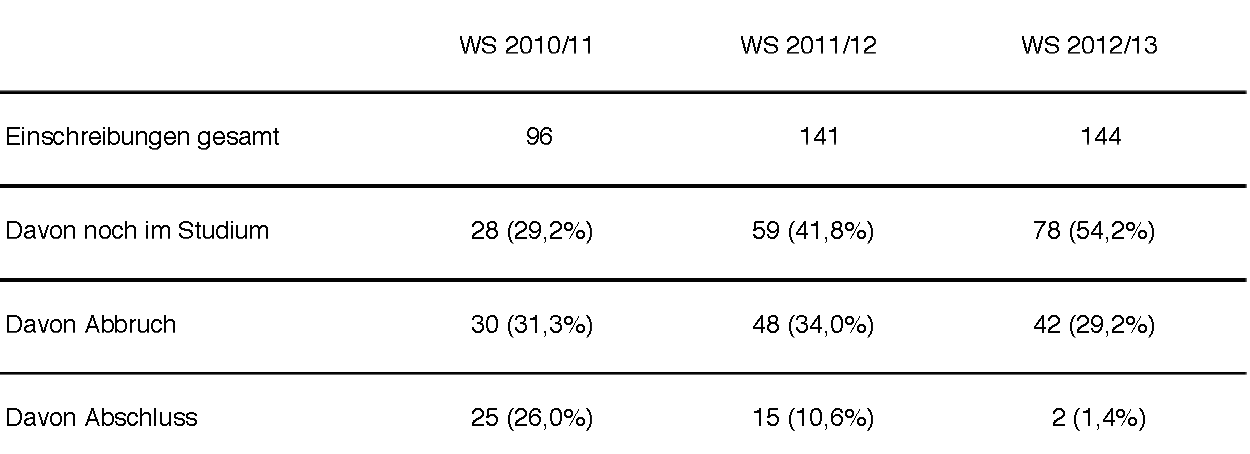
\includegraphics[width=\columnwidth]{../anhaenge/tabellen/MI-BA-anzahl-studierende.pdf}
\caption{Tabelle: Daten des Bachelorstudiengangs Medieninformatik}
\end{figure}

\begin{longtable}[]{@{}lllll@{}}
\toprule
\begin{minipage}[b]{0.11\columnwidth}\raggedright\strut
Semester\strut
\end{minipage} & \begin{minipage}[b]{0.23\columnwidth}\raggedright\strut
Einschreibungen gesamt\strut
\end{minipage} & \begin{minipage}[b]{0.22\columnwidth}\raggedright\strut
Davon noch im Studium\strut
\end{minipage} & \begin{minipage}[b]{0.14\columnwidth}\raggedright\strut
Davon Abbruch\strut
\end{minipage} & \begin{minipage}[b]{0.16\columnwidth}\raggedright\strut
Davon Abschluss\strut
\end{minipage}\tabularnewline
\midrule
\endhead
\begin{minipage}[t]{0.11\columnwidth}\raggedright\strut
WS 2010/11\strut
\end{minipage} & \begin{minipage}[t]{0.23\columnwidth}\raggedright\strut
96\strut
\end{minipage} & \begin{minipage}[t]{0.22\columnwidth}\raggedright\strut
28 (29,2\%)\strut
\end{minipage} & \begin{minipage}[t]{0.14\columnwidth}\raggedright\strut
30 (31,3\%)\strut
\end{minipage} & \begin{minipage}[t]{0.16\columnwidth}\raggedright\strut
25 (26,0\%)\strut
\end{minipage}\tabularnewline
\begin{minipage}[t]{0.11\columnwidth}\raggedright\strut
WS 2011/12\strut
\end{minipage} & \begin{minipage}[t]{0.23\columnwidth}\raggedright\strut
141\strut
\end{minipage} & \begin{minipage}[t]{0.22\columnwidth}\raggedright\strut
59 (41,8\%)\strut
\end{minipage} & \begin{minipage}[t]{0.14\columnwidth}\raggedright\strut
48 (34,0\%)\strut
\end{minipage} & \begin{minipage}[t]{0.16\columnwidth}\raggedright\strut
15 (10,6\%)\strut
\end{minipage}\tabularnewline
\begin{minipage}[t]{0.11\columnwidth}\raggedright\strut
WS 2012/13\strut
\end{minipage} & \begin{minipage}[t]{0.23\columnwidth}\raggedright\strut
144\strut
\end{minipage} & \begin{minipage}[t]{0.22\columnwidth}\raggedright\strut
78 (54,2\%)\strut
\end{minipage} & \begin{minipage}[t]{0.14\columnwidth}\raggedright\strut
42 (29,2\%)\strut
\end{minipage} & \begin{minipage}[t]{0.16\columnwidth}\raggedright\strut
2 (1,4\%)\strut
\end{minipage}\tabularnewline
\bottomrule
\end{longtable}

Die in Tabelle 1 dargestellten Zahlen zeigen einen stetig wachsenden
Zulauf für den Bachelorstudiengang Medieninformatik, der ursprünglich
für 63 Studierende ausgelegt wurde. Erfreulicherweise ist, trotz der im
Rahmen der Fakultätsentwicklung und des Hochschulentwicklungsplans
2020\footnote{\href{https://www.verwaltung.th-koeln.de/imperia/md/content/verwaltung/broschueren_leitfaeden/hochschulentwicklungsplan2020.pdf}{Hochschulentwicklungsplan
  2020} (abgerufen am 13.02.2017)} steigenden Anfängerzahlen, eine
gleichbleibende Abbrecherquote um die 30\% zu erkennen. Die Zahlen
zeigen leider auch eine niedrige Quote an Absolventen in
Regelstudienzeit, die jedoch im Mittel aller Studiengänge der Fakultät
10 liegt. Nach den vorliegenden Prüfungsstatistiken (vgl.
Prüfungsstatistiken \footnote{\href{../anhaenge/pruefungsstatistiken.pdf}{Bachelorstudiengang
  Medieninformatik, Prüfungsstatistik 2016}}) ist mit einem
proportionalen Anstieg der Absolventen zu rechnen.

\begin{verbatim}
@Volker: kann die Tabellennummerierung automatisiert werden?
\end{verbatim}

Die im Rahmen der letzten Reakkreditierung eingebrachten Änderungen
können hinsichtlich der Quote der Studienabbrecher bereits als recht
erfolgreich bewertet werden. Vor allem die Auflösung der strikten, durch
Zulassungsvoraussetzungen in der Prüfungsordnung verankerte Trennung von
Grund- und Hauptstudium hat die Dauer des Fachstudiums definitiv
verkürzt. Auch die Einführung des Moduls „Einführung in die
Medieninformatik`` (EMI) erweist sich als sinnvoll und notwendig, um den
Studierenden früh die Perspektiven und fachlichen Aspekte der
Medieninformatik näher zu bringen.

Aus der INCHER-Studie von 2014\footnote{\href{../anhaenge/INCHER-Studie.pdf}{INCHER-Studie
  2014}} geht für alle Studiengänge in NRW hervor: Wer während des
Studiums ein Firmenpraktikum absolviert, schließt das Studium etwas
seltener in der Regelstudienzeit ab (54 Prozent vs.~60 Prozent). Ähnlich
ist eine Tendenz zwischen denjenigen, die ihr Studium hauptsächlich
durch Erwerbsarbeit finanzierten und den übrigen Absolventinnen und
Absolventen zu erkennen: Wenn das Studium durch eigene Erwerbsarbeit
finanziert wurde, wird es ebenfalls seltener in der Regelstudienzeit
abgeschlossen (50 Prozent vs.~57 Prozent).

Schlussfolgerungen über die Studienqualität sind auf Grundlage der
verfügbaren Daten nur bedingt möglich. Als Ausgangspunkt für die, im
Rahmen der Reakkreditierung anzustrebenden Änderungen, wurden daher
zusätzlich folgende Quellen mit einbezogen:

\begin{itemize}
\tightlist
\item
  Studentische Rückmeldungen aus den, im Rahmen des Medieninformatik
  Showcase stattfindenden Feedbackrunden
\item
  Persönliche Gespräche mit Studierenden, Alumni und
  Kooperationspartnern
\item
  Probleme und Fragen, die an die Medieninformatik Mentorin und die
  Studiengangsmanager gerichtet wurden
\item
  Befragung der beteiligten Professoren, wissenschaftlichen Mitarbeitern
  und Tutoren
\item
  Rückschlüsse aus Veranstaltungsevaluationen
\item
  Gespräche mit Unternehmensvertretern
\end{itemize}

Auf dieser Basis konnten, bezogen auf die bereits beschrieben
Erkenntnisse der INCHER-Studie, zwei Gründe für verlängerte Studiendauer
ermittelt werden:

\begin{itemize}
\tightlist
\item
  Viele Studierende finanzieren ihr Studium, vor allem in höheren
  Semestern und im Master-Studium, durch Erwerbsarbeit.
\item
  Das große Modul ``Entwicklungsprojekt interaktive Systeme'' (10
  Creditpoints) überfordert viele Studierende.
\item
  Das Praxisprojekt im sechsten Semester wird in der Regel in
  Kooperation mit Unternehmen absolviert.
\end{itemize}

Bei den Vorbereitungen zum Praxisprojekt, das in der Regel im selben
Themenfeld wie die Bachelorarbeit absolviert wird, durchlaufen die
Studierenden in der Regel einen dreistufigen Prozess:

\begin{enumerate}
\def\labelenumi{\arabic{enumi}.}
\tightlist
\item
  Identifikation eines geeigneten Themenfeldes für das Praxisprojext, in
  der Regel in Absprache mit einem oder mehreren Dozenten.
\item
  Bewerbung bei passenden Kooperationspartnern in der Wirtschaft.
\item
  Einarbeitung beim Unternehmen und Einigung auf das finale Thema zum
  Praxisprojekt mit dem Unternehmen und dem Dozenten.
\end{enumerate}

Dieser Prozess ist zeitaufwändig und wird von den meisten Studierenden
unterschätzt und daher häufig zu spät begonnen. Um diesem Problem
entgegen zu wirken wird in der Medieninformatik seit drei Jahren am Ende
des fünften Semesterseine Kontaktbörse durchgeführt. Auf dieser
Veranstaltung werden den künftigen Absolventen die Regularien, Abläufe
und Herausforderungen des Abschlusssemesters erläutert. Darüber hinaus
stellen ausgewählte Unternehmen und Organisationen potenzielle Themen
und Problemfelder für Praxisprojekt und Bachelorarbeit vor. Auch die
Professoren der Informatik haben hier die Möglichkeit ihre Themen und
Forschungsfelder als Ansatzpunkt für mögliche, forschungsnahe
Praxisprojekte und Abschlussarbeiten vorzustellen.

\subsection{Bewertung von Ergebnissen aus
Evaluationen}\label{bewertung-von-ergebnissen-aus-evaluationen}

Hier kann auf Erstsemesterbefragungen und regelmäßig semesterweise
durchgeführte Evaluationen der Lehrveranstaltungen verwiesen werden. Die
Auswertung der Evaluationen erfolgt zentral durch das Hochschulreferat 4
\emph{Qualitätsmanagement}. Darüber hinaus ist an der Fakultät 10 ein
integriertes Qualitätsmanagement nach DIN/ISO 9001 etabliert. In den
Ergebnissen\footnote{\href{../anhaenge/evaluationen-f10.pdf}{Studentische
  Evaluationen Medieninformatik}} zeigt sich grundsätzlich bei den
Bachelorstudierenden ein etwas geringeres Zufriedenheitsmaß als bei den
Masterstudierenden. Dies lässt sich mit Verweis auf die allgemein hohen
Abbruchquoten in grundständigen Informatikstudiengängen ggf. so
interpretieren, dass die Unzufriedenheit nicht allein durch die
Studienangebotsseite verursacht ist. Dennoch lassen sich deutliche
Verbesserungspotentiale identifizieren, etwa bzgl. der Einführung neuer
Lehr- und Lernformate, Koordination der Praktika, Bereitstellung von
studentischen Arbeitsräumen, Gastvorträgen, Exkursionen und Workshops.

Der 2013 zu verzeichnende Rückgang der Zufriedenheit bzgl. des
Lehrangebotes im Master lässt sich nach unseren Analysen und Gesprächen
mit Studierenden u.A. als Auswirkung des ersten, im Informatik-Master
durchgeführten Projekt-Semesters interpretieren. Die dort durchgeführten
„Guided Projects`` zeigen einen starken Praxisbezug und eine klare, mit
den Methoden des (oft agilen) Projektmanagements gestaltete
Ablaufstruktur. Diese auf den Arbeitsmarkt ausgerichtete
Herangehensweise wird auch von vielen Studierenden im Medieninformatik
Master gewünscht.

Die Unzufriedenheit bei der Bewertung der Studien- und
Prüfungsorganisation in der Fakultät lässt sich auf punktuelle Ausfälle
des ``Prüfungs- und Studierendenservice Online'' (PSSO) und teilweise
nicht optimal im Internet kommunizierte Prüfungsinformationen
zurückführen. Erfreulich ist die weiterhin große Gesamtzufriedenheit der
Studierenden im Medieninformatik Master.

\subsection{Bewertung der statistischen Daten bezüglich der
Auslastung, der Prüfungserfolge, der Abbrecherquoten und der
Studienanfänger- und
Bewerberzahlen.}\label{bewertung-der-statistischen-daten-bezuxfcglich-der-auslastung-der-pruxfcfungserfolge-der-abbrecherquoten-und-der-studienanfuxe4nger--und-bewerberzahlen.}

Die folgenden Ausführungen beruhen auf der Datenerhebung zum 22.09.2016
für den Zeitraum Wintersemester 2011 bis Wintersemester 2015\footnote{\href{../anhaenge/pruefungsstatistiken.pdf}{Bachelorstudiengang
  Medieninformatik, Prüfungsstatistik 2016}}\footnote{\href{../anhaenge/Fakultaetsstruktur-Studienangebot-Personal-Haushaltsmittel-Kennzahlen-2014.pdf}{Fakultät
  für Informatik und Ingenieurwissenschaften, Statistik 2013/14}} und
fokussieren die derzeit eingeschriebenen Studenten, erfolgreiche
Abschlüsse und Studienfachabbrecher.

Zur Bewertung der Auslastung kann wie folgt Stellung genommen werden:
Gemessen an den planmäßigen 63 Studierendenplätzen (WS13/14) werden seit
drei Studienjahren im Rahmen der strategischen Fakultätsplanung und des
Hochschulentwicklungsplans 2020 mehr als 200\% Überlast aufgenommen. Mit
den Abbrecherquoten im Bachelorstudiengang bewegt sich die
Medieninformatik im breiten Mittelfeld von Informatikstudiengängen im
Allgemeinen\footnote{\href{http://www.dzhw.eu/pdf/pub_fh/fh-201503.pdf}{Ulrich
  Heublein et al.: Studienbereichsspezifische Qualitätssicherung im
  Bachelorstudium - Befragung der Fakultäts- und Fachbereichsleitungen
  zum Thema Studienerfolg und Studienabbruch. Forum Hochschule, 3/2015}
  (abgerufen am 13.02.2017)}; sehr erfreulich ist für den
Masterstudiengang Medieninformatik die geringe Abbrecherquote. In
Verbindung mit der bedauerlich hohen, für ingenieur- und
naturwissenschaftliche Studiengänge, insbesondere im Bachelor-Bereich
jedoch leider inhärenten Abbrecherquote (durchschnittlich geschätzte
Schwundquote in der Informatik an Fachhochschulen ist 39\%\footnote{\href{http://www.dzhw.eu/pdf/pub_fh/fh-201503.pdf}{Ulrich
  Heublein et al.: Studienbereichsspezifische Qualitätssicherung im
  Bachelorstudium - Befragung der Fakultäts- und Fachbereichsleitungen
  zum Thema Studienerfolg und Studienabbruch. Forum Hochschule, 3/2015}
  (abgerufen am 13.02.2017)}), zeigt sich hier ein deutliches noch zu
hebendes Optimierungspotential. Erfreulich ist hier die mit 27\% recht
hohe Frauenquote im Bachelorstudiengang Medieninformatik. Die
durchschnittliche Frauenquote in der Lehreinheit Informatik liegt bei
22\%. In der Fakultät 10 liegt sie bei 20\%.

Die Prüfungserfolge sind bzgl. des Bachelor- und Masterstudiengangs zu
differenzieren.

Im Bachelorstudiengang Medieninformatik zeigt sich bei den
Prüfungserfolgen des „neuen`` im Vergleich zum „alten`` Studiengang
(BPO2 vs.~BPO3, s. Anhang Pruefungsstatistiken \footnote{\href{../anhaenge/pruefungsstatistiken.pdf}{Bachelorstudiengang
  Medieninformatik, Prüfungsstatistik 2016}}) ein früherer
Prüfungserfolg. Auch in höheren Semestern werden die Prüfungen früher
absolviert und mit weniger Fehlversuchen bestanden. In erster Näherung
findet man in den ersten beiden Semestern eine Gleichverteilung der
Noten innerhalb des Notenspektrums, die sich in den höheren Semestern zu
einer deutlichen Verbesserung hin verschiebt. Hier mögen zwei Faktoren
von Bedeutung sein: Zum einen der deutlich höhere Anteil an
medien(informatik)spezifischen Modulen und zum anderen kann gemutmaßt
werden, dass sich hier die Abbrecherzahlen positiv auswirken. Die
Abschluss- und die Endnoten setzen diesen Trend der Verbesserung des
Notendurchschnitts fort.

Im Masterstudium wirkt sich die im Rahmen der Reakkreditierung
weggefallene Zulassungsvoraussetzung eines Mindest-Notenschnittes nicht
wesentlich auf die Verteilung der Prüfungsergebnisse aus. Auch hier ist
weiterhin das gesamte Notenspektrum abgedeckt, ebenso wie bei den
Ergebnissen der Master Thesen. \textsubscript{\textasciitilde{}} mw:
haben wir für den MAster eine Prüfungsstatistik?
\textsubscript{\textasciitilde{}}

\subsection{Rückschlüsse aus informellen Gesprächen und
Kommentaren}\label{ruxfcckschluxfcsse-aus-informellen-gespruxe4chen-und-kommentaren}

\begin{quote}
\ldots{} anstrengend und fordernd, aber macht viel Spaß \ldots{}
\end{quote}

Aus verschiedenen Einzel- und Gruppengesprächen im Team der
Studiengangsbetreiber, Gesprächen mit Studierenden und Alumni,
Kommentaren von Feedbackrunden sowie Online-Foren lassen sich eine Reihe
von Stärken und Schwächen ableiten.

Der Studienaufbau des Bachelorstudiengangs wird überwiegend als positiv
und gut durchdacht bewertet. Die Lehrveranstaltungen werden in Summe als
gut organisiert und vorbereitet, interessant, aber auch als sehr sehr
anspruchsvoll beschrieben. Der Umfang des Studiums wird zuweilen als
``vom Umfang überwältigend'' bezeichnet. Diese Einschätzung wird von
Alumni jedoch dahingehend ergänzt, dass nach dem Einstieg ins
Berufsleben die Wichtigkeit und Relevanz der einzelnen Module offenbar
wurde, sie sich mit dem Studium sehr gut im Beruf platzieren konnten und
in bestimmten Berufszweigen sehr flexibel einsetzbar sind. Das
Verhältnis der allgemeinen Informatik Anteile und der
medieninformatik-spezifischen Module wird gut bewertet.

Durchweg sehr positiv wird die gute und intensive Betreuung durch das
Lehrpersonal beschrieben: ``Die Dozenten sind super hilfreich
\ldots{}''. Dies gilt auch für die vielen praktischen Projekte und
Gruppenarbeiten. Auch die Offenheit für eigene Ideen und die
Gruppengröße bei den Praxisanteilen wird sehr positiv bewertet. Das
Mentoring-Programm wird ebenfalls als sehr hilfreich wahrgenommen.

Auch sehr positiv wird die gute und moderne Ausstattung der
Medieninformatik und der Bibliothek, als auch der recht ausgewogene
quantitative Verhältnis von Frauen und Männern bewertet.

Als problematisch wird, bezogen auf den Bachelorstudiengang, vor allem
die starke Fragmentierung der Module sowie der zugehörigen Praxisanteile
gesehen, sodass die Situation, vor allem im dritten Fachsemester, als
``zu voll'' oder mit ``zu viele Baustellen'' beschrieben wird. Dieses
Problem wurde auch im Rahmen der Analysen zum Profil2 Antrag der
Hochschule identifiziert \footnote{\href{https://www.th-koeln.de/mam/downloads/deutsch/hochschule/profil/lehre/profil2_antrag_ministerium.pdf}{Profil2
  Antrag der TH Köln} (abgerufen am 15.02.2017)}. Derzeit wird dieser
Problematik bereits mit der sequentiellen Anordnung einiger Module
begegnet. Dabei werden zwei parallel laufende Module nacheinander, dafür
aber mit halber Laufzeit und doppelter SWS Anzahl angeboten, so dass
sich die Studierenden auf weniger Module zur gleichen Zeit konzentrieren
können. Diese Herangehensweise wurde ebenfalls im Rahmen von Profil2 als
Maßnahme vorgeschlagen\footnote{\href{https://www.th-koeln.de/mam/downloads/deutsch/hochschule/profil/lehre/profil2_antrag_ministerium.pdf}{Profil2
  Antrag der TH Köln} (abgerufen am 15.02.2017)}. Viele Studierende
wünschen sich die Möglichkeit der Fachvertiefung. Das Problem wird
häufig mit ``man kratzt alles nur an und dann kommt schon das nächste
Thema'' beschrieben. Gerade bei den Implementierungs-affinen
Studierenden, aber auch bei den Lehrenden wird häufig der Wunsch nach
mehr Unterstützung im Bereich Programmierung genannt. Dies gilt vor
allem für komplexere und größere Projekte. Derzeit fehlt im
Bachelorprogramm ein Modul, dass die Studierenden auf die rechtlichen
Fragestellung in der (Medien-)Informatik vorbereitet. Dieses Defizit
wurde in verschiedenen Feedbackrunden adressiert.

Bezogen auf den Master wird immer wieder die fehlende oder unzureichende
Praxisorientierung als Problem genannt. Auch hier fehlt den Studierenden
die Möglichkeit zur Fachvertiefung entsprechend der persönlichen
Neigung.

\subsection{Ableitungen aus den Bewertungen der zur Verfügung
stehenden Daten und
Evaluationen}\label{ableitungen-aus-den-bewertungen-der-zur-verfuxfcgung-stehenden-daten-und-evaluationen}

Aus den Bewertungen der Daten, Evaluationen und Feedbacks lassen sich
folgende Problem und Schwächen ableiten.

\paragraph{Medieninformatik Bachelor}\label{medieninformatik-bachelor}

Als Indikator für eine gute Studierbarkeit, kann die Anzahl der
abgelegten Prüfungen im vorgesehenen Fachsemester des Moduls angesehen
werden. Ziel ist es, dass die Studierenden Prüfungen möglichst im selben
Semester ablegen, in dem das Modul im Studienverlaufsplan verortet ist.
Gelingt dies nicht, so kann ein Studienabschluss innerhalb der
Regelstudienzeit fast nicht mehr realisiert werden. Ab dem dritten
Studiensemester werden Prüfungen zunehmend verspätet abgelegt (vgl.
Pruefungsstatistiken\footnote{\href{../anhaenge/pruefungsstatistiken.pdf}{Bachelorstudiengang
  Medieninformatik, Prüfungsstatistik 2016}}). Feedbacks, Befragungen
und Curriculumsanalyse\footnote{fehlt} zeigen, dass in diesem Semester
die Anzahl der unterschiedlichen Module am höchsten ist und viele Module
Praxisanteile in Projektform haben, sodass sich die Studierenden in
verschiedene Fachdisziplinen, Modulregularien und Projektkontexte
eindenken und vielen Teamkonstellationen organisieren müssen.
Darüberhinaus sind im dritten Semester bei vielen Modulen
Prüfungsvorleistungen (Teilnahmeschein) notwendig.

Ein weiteres Problem bildet offenbar das große Projekt im fünften
Semester (Entwicklungsprojekt interaktive Systeme). Nachdem die
Studierenden in den vorangegangen Semestern nur mit Projektgrößen von
maximal 2,5 Creditpoints konfrontiert wurden, stehen sie im fünften
Semester einem Projekt der vierfachen Größe gegenüber. Dies scheint
viele zu überfordern, so dass sie entweder erst dann das Projekt
beginnen, wenn sie keine parallelen Veranstaltungen haben, oder das
Projekt vorzeitig abbrechen.

Die Probleme beim Übergang ins Abschlusssemester wurden bereits
beschrieben. Vor allem in Feedbacks und persönlichen Gesprächen wird ein
weiteres Defizit häufig genannt: Die fehlende Möglichkeit sich in einem
thematischen Bereich zu vertiefen.

Somit lassen sich die folgenden Defizite im aktuellen Medieninformatik
Bachelor Studiengang zusammenfassen:

\begin{itemize}
\tightlist
\item
  Überladenes drittes Fachsemester
\item
  Zu viele Projektkontexte
\item
  Zu großer Sprung der Projektgrößen
\item
  Zu viele verschiedene Module mit unterschiedlichen Regularien
\item
  Zeitproblem beim Einstieg ins Praxisprojekt
\item
  Fehlende Möglichkeit zur strukturierten Vertiefung
\item
  Übergang in den Spezialisierungsteil (vom vierten ins fünfte Semester)
  übergang ins Abschlussprojekt
\item
  zu starke Fragmentierung, zu wenige Zusammenhänge
\item
  zu viele „Baustellen``
\item
  keine Spezialisierung, zu allgemein
\item
  zu wenige Übergänge in den Master
\item
  kein Medienrecht
\item
  zu wenig Kenntnisse über verschiedene Programmierkonzepte
\item
  missverständliches Abschlusssemester
\end{itemize}

\paragraph{Medieninformatik Master}\label{medieninformatik-master}

Beim Medieninformatik Master leiten sich die erkannten Defizite im
Wesentlichen aus Feedbacks und persönlichen Gesprächen mit Studierenden,
Bachelor Absolventen und Dozenten ab. Die fehlende Möglichkeit zur
fachlichen Vertiefung und der geringe Anteil an praxisnaher Projekte
werden als wesentliche Defizite wahrgenommen und führen schlussendlich
auch dazu, dass viele potenzielle Studieninteressierte an andere
Studiengänge, zumeist außerhalb der TH Köln, mit stärkerer Profilierung
und Praxisbezug verloren gehen.

Der Medieninformatik Master sieht derzeit zwar verschiedene Wahlmodule
vor, diese sind aber stark fragmentiert und reglementiert, so dass hier
häufig keine echte Wahl durch die Studierenden getroffen werden kann.
Hinzu kommt, dass sich die Informatik Masterstudiengänge der Fakultät 10
sehr stark auseinander entwickelt haben, sodass Synergien, auch bei den
angebotenen Wahlpflichtfächern und Projekten nur schwer genutzt werden
können.

Somit lassen sich die folgenden Defizite im aktuellen Medieninformatik
Master Studiengang zusammenfassen:

\begin{itemize}
\tightlist
\item
  zu wenig Übergänge von Bachelorabsolventen des Campus Gummersbach
\item
  Fehlende Profilschärfung und sichbarer Praxisbezug
\item
  Geringer Anteil an praxisnahen Projekten
\item
  Geringe internationale Ausrichtung
\item
  Fehlende Möglichkeiten zur fachlichen Vertiefung
\item
  zu wenig Wahlmöglichkeiten
\end{itemize}

\chapter{Soll-Zustand/ geplante
Veränderungen}\label{soll-zustand-geplante-veruxe4nderungen}

Seit der Reakkreditierung der Medieninformatik Studiengänge vor sieben
Jahren haben sich sowohl die Berufsbilder der Absolventinnen und
Absolventen als auch der Diskurs über Curricula der Medieninformatik
weiterentwickelt. Wir sehen vor allem drei Felder, in denen die
Perspektive der Medieninformatik erhebliche Relevanz erlangt hat: - die
Modelle und Methoden der Mensch-Computer-Interaktion (MCI) haben sich
nicht zuletzt in der entsprechenden Fachgruppe der Gesellschaft für
Informatik (GI) als ein konstituierendes Element des Gebiets
``Medieninformatik'' herauskristallisiert. - die Entwicklung von
Anwendungen im und für das Web hat sich als ein zunehmend eigenständiges
Feld der Systementwicklung etabliert. Während die Wirtschaftsinformatik
und die allgemeine Informatik das Web als Plattform für
Geschäftsprozesse bzw. als technische Plattform in den Vordergrund
stellen, steht in der Medieninformatik das Web selbst als
gesellschaftliches und ökonomisches Phänomen im Vordergrund, das durch
die Vernetzung von Personen, Diensten, Daten und Dingen (``things'')
neue technische, soziale und ökonomische Qualitäten hervorruft. -
digitale Medien wie audiovisuelle Medien, Visualisierungen oder
virtuelle oder angereicherte Welten (``virtual and augmented
realities'') haben als eines der konstituierenden Felder der
Medieninformatik in den letzten Jahren stark an Bedeutung gewonnen. In
diesen drei Feldern beobachten wir auch, dass ein signifikanter Anteil
unserer Absolventinnen und Absolventen ihre berufliche Zukunft sucht.

Darüber hinaus hat das Institut für Informatik beschlossen, als
Zukunftsfeld den Bereich ``Social Computing'' zu gestalten. Hierunter
werden Methoden, Techniken und Modelle für den Einsatz von in der Regel
Web basierten IT Systemen im gesellschaftlicen Kontext subsummiert, also
etwa Lernsysteme, Assistenzsysteme oder auch Systeme für die
gesellschaftliche und politische Teilhabe. Dieses Feld wird zunächst als
Teil der Studiengänge der Medieninformatik aufgebaut.

\section{Weiterentwicklung des Lehrportfolios des Institut für
Informatik}\label{weiterentwicklung-des-lehrportfolios-des-institut-fuxfcr-informatik}

Im Antrag für die ``Anstehende Wiederzuweisung von fünf Professuren im
Institut für Informatik''\footnote{\href{../anhaenge/AntragWiederzuweisung_Motivation_2013.pdf}{AntragWiederzuweisung\_Motivation\_2013.pdf}}
wird der Lehr- und Forschungsbereich ``Soziotechnische Systeme'' wie
folgt argumentiert:

\begin{quote}
Die Informatik als wissenschaftliche Disziplin allgemein und auch das
Institut für Informatik im Besonderen muss sich der Tatsache stellen,
dass der technische und wissenschaftliche Fortschritt auf diesem
Fachgebiet nach wie vor rasant ist. Dem versucht das Institut nicht nur
durch stetige inhaltliche Weiterentwicklung seiner Studiengänge und
Module gerecht zu werden, sondern hier werden auch neue, auf
Nachhaltigkeit ausgerichtete Entwicklungen wahrgenommen und bei
ausreichender Relevanz in die Überlegungen zur Weiterentwicklung des
Angebots einbezogen. Eine solche -- aus Sicht des Instituts für
Informatik -- besonders interessante, spannende, wichtige und
zukunftsträchtige Entwicklung zeigt sich aktuell im Themenfeld
Soziotechnischer Systeme. Folgende Bereiche sind hier exemplarisch zu
nennen: - Assistenzsysteme für Tätigkeiten: Sportliches Training,
Navigation, Robotik (Staubsaugen, Lebensrettung, schwierige Umgebungen),
Autofahren, Büro, Produktionsumgebungen - Assistenzsysteme für
Bevölkerungsgruppen: alte Menschen, behinderte Menschen, Kinder,
Menschen im Alltag - Kommunikationshilfen: Suchmaschinen, soziale
Medien, Sprach-Ein- und Ausgabe, Blindenschrift-Displays und andere
spezielle Formen der MCI

In all diesen Bereichen zeichnet sich bereits heute eine große, künftig
noch stark zunehmende Bedeutung von IT-Systemen ab, zu deren Funktionen
nicht nur technisches Wissen, sondern auch Fach- und Methodenwissen aus
unterschiedlichen Spezialgebieten innerhalb der Informatik benötigt
wird. Um diesen neuen Entwicklungen gerecht zu werden, soll zunächst ein
geringer Anteil der Kapazität für dieses neue Themenfeld zur Verfügung
gestellt werden. Entsprechende Lehrveranstaltungen können und sollen
dann zunächst in Form von Wahlpflichtfächern angeboten werden. Die
entsprechenden Voraussetzung im Modulkatalog werden, sofern
erforderlich, kurzfristig geschaffen. Pflichtfächer werden dadurch nicht
beeinträchtigt.

Das Themenfeld „IT für Menschen`` wird auf absehbare Zeit als attraktiv
angesehen, sowohl für Forscher als auch für Unternehmen und nicht
zuletzt vor allem auch für Studieninteressierte. Wegen der nicht nur
technischen Ausrichtung ist aufgrund bisheriger Erfahrungen auch ein
signifikanter Anteil weiblicher Studierender zu erwarten. Das Themenfeld
bietet darüber hinaus viele Anknüpfungsmöglichkeiten an bereits
vorhandene Kompetenzen: Datenbanken, Medieninformatik, Softwaretechnik,
Ergonomie, MCI, Kommunikationstechnik, technische Spezialthemen, mobile
Systeme und Anwendungen u. v. m.

Die starke Durchdringung der Gesellschaft mit leistungsfähigen,
zunehmend mobilen, mit umfangreicher Sensorik ausgestatteten Endgeräten,
eröffnet auch hier teilweise völlig neue Fragestellungen und
Möglichkeiten. In Kombinationen mit den bestehenden alten und anderen
neuen Schwerpunkten eröffnet der Studienbereich „IT für Menschen`` auch
ein neues Forschungsfeld. Mittelfristiges Ziel ist es, hier ein neues
Studienangebot zu realisieren, dass auch aus den vom Präsidium für
solche Zwecke in Aussicht gestellten neuen Professuren gespeist wird und
nicht zu Lasten vorhandener Ressourcen -- weder in der Lehreinheit
Informatik noch in der Lehreinheit Ingenieurwissenschaften -- geht. Das
benötigte Know-how ist zum großen Teil bereits vorhanden und soll durch
Wahlpflichtangebote in diesem Bereich ergänzt werden.
\end{quote}

Das Lehr- und Forschungsbereich ``Soziotechnische Systeme'' findet sich
in den zu akkreditierenden Curricula unter dem Begriff ``Social
Computing''. Dieser Themenkomplex soll im Bachelor Studienprogramm als
Vertiefungsmodul und im Master als Schwerpunkt verankert werden.

\section{Geplante Veränderungen des Bachelor-Studiengangs gegenüber
dem aktuellen
Akkreditierungszeitraum}\label{geplante-veruxe4nderungen-des-bachelor-studiengangs-gegenuxfcber-dem-aktuellen-akkreditierungszeitraum}

Die im Folgenden dargestellten geplanten Veränderungen des
Bachelorstudienprogramms dienen zur Beseitigung erkannter Schwächen
(vgl. Defizite Medieninformatik Bachelor).

\subsection{Verbesserungen des
Studienaufbaus}\label{verbesserungen-des-studienaufbaus}

\begin{figure}[htbp]
\centering
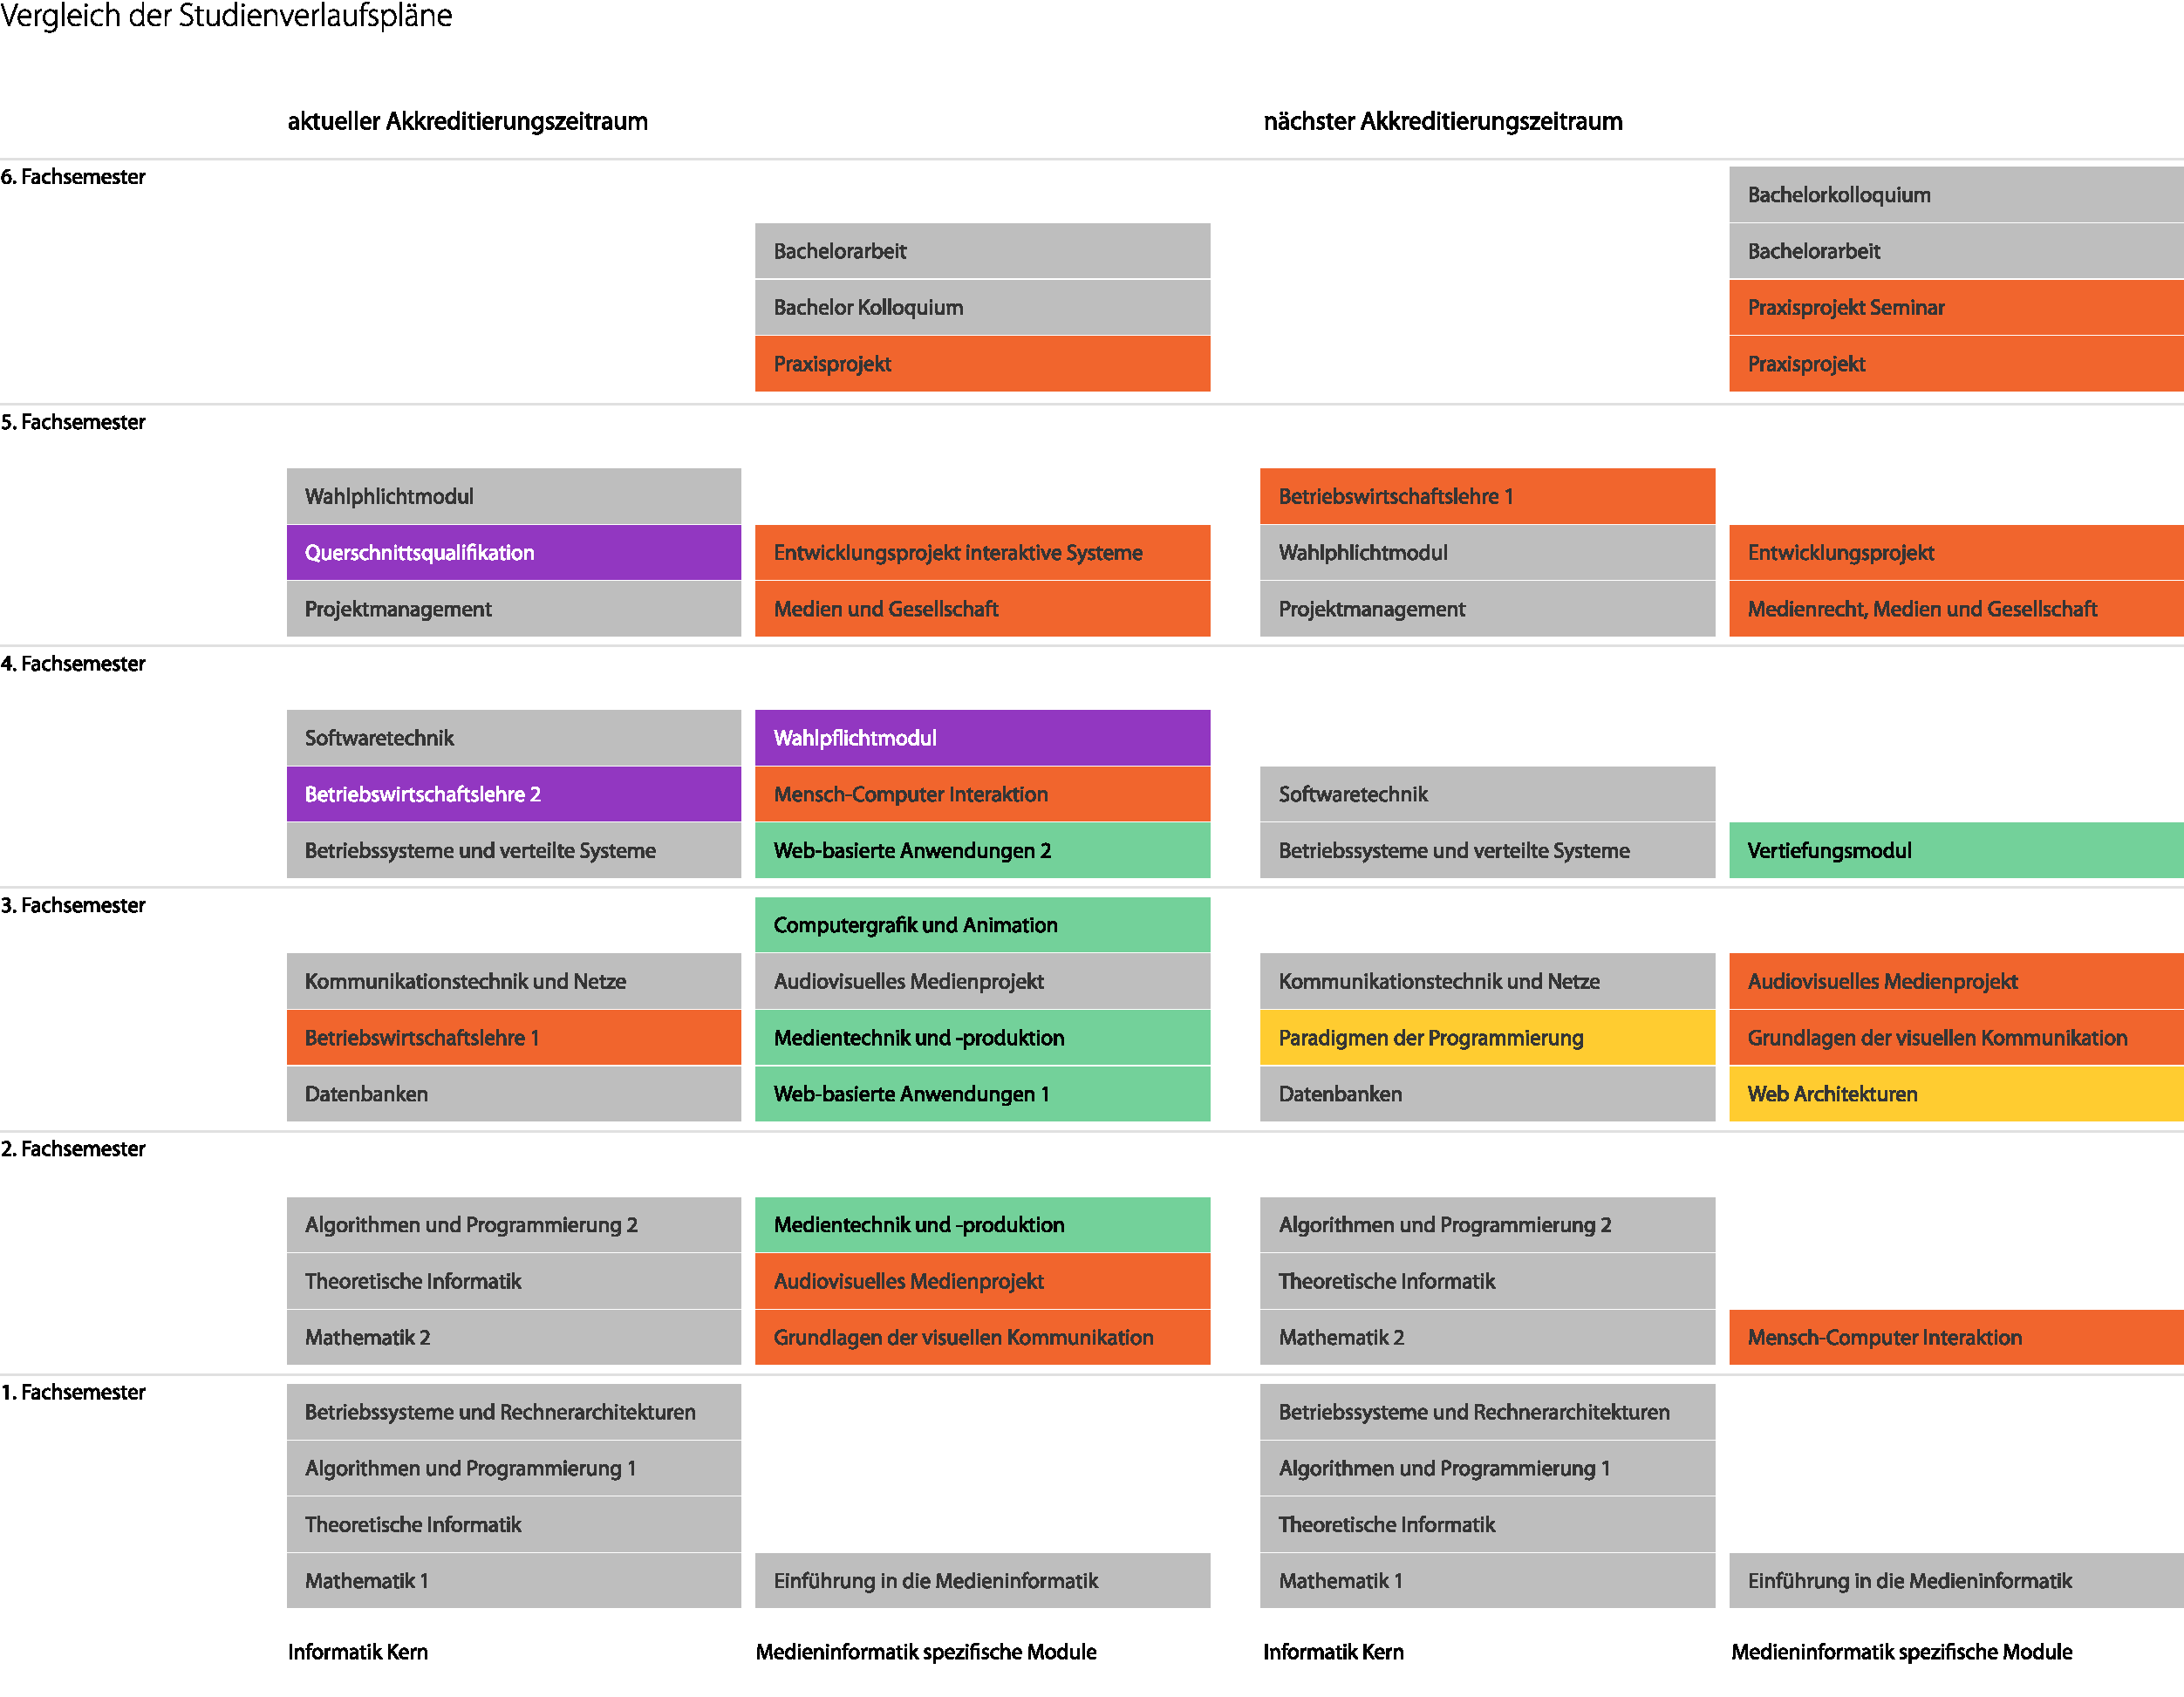
\includegraphics[width=\columnwidth]{../anhaenge/bilder/ba-veraenderungen-studienverlaufsplan.pdf}
\caption{Abbildung: Geplante Veränderungen des Bachelorstudiengangs
Medieninformatik. Links das aktuelle und rechts das zu akkreditierende
Curriculum. Die lila hinterlegten Module werden gestrichen, die grün
hinterlegten in Vertiefungsmodulen zusammengefasst, die orange
hinterlegten Module wurden neu angeordnet und die gelben Module wurden
neu integriert.}
\end{figure}

Mit einer Verbesserung des Studienaufbaus sollen folgende bekannte
Defizite ausgeglichen werden:

\begin{itemize}
\tightlist
\item
  Überladenes drittes Fachsemester
\item
  zu viele Projektkontexte
\item
  zu starke Fragmentierung von Modulen und der projektorientierten
  Praxisanteile
\item
  zu viele „Baustellen``
\end{itemize}

Die starke Projektorientierung wird und wurde insgesamt als positiv
bewertet. Jedoch ist die Verteilung der Module mit Projektanteil derzeit
nicht optimal. So sind z.B. im dritten Fachsemester momentan 7 Module
angesiedelt, von denen vier projektorientiert durchgeführt werden.
Hingegen wird im vierten Semester kein projektorientiertes Modul
angeboten. Um hier die Aufwände gleichmäßiger zu verteilen, wurde die
Reihenfolge der Module verändert und Module wurden zusammengelegt.

Beim Studienaufbau wurde versucht die Modulreihenfolge auf einen groben
Workflow der Softwareentwicklung auszurichten. Die prägnanteste
Auswirkung dieser Maßnahme ist die Verschiebung des Moduls
``Mensch-Computer Interaktion'' vom vierten ins zweite Semester, um die
Studierenden hier frühzeitig mit konzeptionellen Problemen und
Fragestellungen wie Tätigkeitsmodellierung oder die Spezifikation von
Anforderungen zu konfrontieren und ihnen hierzu entsprechende
Grundkenntnisse und Fertigkeiten zu vermitteln, die in den späteren
Projekten angewendet und eingeübt werden können.

Im vierten Semester wurde ein Vertiefungsmodul mit 20 Creditpoints
installiert auf das später noch weiter eingegangen wird. Bezogen auf den
Studienaufbau wird hierdurch die Fragmentierung und die vielen
Projektkontexte, die schlechtestenfalls mit vielen kleinen Modulen
einhergeht, deutlich reduziert.

\subsection{Verbesserter Aufbau der projektorientierten Module und
der
Projektgrößen}\label{verbesserter-aufbau-der-projektorientierten-module-und-der-projektgruxf6uxdfen}

\begin{figure}[htbp]
\centering
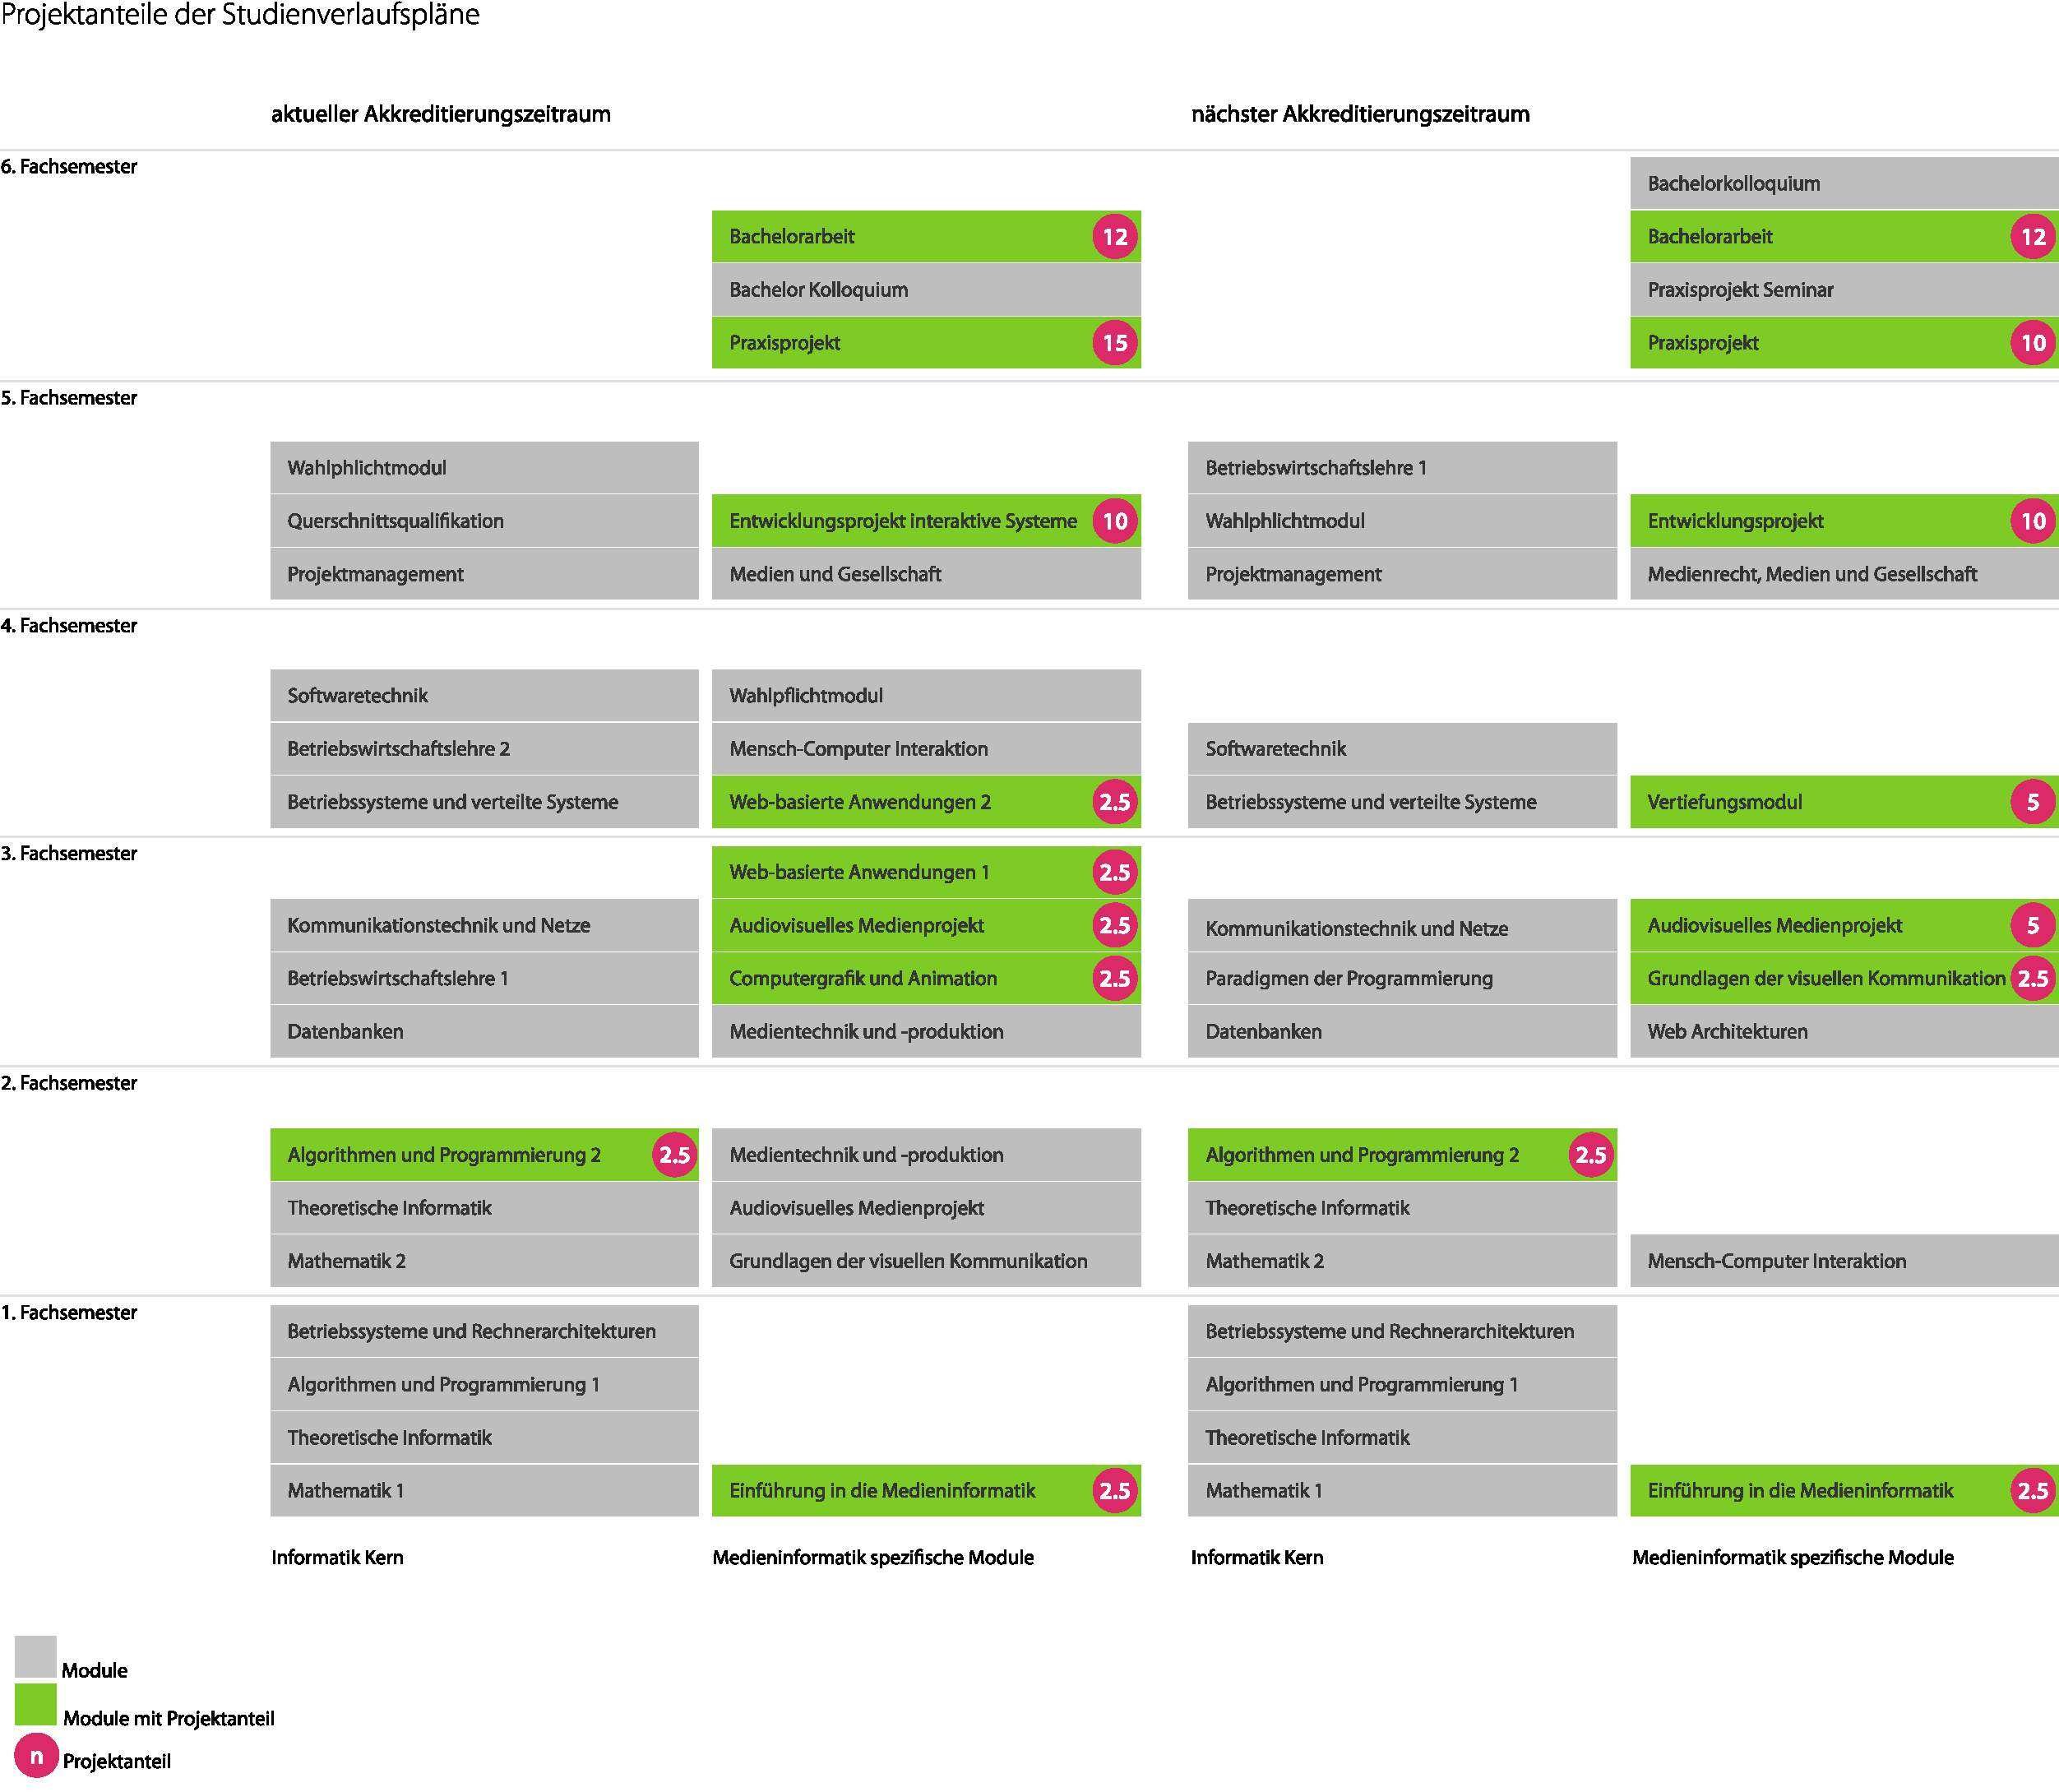
\includegraphics[width=\columnwidth]{../anhaenge/bilder/ba-projektanteile.pdf}
\caption{Abbildung: Veränderter Aufbau der Projektanteile des
Bachelorstudiengangs Medieninformatik. Links das aktuelle und rechts das
zu akkreditierende Curriculum.}
\end{figure}

Hiermit sollen folgende bekannte Defizite ausgeglichen werden:

\begin{itemize}
\tightlist
\item
  zu viele Projektkontexte
\item
  zu großer Sprung der Projektgrößen
\item
  zu viele „Baustellen``
\end{itemize}

Wie bereits beschrieben, wurden die projektorientierten Module
gleichmäßiger über den Studienverlauf verteilt und projektorientierte
Module teilweise zusammen gelegt. Um die Projektgrößen sinnvoll
aufzubauen, werden jetzt in den ersten drei Semestern Projekte mit einem
Gewicht von max. 2,5 Creditpoints absolviert. Im vierten Semester folgt
dann, als Teil des Vertiefungsmoduls, ein Projekt mit einem Gewicht von
etwa 5 Creditpoints. Im fünften Semester folgt dann das
Entwicklungsprojekt mit einem Gewicht von 10 Creditpoints. Im sechsten
Semester liegt dann das Praxisprojekt mit ebenfalls 10 Creditpoints und
die Bachelorarbeit mit 12 Creditpoints. Für diejenigen, die dann in
Masterstudiengang wechseln wollen, bleibt die Projektgröße dann bei 12
Creditpoints.

\subsection{Strukturierte Möglichkeit zur individuellen
Fachvertiefung}\label{strukturierte-muxf6glichkeit-zur-individuellen-fachvertiefung}

\begin{figure}[htbp]
\centering
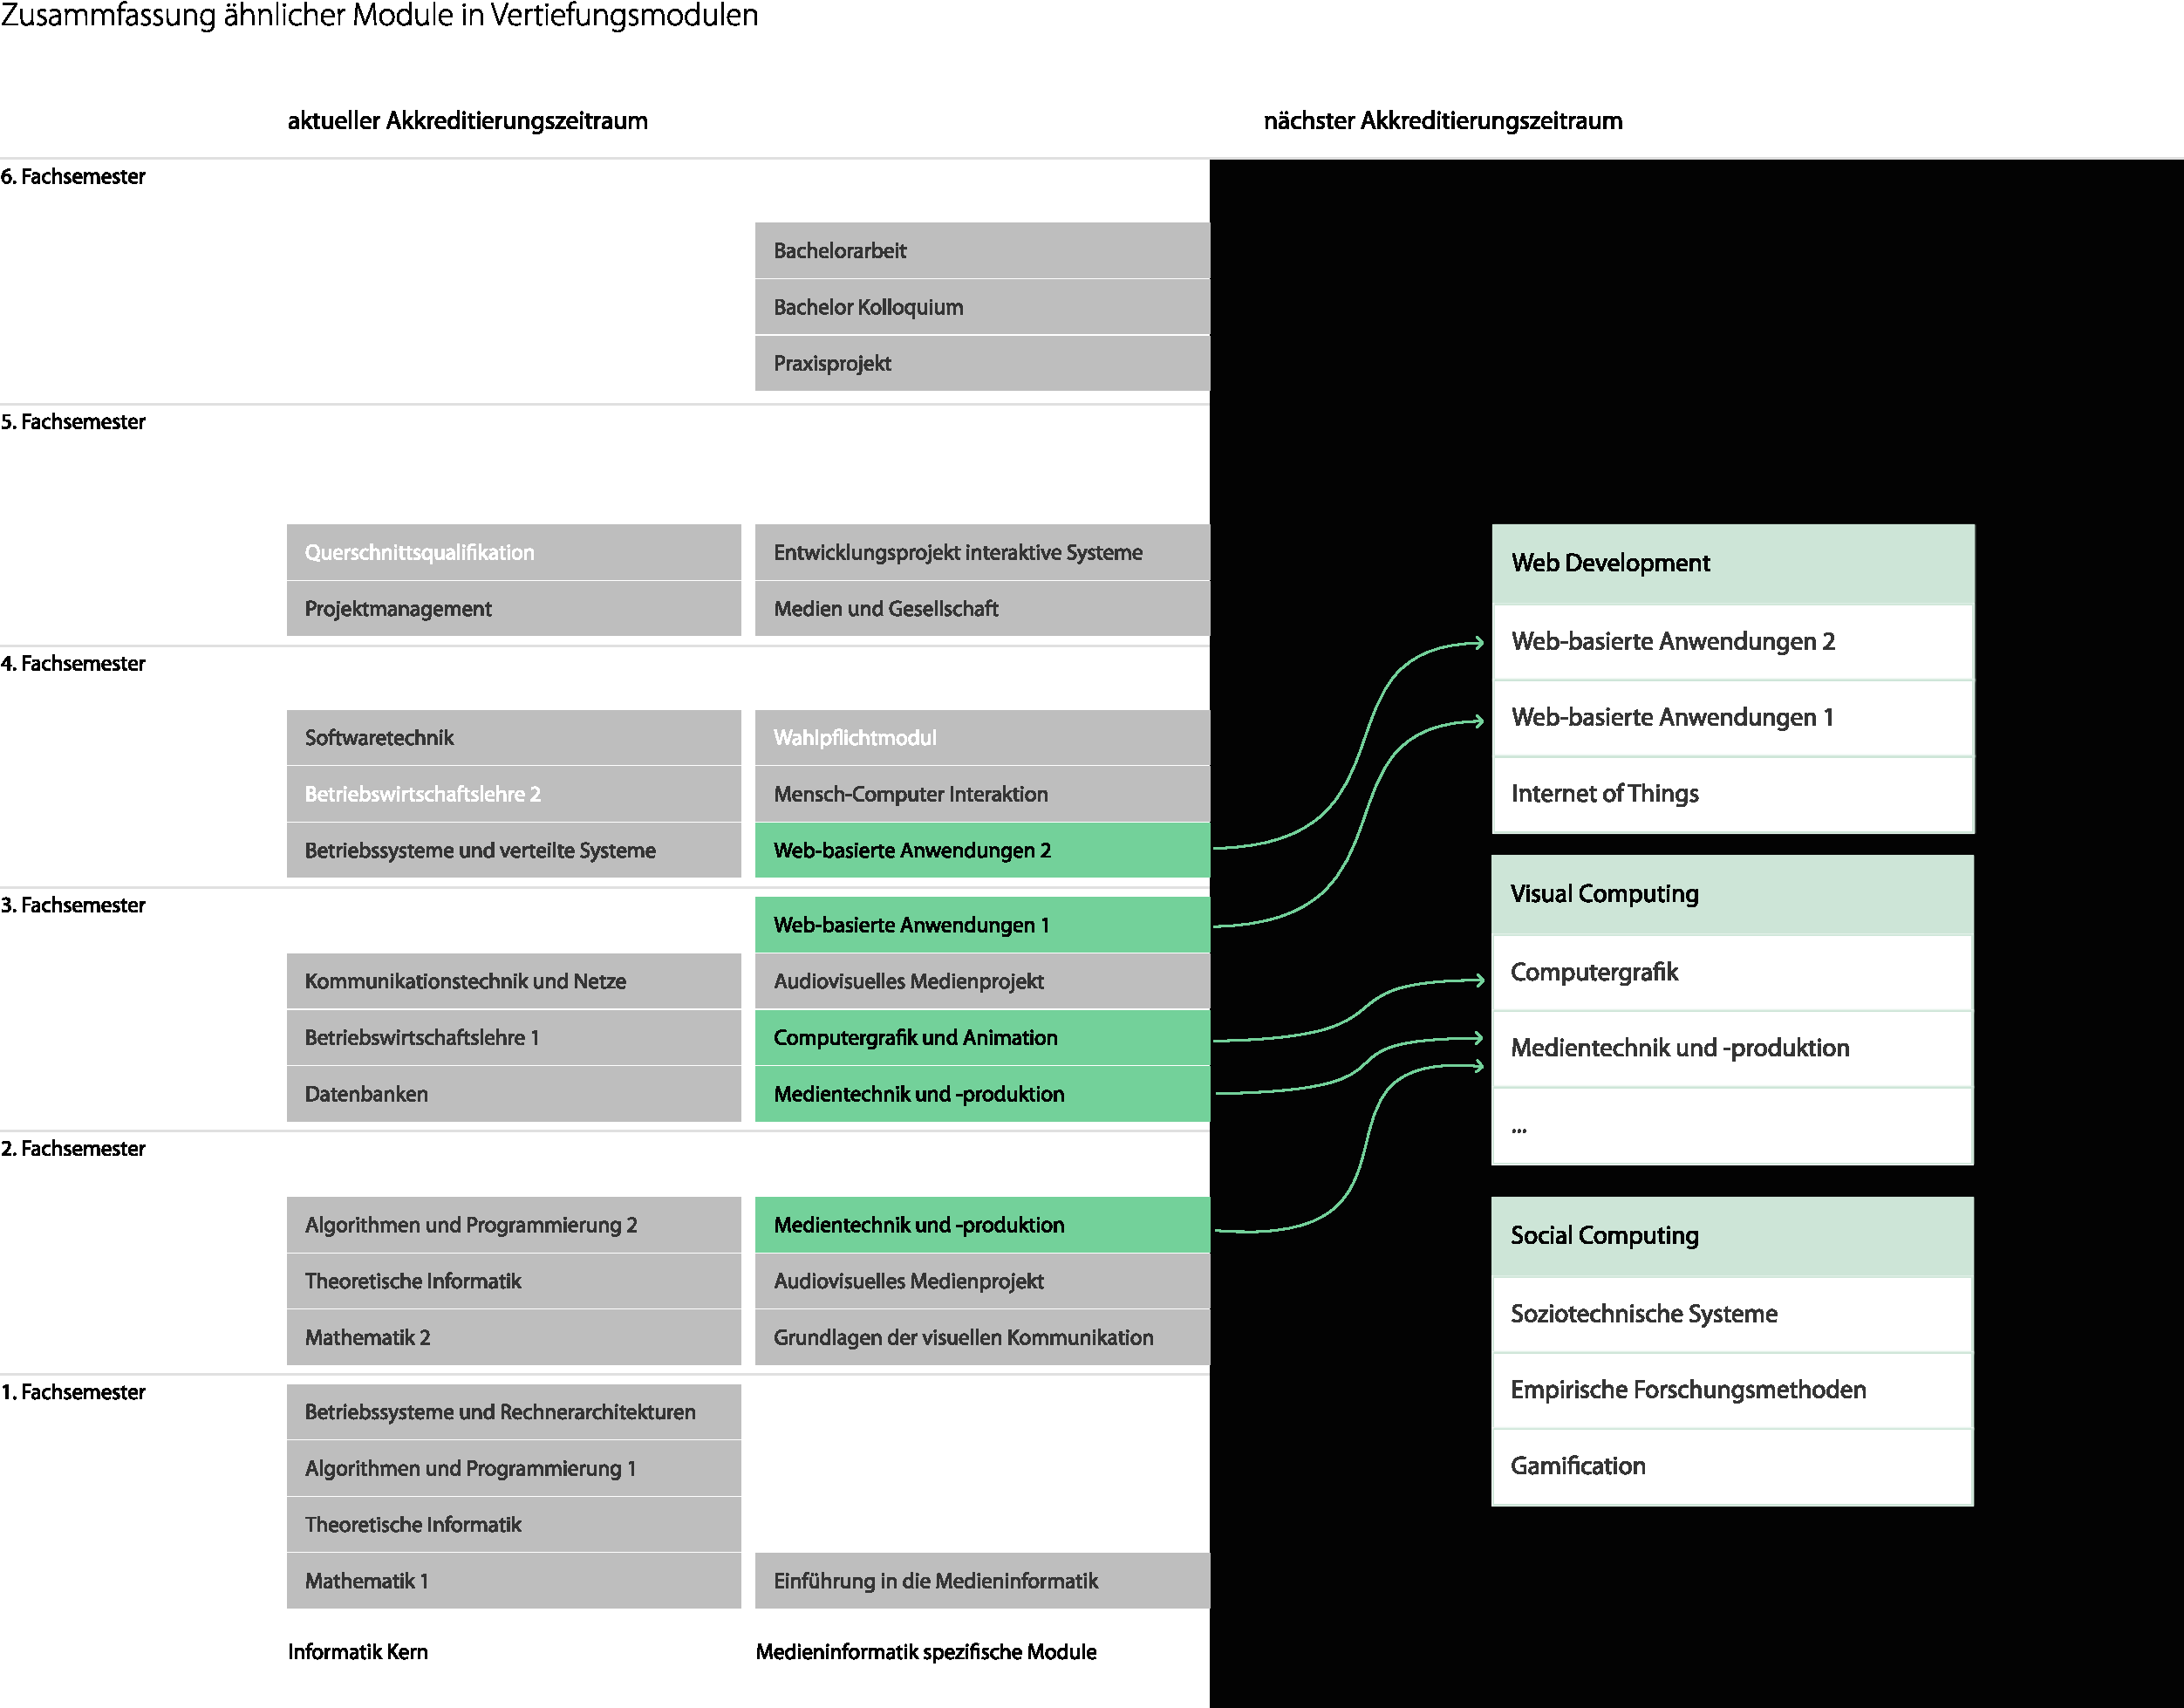
\includegraphics[width=\columnwidth]{../anhaenge/bilder/ba-vertiefungen.pdf}
\caption{Abbildung: Zusammenfassung von Modulen aus einem Themenfeld zu
Vertiefungsmodulen im Medieninformatik Bachelor.}
\end{figure}

Mit dieser Änderungen sollen folgende bekannte Defizite ausgeglichen
werden:

\begin{itemize}
\tightlist
\item
  keine Spezialisierung, zu allgemein
\item
  zu viele verschiedene Module mit unterschiedlichen Regularien
\item
  fehlende Möglichkeit zur strukturierten Vertiefung
\item
  zu viele Projektkontexte
\item
  zu großer Sprung der Projektgrößen
\item
  zu viele „Baustellen``
\item
  zu starke Fragmentierung von Modulen und der projektorientierten
  Praxisanteile
\item
  Übergang in den Spezialisierungsteil vom vierten ins fünfte
  Fachsemester
\item
  Übergang ins Abschlussprojekt
\item
  Zeitproblem beim Einstieg ins Praxisprojekt
\end{itemize}

Im vierten Semester wird ein Vertiefungsmodul mit einem Gewicht von 20
Creditpoints installiert. Hier stehen drei Vertiefungsrichtungen zur
Verfügung: Visual Computing, Social Computing und Web-Development. Im
Modul ist ein Projektanteil von etwa fünf Creditpoints vorgesehen. Mit
Hilfe des Vertiefungsmoduls werden eine Reihe von Schwächen
ausgeglichen. Die Studierenden haben hier die Möglichkeit tief in ein
Themenfeld einzudringen und darüber ggf. eine Spezialisierungsrichtung
einzuschlagen. Durch das Zusammenfassen mehrerer Module werden im
Vertiefungsmodul konsistente Regularien, sowie inhaltliche und
organisatorische Zusammenhänge geschaffen. Die Projektkontexte und die
inhaltlichen Perspektiven der Projekte werden reduziert. Der Übergang in
den Spezialisierungsabschnitt des Studiums im fünften Semester wird
idealerweise erleichtert, da durch die Wahl des Vertiefungsmoduls in
vielen Fällen schon eine Spezialisierungsrichtung vorgegeben ist.

Das Entwicklungsprojekt im fünften Semester wird inhaltlich geöffnet. Im
aktuellen Akkreditierungszeitraum war dieses Projekt fest an die
inhaltlichen Perspektiven ``Mensch-Computer Interaktion'' und
``Verteilte Anwendungen'' gebunden. Durch die inhaltliche Öffnungen
können die Studierenden jetzt ihre fachliche Vertiefung entsprechend
ihren Neigungen wählen. Damit geht die freie Wahl der betreuenden
Professoren einher. Idealerweise hat sich durch dieses Projekt und das
vorangegangene Vertiefungsmodul bereits eine inhaltliche und
organisatorische Zusammenarbeit gefestigt, die den Übergang ins
Abschlussprojekt deutlich erleichtert.

\subsection{Weitere Änderungen}\label{weitere-uxe4nderungen}

Darüber hinaus wurden weitere Änderungen durchgeführt, um die folgenden
Defizite zu verbessern:

\begin{itemize}
\tightlist
\item
  kein Medienrecht
\item
  missverständliches Abschlusssemester
\item
  zu wenig Kenntnisse über verschiedene Programmierkonzepte
\end{itemize}

Das Abschlusssemester wurde in seiner grundsätzlichen Struktur
beibehalten, jedoch wurde der Seminarteil das Moduls ``Praxisprojekt''
ausgelagert und als eigenes Modul installiert. Hiermit wird die
Studierbarkeit verbessert, da die zeitliche Kopplung des Praxis- und
Seminarteils reduziert wird. Darüber hinaus ist nun das Praxisprojekt
mit einem Gewicht von 10 Creditpoints ausgestattet und damit weniger
gewichtig, als die Bachelorarbeit, die ein Gewicht von 12 Creditpoints
hat.

Das Modul ``Paradigmen der Programmierung'', das bislang nur im
Informatik Bachelor als Pflichtmodul im Curriculum verankert war, wird
jetzt ein Pflichtmodul im dritten Fachsemester in der Medieninformatik
um die Studierenden bessere Kenntnisse im Bereich verschiedener
Programmierkonzepte und deren Anwendung zu vermitteln.

Da web-basierte Architekturen elementarer Bestandteil der
Medieninformatik und dediziert in den Studiengangszielen verankert sind,
wurde hierzu ein Pflichtmodul installiert, das Inhalte aus den Modulen
``Web-basierte Anwendungen 1 \& 2'' enthält, die alle Studierenden
kennen sollten, auch wenn sie sich später in einem anderen Bereich
vertiefen möchten.

Im fünften Semester wurde das Modul ``Medieninformatik und
Gesellschaft'' umgewidmet in ``Medienrecht, Medien und Gesellschaft'' um
hier einen dedizierten Platz für rechtliche Themen innerhalb der Domäne
im Curriculum zu verankern.

\section{Auswirkungen auf die
Lehrkapazität}\label{auswirkungen-auf-die-lehrkapazituxe4t}

Die Änderungen im Bachelorstudienprogramm sind weitgehend
kapazitätsneutral. Das von allen Informatikstudiengängen geteilte Modul
``Betriebswirtschaftslehre 2'' wurde durch des ebenfalls geteilte Modul
``Paradigmen der Programmierung'' ersetzt. Das Modul ``Mensch-Computer
Interaktion'' wurde zwar von fünf auf zehn Creditpoints vergrößert,
jedoch enthielt bislang das Modul ``Entwicklungsprojekt Interaktive
Systeme'' fünf Creditpoints Praxisanteil ``Mensch-Computer Interaktion''
die nun direkt dem Modul zugeschlagen werden.

Die Studierenden verteilen sich über die Vertiefungsmodule, in die auch
bisherige Wahlpflichtmodule integriert wurden. Somit reduziert sich hier
in Summe die Lehrbelastung. Durch die resultierende Reduktion ist es
möglich das Modul ``Web-Architekturen'' kapazitätsneutral anzubieten.
Das ``Entwicklungsprojekt'' im fünften Semester ist zukünftig nicht mehr
an nur zwei Lehrende gebunden, sondern kann von allen Lehrenden der
Informatik betreut werden. Dadurch verteilt sich die Lehrbelastung.

Lediglich das Vertiefungsmodul ``Social Computing'' ist nicht
kapazitätsneutral, hier wurde jedoch zusätzliche Kapazität aufgebaut.

\chapter{Geplante Veränderungen des Master-Studiengangs gegenüber dem
aktuellen
Akkreditierungszeitraum}\label{geplante-veruxe4nderungen-des-master-studiengangs-gegenuxfcber-dem-aktuellen-akkreditierungszeitraum}

Die im Folgenden dargestellten geplanten Veränderungen des
Masterstudienprogramms dienen zur Beseitigung erkannter Schwächen (vgl.
Defizite Medieninformatik Master). Grundsätzlich wurde die Basisgröße
der Module von fünf auf sechs Creditpoints erhöht. Module haben also
stets ein Gewicht von sechs Creditpoints oder einem Vielfachen davon.
Zum einen, um auch im Master die einzelnen Fachsemester weniger stark zu
fragmentieren, zum anderen, um mit dem Informatik Masterstudiengang, der
ebenfalls am Campus Gummersbach angeboten wird Module und Projekte
teilen zu können.

\section{Schärfung des Profils}\label{schuxe4rfung-des-profils}

Mit der Profilschärfung sollen folgende bekannte Defizite ausgeglichen
werden:

\begin{itemize}
\tightlist
\item
  zu wenig Übergänge von Bachelorabsolventen der eigenen Fakultät
\item
  Fehlende Profilschärfung und sichtbarer Praxisbezug
\item
  Fehlende Möglichkeiten zur fachlichen Vertiefung
\end{itemize}

Der Medieninformatik Masterstudiengang war bislang generalistisch
geprägt. Im Zuge der Reakkreditierung ist hier eine Veränderung
dahingehend geplant, dass Studierenden die Möglichkeit gegeben werden
soll, sich in bestimmten Bereichen zu spezialisieren. Dafür werden
Studienschwerpunkte geschaffen. Trotzdem soll weiterhin ein
generalistischer Studienverlauf möglich sein.

Aufbauend auf den thematischen Gebieten des Bachelorstudiengangs, die
sich dort unter anderem in den Vertiefungsmodulen manifestieren, und
ausgerichtet auf die Strategie des Instituts für Informatik, werden
folgende Schwerpunkte angeboten: ``Social Computing'', ``Visual
Computing'', ``Weaving the Web'' und ``Human-Computer Interaction''. Zur
Abbildung eines generalistischen Studienverlaufs wird der
Pseudo-Schwerpunkt ``Multiperspective Product Development'' angeboten,
der sich aus ausgewählten Modulen der anderen Schwerpunkte und des
Wahlpflichtkatalogs speist. Die Module der Schwerpunkte setzen sich zum
großen Teil aus bestehenden Modulen des Pflicht- und Wahlbereichs
zusammen. Für die Schwerpunkte ``Visual Computing'' und ``Social
Computing'' wurden einige neue Module erarbeitet, da hier, in Einklang
mit der inhaltlichen Strategie des Instituts, neue Themengebiete
erschlossen oder verbreitert werden sollen.

Die Schwerpunkte setzen sich aus den folgenden Modulen zusammen:

\subsection{Schwerpunkt Social
Computing}\label{schwerpunkt-social-computing}

\begin{longtable}[]{@{}lll@{}}
\toprule
\begin{minipage}[b]{0.33\columnwidth}\raggedright\strut
Modul\strut
\end{minipage} & \begin{minipage}[b]{0.33\columnwidth}\raggedright\strut
hervorgegangen aus\strut
\end{minipage} & \begin{minipage}[b]{0.33\columnwidth}\raggedright\strut
enthalten in folgenden Schwerpunkten\strut
\end{minipage}\tabularnewline
\midrule
\endhead
\begin{minipage}[t]{0.33\columnwidth}\raggedright\strut
Sicherheit, Privatsphäre und Vertrauen im Netz\strut
\end{minipage} & \begin{minipage}[t]{0.33\columnwidth}\raggedright\strut
IT Sicherheit\strut
\end{minipage} & \begin{minipage}[t]{0.33\columnwidth}\raggedright\strut
Multiperspective Product Development, Weaving the Web\strut
\end{minipage}\tabularnewline
\begin{minipage}[t]{0.33\columnwidth}\raggedright\strut
Soziotechnische Entwurfsmuster\strut
\end{minipage} & \begin{minipage}[t]{0.33\columnwidth}\raggedright\strut
-\strut
\end{minipage} & \begin{minipage}[t]{0.33\columnwidth}\raggedright\strut
-\strut
\end{minipage}\tabularnewline
\begin{minipage}[t]{0.33\columnwidth}\raggedright\strut
Netzwerk-und Graphentheorie\strut
\end{minipage} & \begin{minipage}[t]{0.33\columnwidth}\raggedright\strut
-\strut
\end{minipage} & \begin{minipage}[t]{0.33\columnwidth}\raggedright\strut
-\strut
\end{minipage}\tabularnewline
\bottomrule
\end{longtable}

\subsection{Schwerpunkt Visual
Computing}\label{schwerpunkt-visual-computing}

\begin{longtable}[]{@{}lll@{}}
\toprule
Modul & hervorgegangen aus & enthalten in folgenden
Schwerpunkten\tabularnewline
\midrule
\endhead
Storytelling und Narrative Strukturen & - & -\tabularnewline
Bildbasierte Computergrafik & - & -\tabularnewline
Visualisierung & Visualistik & -\tabularnewline
\bottomrule
\end{longtable}

\subsection{Schwerpunkt Human-Computer
Interaction}\label{schwerpunkt-human-computer-interaction}

\begin{longtable}[]{@{}lll@{}}
\toprule
Modul & hervorgegangen aus & enthalten in folgenden
Schwerpunkten\tabularnewline
\midrule
\endhead
Interaction Design & Interaction Design & -\tabularnewline
Design Methodologies & - & -\tabularnewline
Angewandte Statistik für die Mensch-Computer Interaktion & - &
-\tabularnewline
\bottomrule
\end{longtable}

\subsection{Schwerpunkt Weaving the
Web}\label{schwerpunkt-weaving-the-web}

\begin{longtable}[]{@{}lll@{}}
\toprule
Modul & hervorgegangen aus & enthalten in folgenden
Schwerpunkten\tabularnewline
\midrule
\endhead
Sicherheit, Privatsphäre und Vertrauen im Netz & IT Sicherheit &
-\tabularnewline
Web Architekturen & - & -\tabularnewline
Web Technologien & - & -\tabularnewline
\bottomrule
\end{longtable}

\subsection{Generalistischer Studienverlauf: Multiperspective Product
Development}\label{generalistischer-studienverlauf-multiperspective-product-development}

\begin{longtable}[]{@{}lll@{}}
\toprule
\begin{minipage}[b]{0.33\columnwidth}\raggedright\strut
Modul\strut
\end{minipage} & \begin{minipage}[b]{0.33\columnwidth}\raggedright\strut
hervorgegangen aus\strut
\end{minipage} & \begin{minipage}[b]{0.33\columnwidth}\raggedright\strut
enthalten in folgenden Schwerpunkten\strut
\end{minipage}\tabularnewline
\midrule
\endhead
\begin{minipage}[t]{0.33\columnwidth}\raggedright\strut
Sicherheit, Privatsphäre und Vertrauen im Netz\strut
\end{minipage} & \begin{minipage}[t]{0.33\columnwidth}\raggedright\strut
IT Sicherheit\strut
\end{minipage} & \begin{minipage}[t]{0.33\columnwidth}\raggedright\strut
-\strut
\end{minipage}\tabularnewline
\begin{minipage}[t]{0.33\columnwidth}\raggedright\strut
-\strut
\end{minipage} & \begin{minipage}[t]{0.33\columnwidth}\raggedright\strut
-\strut
\end{minipage} & \begin{minipage}[t]{0.33\columnwidth}\raggedright\strut
-\strut
\end{minipage}\tabularnewline
\begin{minipage}[t]{0.33\columnwidth}\raggedright\strut
Qualitätssicherung für Web-Anwendungen\strut
\end{minipage} & \begin{minipage}[t]{0.33\columnwidth}\raggedright\strut
Entwicklungsmethoden in Medienprojekten und Qualitätssicherung\strut
\end{minipage} & \begin{minipage}[t]{0.33\columnwidth}\raggedright\strut
-\strut
\end{minipage}\tabularnewline
\bottomrule
\end{longtable}

\section{Erhöhung des Anteils an praxisnahen
Projekten}\label{erhuxf6hung-des-anteils-an-praxisnahen-projekten}

Mit dieser Veränderung soll folgende bekannte Schwäche ausgeglichen
werden:

\begin{itemize}
\tightlist
\item
  Geringer Anteil an praxisnahen Projekten
\end{itemize}

Um dieses Defizit auszugleichen wird zukünftig in jedem der ersten drei
Fachsemester ein Projekt mit einem Gewicht von 12 Creditpoints
angeboten. Der Projektanteil wird damit von 10 Creditpoints auf 36
Creditpoints erhöht und auf alle Studiensemester verteilt, sodass der
Übergang ins Berufsleben und die Kooperation mit Unternehmen verbessert
werden können. Über jedem der Fachsemester steht eine übergeordnete
Fragestellung und die Projekte zahlen auf diese Fragestellung ein. In
den Projekten werden Fragestellungen und Probleme aus Sicht der
jeweiligen Schwerpunkte bearbeitet. Je nach Projektgegenstand können und
sollen Projektteams aus verschiedenen Schwerpunkten zusammenarbeiten und
die Perspektive ihres jeweiligen Studienschwerpunkts vertreten. Im
Rahmen des jeweiligen Projekts werden auch Workshops und
Lehrveranstaltungen zu verschiedenen Themen angeboten, z.B.
Projektmanagement.

Die Mitarbeit der Studierenden in Projekten trägt überdies zum Ausbau
der Forschungsaktivitäten der Fakultät bei. Die Projekte im Master
setzen so die Projektorientierung aus dem Bachelorstudiengang konsequent
fort. Über die Möglichkeit der Schwerpunkt-gemischten Teams werden
multiperspektivische Lösungsansätze und Fachdiskurse forciert. Somit
bilden die Projekte einen wesentlichen Bestandteil bei der Erreichung
der angestrebten Kompetenzziele des Studiengangs.

\section{Flexibilisierung des dritten
Fachsemesters}\label{flexibilisierung-des-dritten-fachsemesters}

\begin{itemize}
\tightlist
\item
  Geringe internationale Ausrichtung
\item
  zu wenig Wahlmöglichkeiten
\end{itemize}

Im dritten Fachsemester sind neben dem Projekt drei Wahlmodule
vorgesehen, die im Gegensatz zum bisherigen Curriculum, an keinerlei
weitere Regularien gebunden sind. Im aktuellen Curriculum werden die
Wahlpflichtmodule in vier Kategorien eingeteilt und pro Kategorie muss
ein Modul belegt werden. Die Kategorisierung der Wahlmodule führt jedoch
nicht selten dazu, dass den Studierenden keine oder nur sehr wenige
Optionen offen stehen. Im neuen Curriculum können als Wahlmodule alle
Module des Medieninformatik- und des Informatik-Masterstudiengangs
gewählt werden.

Durch die offene Gestaltung des dritten Fachsemesters eignet sich
selbiges gut für ein Auslandssemester, da hier die Anerkennung von
Modulen sehr leicht fallen sollte.

\chapter{Qualifikationsziele der
Studiengangskonzepte}\label{qualifikationsziele-der-studiengangskonzepte}

\begin{quote}
Das Studiengangskonzept orientiert sich an Qualifikationszielen. Diese
umfassen fachliche und überfachliche Aspekte und beziehen sich
insbesondere auf die Bereiche

\begin{itemize}
\item
  wissenschaftliche oder künstlerische Befähigung,
\item
  Befähigung, eine qualifizierte Erwerbstätigkeit aufzunehmen,
\item
  Befähigung zum gesellschaftlichen Engagement
\item
  Persönlichkeitsentwicklung
\end{itemize}

\textbf{Leitfragen}

\begin{itemize}
\item
  An welcher Stelle sind die jeweils im Kriterium genannten
  Kompetenz-Bereiche im Studiengang nach dem Verständnis der Hochschule
  abgebildet?
\item
  Wie wurde das angestrebte Kompetenzprofil des Studiengangs
  (weiter-)entwickelt (Auslöser, Vorgehen, Beteiligungen)?
\item
  Finden die definierten Kompetenzziele für Absolventen des
  Studienprogramms die Zustimmung von Lehrenden und Studierenden?
\item
  Wurde die Stimmigkeit der Lernziele des Studiengangs in den letzten
  Jahren überprüft? Aus welchen Gründen wurden ggf. Anpassungen
  vorgenommen?
\item
  Gibt es Auffälligkeiten bei den qualitativen oder quantitativen
  Daten/Informationen der Hochschule hinsichtlich der Akzeptanz des
  Kompetenzprofils auf dem Arbeitsmarkt?
\end{itemize}

\textbf{Mögliche Evidenzen}

\begin{itemize}
\item
  Dokumente/Stellen, wo die Ziele und Lernergebnisse verankert u.
  veröffentlicht sind, z.B. Ordnungen, Homepage, Diploma Supplement,
  Studienführer
\item
  Interne Unterlagen, aus denen die Einbeziehung der verschiedenen
  Interessenträger hervorgeht, z.B. Vorgaben, Prozessbeschreibungen,
  Befragungsergebnisse, Protokolle
\item
  Ziele-Module-Matrix
\item
  Modulbeschreibungen, wie sie den Lehrenden und Studierenden zur
  Verfügung stehen
\end{itemize}
\end{quote}

Die Fachgruppe Medieninformatik innerhalb des Fachbereichs
Mensch-Computer-Interaktion der Gesellschaft für Informatik definiert
das Lehr-, Forschungs- und Arbeitsgebiet Medieninformatik in ihrem
aktuellen Positionspapier\footnote{Martin Christof Kindsmüller,
  Christian Wolters, Andreas M. Heinecke: ``Medieninformatik 2016: Was
  war, was ist, was soll sein?'', unter:
  \url{http://dl.mensch-und-computer.de/bitstream/handle/123456789/5131/Kindsm\%C3\%BCller_Wolters_Heinecke_2016.pdf}}
wie folgt:

\begin{quote}
Medieninformatik ist ein Teilgebiet der Informatik. Sie beschäftigt sich
mit: - der Analyse, Konzeption, Realisierung und Evaluation von
interaktiven und multimedialen Mensch-Computer-Systemen sowie Systemen
zur computer-mediierten multimedialen Mensch-Mensch-Kommunikation,

\begin{itemize}
\tightlist
\item
  Methoden und Werkzeugen zur Konzeption, Gestaltung, Produktion,
  Speicherung und Verteilung digitaler Medien sowie
\item
  Zielen, Anforderungen und Wirkungen digitaler Medien für Mensch,
  Umwelt und Gesellschaft.
\end{itemize}
\end{quote}

Darüber hinaus sieht sie fünf charakteristische Merkmale: \textgreater{}
- Medieninformatik ist ein Teil der Informatik. \textgreater{} -
Medieninformatik produziert, distribuiert und präsentiert digitale
Medien. \textgreater{} - Medieninformatik entwickelt multimediale
Benutzungsschnittstellen interaktiver Medien. \textgreater{} -
Medieninformatik arbeitet interdisziplinär. \textgreater{} -
Medieninformatik arbeitet forschungs- und anwendungsorientiert.

Aus diesen Definitionen und den Erfahrungen der beteiligten
Studiengangsverantwortlichen lässt sich ableiten, dass Medieninformatik
ein anspruchsvolles, facettenreiches Betätigungsfeld mit ausgeprägter
Interdisziplinarität ist. Das breite Spektrum an erforderlichen
kognitiven, sozialen und fachlichen Kompetenzen, Fertigkeiten und
Kenntnissen lässt sich kaum mit der nötigen Tiefe in einem einzigen
Ausbildungsprofil zusammenführen. Mit zunehmender Komplexität der zu
entwickelnden Systeme und zunehmenden Anforderungen an die Qualität
dieser Systeme, aber auch aufgrund der wachsenden Bedeutung von Software
für innovative Produkte und Dienstleistungen in unserer Gesellschaft,
zeigt sich daher immer mehr die Notwendigkeit einer professionellen
Differenzierung. Um eine möglichst beständige, von aktuellen
technologischen Trends weitgehend unabhängiges
Medieninformatik-Curriculum bieten zu können, orientieren sich die
Inhalte der Medieninformatik Studiengänge weitgehend an Grundlagen, ohne
jedoch den Praxisbezug in Form von Fallstudien und Projekten zu
vernachlässigen.

Die wesentliche Basis für die Entwicklung und Ausgestaltung relevanter
Kompetenzen bildeten einerseits, soweit sie noch Bestand haben, die
bestehenden Bereiche und Kompetenzziele das aktuellen Curriculums und
andererseits die aktuellen ``Empfehlungen für Bachelor- und
Masterprogramme im Studienfach Informatik an Hochschulen'' \footnote{Gesellschaft
  für Informatik e.V. (GI): ``Empfehlungen für Bachelor- und
  Masterprogramme im Studienfach Informatik an Hochschulen'', unter:
  \href{https://www.gi.de/fileadmin/redaktion/empfehlungen/GI-Empfehlungen_Bachelor-Master-Informatik2016.pdf}{https://www.gi.de/fileadmin/redaktion/empfehlungen/GI-Empfehlungen\_Bachelor-Master-Informatik2016.pdf
  (abgerufen am 17.02.2017)}} der Gesellschaft für Informatik. Hier
werden folgende Kompetenzbereiche vorgeschlagen und mit exemplarischen
Inhalten verknüpft:

\textbf{Formale, algorithmische, mathematische Kompetenzen:} Diskrete
Strukturen, Logik und Algebra, Analysis und Numerik,
Wahrscheinlichkeitstheorie und Statistik, Formale Sprachen und
Automaten, Modellierung, Algorithmen und Datenstrukturen

\textbf{Analyse-, Entwurfs-, Realisierungs- und
Projektmanagement-Kompetenzen:} Programmiersprachen und -methodik,
Software-Engineering, Mensch-Computer-Interaktion, Projekt- und
Teamkompetenz

\textbf{Technologische Kompetenzen:} Digitaltechnik und
Rechnerorganisation, Betriebssysteme, Datenbanken und
Informationssysteme, Rechnernetze und verteilte Systeme, IT-Sicherheit

\textbf{Fachübergreifende Kompetenzen:} Gesellschaftliche und
berufsethische Aspekte von Informatiksystemen im Anwendungskontext,
ökonomische und ökologische Aspekte von Informatiksystemen im
Anwendungskontext, rechtliche Aspekte von Informatiksystemen im
Anwendungskontext

\textbf{Soziale Kompetenzen und Selbstkompetenzen:}
Kooperationsmanagement, Diversity- und Konfliktmanagement,
Organisationsentwicklung

\textbf{Methoden- und Transferkompetenz:} Strategien des Wissenserwerbs
und der wissenschaftlichen Weiterbildung, Analyse von Informatiksystemen
in ihrem Anwendungskontext, Implementierungs- und Evaluationsstrategien

Diese wurden für die Medieninformatik um den Kompetenzbereich
\textbf{Medienkompetenz} mit den Gebieten Medienrezeption,
Medienkonzeption, Medientechnik und Mediengestaltung ergänzt.

Medieninformatiker analysieren, konzipieren, realisieren und adaptieren
in interdisziplinären Teams oft web-basierte Prozesse und Systeme zur
Produktion, Bearbeitung und Distribution medienbasierter Informationen
aus informatischen, ökonomischen und sozialen Perspektiven; ggf.
betreiben sie diese Systeme auch.

\section{Kompetenzbereiche, Ziele und
Lernergebnisse}\label{kompetenzbereiche-ziele-und-lernergebnisse}

Zugehörig zu den Kompetenzbereichen wurden die folgenden Ziele und
Lernergebnisse abgeleitet, die als Basis für die Ausrichtung und
Einteilung der einzelnen Module in beiden Studiengängen verwendet
werden:

\subsection{Formale, algorithmische, mathematische
Kompetenzen}\label{formale-algorithmische-mathematische-kompetenzen}

Die Studierenden \ldots{}

\begin{itemize}
\tightlist
\item
  können Probleme und Anforderungen exakt beschreiben, um diese in
  geeigneten Datenstrukturen und effizienten Algorithmen umzusetzen.
\item
  kennen Vorgehensweisen und Werkzeuge, um Probleme und Sachverhalte zu
  abstrahieren und zu modellieren (logische und algebraische Kalküle,
  graphentheoretische Notationen, formale Sprachen und Automaten sowie
  spezielle Kalküle wie Petri-Netze oder die Prozessalgebra CSP)
\item
  kennen Verfahrensweisen um den algorithmischen Kern eines Problems zu
  identifizieren und können Algorithmen entwerfen, verifizieren und
  bzgl. ihres Ressourcenbedarfs bewerten.
\item
  können Lösungen angemessenen fachlich kommunizieren, bewerten und im
  Rahmen von kooperativen Arbeitszusammenhängen nutzen.
\end{itemize}

\subsection{Analyse-, Entwurfs-, Realisierungs- und
Projektmanagement-Kompetenzen}\label{analyse--entwurfs--realisierungs--und-projektmanagement-kompetenzen}

Die Studierenden \ldots{}

\begin{itemize}
\tightlist
\item
  haben die Fähigkeit, mit Aufgabenstellern und zukünftigen
  Systemnutzern zu kommunizieren und zu kooperieren und sich schnell in
  neue Anwendungskontexte einzuarbeiten.
\item
  können bekannte Problemstellungen im Anwendungskontext erkennen und
  sind mit den zugehörigen Lösungsmustern vertraut.
\item
  erkennen Inkonsistenzen und können mit unklaren Anforderungen umgehen.
\item
  können komplexe Domänen modellieren und große Anwendungsprobleme durch
  geeignete Schnittstellen in Teilprobleme zerlegen.
\item
  haben solide Kenntnisse in der Software-Architektur um Systeme aus
  Hard- und Software zu konstruieren, welche die Anforderungen
  vollständig erfüllen.
\item
  können Mensch-Technik-Schnittstellen anwendungsgerecht und ergonomisch
  gestalten.
\item
  berücksichtigen beim Entwurf die Umsetzung nichtfunktionaler
  Anforderungen, wie Sicherheit, Performanz, Skalierbarkeit,
  Wartbarkeit, Erweiterbarkeit und Zuverlässigkeit.
\item
  beherrschen gängige Programmierparadigmen und moderne
  Entwicklungsmethoden um professionell größere Programmsysteme zu
  erstellen und sorgfältig testen zu können.
\item
  haben die Fähigkeit sich in vorhandenen Quelltext einzuarbeiten und
  diesen sinnvoll weiter zu entwickeln.
\item
  haben Kenntnisse über Konfigurations-, Change-, Release- und
  Deployment-Management.
\item
  können Arbeitsprozesse gestalten und insbesondere die eigene und
  anderer Personen Arbeit organisieren, sie sind teamfähig und in der
  Lage sich konstruktiv mit Konzepten und Lösungsvorschlägen auseinander
  zu setzen.
\item
  haben gelernt, auch unter begrenzten Ressourcen Lösungen zu
  erarbeiten, die allgemein anerkannten Qualitätsstandards genügen und
  von allen Beteiligten akzeptiert werden.
\end{itemize}

\subsection{Technologische
Kompetenzen}\label{technologische-kompetenzen}

Die Studierenden \ldots{}

\begin{itemize}
\tightlist
\item
  haben Kenntnisse über moderne Betriebssysteme, Rechnerarchitekturen
  und Rechnernetze sowie deren Anwendung in konkreten Problemstellungen
  und Anwendungskontexten.
\item
  sind in der Lage die Infrastruktur für verteilte Systeme unter Nutzung
  von Middleware zu entwerfen.
\item
  beherrschend den Prozess vom Datenbankentwurf bis zum Betrieb des
  datenbankgestützten Anwendungssystems sowie Datenanalyse und
  Grundlagen des maschinellen Lernens.
\item
  haben fundierte Kenntnisse zu Sicherheitsmaßnahmen und -mechanismen.
\end{itemize}

\subsection{Fachübergreifende
Kompetenzen}\label{fachuxfcbergreifende-kompetenzen}

Die Studierenden \ldots{}

\begin{itemize}
\tightlist
\item
  sind in der Lage, Aufgaben in verschiedenen Anwendungsfeldern unter
  gegebenen technischen, ökonomischen, ökologischen und sozialen
  Randbedingungen mit den Mitteln der Informatik zu bearbeiten und
  entsprechende Systeme zu entwickeln.
\item
  verfügen über betriebswirtschaftliche Grundkenntnisse, da die Planung,
  Entwicklung und Nutzung aller Informatiksysteme unter wirtschaftlichen
  Rahmenbedingungen stattfinden.
\item
  haben juristische Grundkenntnisse um rechtsverbindliche Dokumente wie
  Rahmenvereinbarungen, projektspezifische Verträge, Lizenz- oder
  Nutzungsverträge aushandeln zu können. Darüber hinaus können sie die
  gesetzliche Basis von Sicherheitsaspekten, als auch Fragen des
  Urheberrechts und der Produkthaftung berücksichtigen.
\item
  haben einen Einblick in berufsethische Rahmenbedingungen erhalten und
  können die Auswirkungen ihrer Arbeit auf die zukünftigen Nutzer sowie
  auf die Gesellschaft in ihren sozialen, wirtschaftlichen,
  arbeitsorganisatorischen, psychologischen und rechtlichen Aspekten
  einschätzen.
\end{itemize}

\subsection{Soziale Kompetenzen und
Selbstkompetenzen}\label{soziale-kompetenzen-und-selbstkompetenzen}

Die Studierenden \ldots{}

\begin{itemize}
\tightlist
\item
  verfügen über kommunikative Kompetenzen, um ihre Ideen und
  Lösungsvorschläge schriftlich oder mündlich überzeugend zu
  präsentieren, abweichende Positionen zu erkennen und in eine sach- und
  interessengerechte Lösung zu integrieren -- und zwar auch dann, wenn
  die informatische Sprech- und Denkweisen dem Kommunikationspartner
  nicht geläufig sind.
\item
  kennen ihre berufliche Rolle, die damit verbundenen Erwartungen und
  ggf. vorhandene Rollenkonflikte in Kommunikationssituationen und
  können zur Konfliktlösung beitragen. Dazu sind auch Kenntnisse im
  Konfliktmanagement erforderlich, um in kontroversen Diskussionen
  zielorientiert zu argumentieren und mit Kritik sachlich umzugehen.
  Vorhandene Missverständnisse zwischen Gesprächspartnern müssen
  frühzeitig erkannt und abgebaut werden können.
\end{itemize}

\subsection{Methoden- und
Transferkompetenz}\label{methoden--und-transferkompetenz}

Die Studierenden \ldots{}

\begin{itemize}
\tightlist
\item
  sind in der Lage sich selbstständig neues Wissen anzueigenen und zu
  erkennen, welches Wissen relevant ist.
\item
  haben die Kompetenz zum wissenschaftlichen Arbeiten.
\item
  können (Informatik-)systeme mit systematischen Verfahren empirisch
  evaluieren.
\item
  sind in der Lage, neue informatische Methoden in eine oft historisch
  gewachsene betriebliche Praxis einzuführen.
\item
  haben die Fähigkeit, einen existierenden Anwendungskontext zu
  analysieren, zu bewerten und aktuelle problemadäquate informatische
  Methoden auf diesen Kontext zu übertragen, sowie den derart neu
  generierten Anwendungskontext zu evaluieren.
\end{itemize}

\subsection{Medienkompetenz}\label{medienkompetenz}

Die Studierenden \ldots{}

\begin{itemize}
\tightlist
\item
  können eine Perspektive der Medienkonzeption einnehmen, haben eine
  mediengestalterische Grundkompetenz entwickelt und sind in der Lage,
  bzgl. der Kommunikationsziele eine geeignete Medienauswahl zu treffen.
\item
  können organisationale, soziale, gestalterische und kulturelle
  Kontexte, Vorgaben und Regeln erschließen, analysieren, definieren und
  unter Berücksichtigung weiterer fachlicher Perspektiven angemessene
  Gestaltungsziele formulieren.
\item
  kennen die Gestaltungsdimensionen von Medien und besitzen aktive
  Vokabularien zur Beschreibung und Realisierung angemessener
  Konzeptionen.
\item
  können die Realisationen bezüglich der Zielsetzungen kritisch
  diskutieren.
\end{itemize}

\chapter{Qualifikationsziele Medieninformatik
Bachelor}\label{qualifikationsziele-medieninformatik-bachelor}

\section{Leitbild}\label{leitbild}

Das folgende Leitbild steht über dem Studiengang Medieninformatik
Bachelor:

\emph{Der Studiengang soll die Absolventinnen und Absolventen befähigen,
in interdisziplinären Teams digitale Prozesse und Systeme zur
Produktion, Bearbeitung und Distribution medienbasierter Informationen
aus informatischer, ökonomischer und sozialer Perspektive zu
analysieren, konzipieren, adaptieren, realisieren und dokumentieren.}

\section{Ziele des zu reakkreditierenden Studiengangs
insgesamt}\label{ziele-des-zu-reakkreditierenden-studiengangs-insgesamt}

Mit dem 6-semestrigen Bachelorstudiengang Medieninformatik sollen die
Absolventinnen und Absolventen fachliche Qualifikation, Kompetenz,
Fertigkeiten und Fähigkeiten im Hinblick auf die verantwortliche, sowie
menschen- und medienadäquate Umsetzung von Konzepten und Verfahren aus
der Informatik erlangen. Sie verfügen über tiefgehendes Verständnis um
informatikspezifische Probleme und Aufgaben, wie sie in
interdisziplinären medienrelevanten Softwareprojekten typisch sind, auf
fachlicher Ebene diskutieren und fundierte Entscheidungen treffen zu
können. Die Absolventinnen und Absolventen sollen in der Lage sein,
eigen- oder fremdformulierte Problemstellungen in Aufgabenstellungen zu
überführen, Zielsetzungen auf unterschiedlichen Hierarchieebenen zu
formulieren und diese Zielsetzungen mit den Konzepten,
Vorgehensmodellen, Methoden und Arbeitstechniken der Informatik
strukturiert und systematisch in Teams zu bearbeiten, Handlungs- und
Lösungs-Alternativen kritisch zu diskutieren und begründet Abwägungen zu
treffen, Ergebnisse kritisch sowie in Hinblick auf die Zielsetzungen zu
bewerten und weitere Perspektiven aufzuzeigen.

Die Fähigkeit, konstruktiv in einem interdisziplinären Team zu arbeiten,
eigenen Beiträge oder die anderer Teammitglieder fachlich kritisch zu
würdigen und im Projekt zu berücksichtigen, stellt eine wichtige
soziale, methodische und fachliche Qualifikation dar, die durch den
Studienabschluss erreicht werden soll. Kommunikations- und
Präsentationskompetenzen sind für die berufliche Praxis, gerade wegen
der Interdisziplinarität und Arbeitsteiligkeit vieler Softwareprojekte
mit medialer Ausrichtung, von besonderer Bedeutung.

\section{Darstellung der durch das Studium zu erreichenden
Lernergebnisse}\label{darstellung-der-durch-das-studium-zu-erreichenden-lernergebnisse}

Zusammenfassend lassen sich für den Bachelorstudiengang folgende
übergeordnete, sich gegenseitig ergänzende und teils auch überlappende
Studienziele definieren.

Absolventinnen und Absolventen des Bachelorstudiengangs
Medieninformatik:

\begin{itemize}
\item
  haben im Rahmen des Studiums fachliches und fachübergreifendes Wissen
  der Informatik und der Medieninformatik erlangt und ihre Fähigkeit zur
  Abstraktion und Modellierung sowie zum Operieren in formalen Welten
  mit methodischen und analytischen Ansätzen erlernt. Sie haben ein
  Verständnis für anwendbare Techniken und Methoden in der
  Wertschöpfungskette aus Medienkonzeption, -produktion, -bearbeitung,
  -distribution und -nutzung und für deren Grenzen entwickelt.
\item
  sind dazu befähigt, im Team Problemstellungen aus neuen und sich in
  der Entwicklung befindenen Bereichen der Medieninformatik
  grundlagenbasiert, systemanalytisch und multiperspektivisch zu
  analysieren, zu formulieren, zu formalisieren und zu lösen, sowie
  solche Lösungen kritisch zu evaluieren. Sie haben dafür ein kritisches
  Bewusstsein über die neueren Erkenntnisse und Entwicklungen in der
  Informatik und insbesondere der Medieninformatik entwickelt und kennen
  nicht-technische Auswirkungen ihrer praktischen Tätigkeit auf und
  innerhalb von sozio-technischen Systemen. Dazu gehört auch die
  Fähigkeit zur Einarbeitung in informatikfremde Sachverhalte und
  technologische Problemlösungsmethoden.
\item
  erarbeiteten sich Medienkompetenzen in wichtigen Kernfächern und
  können Konzeptionen und Informationen, bezüglich ihrer Struktur,
  Nutzung und ihres Managements, modellieren, unter Berücksichtigung
  fachlicher, organisatorischer, sozialer und kultureller Kontexte sowie
  Vorgaben und Regeln, angemessene Gestaltungsziele formulieren, sowie
  Konzeptionen im Kontext etablierter fachlicher Theorien und Konzepte
  einordnen, analysieren, diskutieren und bewerten.
\item
  haben anhand praxisnaher Projekte und Fallstudien die Kompetenz
  erworben, eigenverantwortlich und professionell Projekte im Umfeld der
  Medieninformatik durchführen zu können und sowie die Fähigkeit zur
  effektiven und effizienten Kommunikation und zur Teamarbeit erlangt.
  Sie erwerben Wissen bezüglich der Rahmenbedingungen von
  Software-gestützen Systemen und Prozessen. Sie haben dabei ihre
  Fähigkeit zum methodischen und systematischen Vorgehen, der Auswahl
  und der Durchführung von Arbeits- und Dokumentationstechniken erlangt
  und sind fähig Methoden, Konzepte und Techniken bei der Problemlösung
  auszuwählen, anzuwenden und deren Anwendung zu begründen.
\item
  wurden an Probleme und Fragestellungen der Medieninformatik
  herangeführt und können auch Problemstellungen, Technologien und
  wissenschaftliche Erkenntnisse im Umfeld der Medieninformatik erkennen
  und in ihrem Arbeitsumfeld einbeziehen sowie selbst wissenschaftlich
  arbeiten und Beiträge zur Weiterentwicklung der Medieninformatik als
  Disziplin leisten.
\item
  haben ihre Fähigkeit zum lebenslangen Lernen aufgebaut und können sich
  selbständig in neue, für die Medieninformatik relevante, Theorien,
  Methoden und Techniken, sowohl aus theoretischer als auch aus
  technischer Sichtweise, einarbeiten und ihre eigene Rolle im
  professionellen Kontext hinterfragen und weiterentwickeln.
\end{itemize}

\subsection{Weiterführende
Dokumente}\label{weiterfuxfchrende-dokumente}

\begin{itemize}
\tightlist
\item
  Website des Medieninformatik Bachelor:
  \url{https://www.th-koeln.de/studium/medieninformatik-bachelor_2379.php}
  (abgerufen am 23.02.2017)
\item
  Ordnungen zum Medieninformatik Bachelor:
  \href{https://www.th-koeln.de/studium/medieninformatik-bachelor--ordnungen-und-formulare_3963.php}{https://www.th-koeln.de/studium/medieninformatik-bachelor--ordnungen-und-formulare\_3963.php}
  (abgerufen am 23.02.2017)
\item
  Themen der Abschlussabeiten des Medieninformatik Bachelor 2010 bis
  2014:
  \href{../anhaenge/abschlussarbeiten_2010-2014_.pdf}{abschlussarbeiten\_2010-2014\_.pdf}
\item
  Studienverlaufsplan Medieninformatik Bachelor:
  \href{../anhaenge/ba-studienverlaufsplan.pdf}{ba-studienverlaufsplan.pdf}
\item
  Modulhandbuch Medieninformatik Bachelor:
  \href{../anhaenge/ba-modulhandbuch.pdf}{ba-modulhandbuch.pdf}
\item
  Ziele-Module-Matrix Medieninformatik Bachelor:
  \href{../anhaenge/Ziele-Module-Matrix-Medieninformatik-Bachelor.pdf}{Ziele-Module-Matrix-Medieninformatik-Bachelor.pdf}
\item
  Beispielzeugnis und Diploma Supplement Medieninformatik Bachelor:
  \href{../anhaenge/ba-zeugnis.pdf}{ba-zeugnis.pdf}
\item
  Profil der Studienanfänger:
  \href{../anhaenge/profil-studienanfaenger-2017.xlsx}{profil-studienanfaenger-2017.xlsx}
\end{itemize}

\chapter{Qualifikationsziele Medieninformatik
Master}\label{qualifikationsziele-medieninformatik-master}

\begin{verbatim}
@mario: Kannst Du da bitte mal drüber gucken?
\end{verbatim}

\section{Leitbild Medieninformatik
Master}\label{leitbild-medieninformatik-master}

Der konsekutive Masterstudiengang ist auf das folgende Leitbild
ausgerichtet:

\emph{Absolventinnen und Absolventen des Masterstudiengangs
Medieninformatik sind befähigt, an der Analyse komplexer
informatik-spezifischer Aufgabenstellungen im Kontext interaktiver, oft
web-basierter, multimedialer Systeme an leitender Stelle in
interdisziplinären Entwicklungsteams mitzuwirken, Lösungskonzepte
verantwortlich zu entwerfen und zu realisieren, kritisch einzuordnen und
zu evaluieren sowie in der fachlichen Öffentlichkeit zu kommunizieren
und zu verwerten.}

\section{Ziele des zu reakkreditierenden Studiengangs
insgesamt}\label{ziele-des-zu-reakkreditierenden-studiengangs-insgesamt-1}

Im konsekutiven 4-semestrigen Masterstudiengang Medieninformatik werden
die im Rahmen des ersten berufsbefähigenden Studiums erworbenen
fachlichen und fachübergreifenden, sowie die sozialen Kompetenzen
vertieft und erweitert. Der Masterstudiengang Medieninformatik befähigt
die Absolventinnen und Absolventen, auf dem Stand von Wissenschaft und
Technik an der Analyse komplexer informatik-spezifischer
Aufgabenstellungen im Kontext multimedialer Informations-und
Kommunikationssystem an leitender Stelle mitzuwirken, Lösungskonzepte
verantwortlich zu entwerfen und interdisziplinäre Entwicklungsteams zu
führen. Dazu erwerben die Studierenden die Kompetenz, umfangreiche und
zum Teil auch gegenläufige Anforderungen zu ermitteln und unter sozialen
wie wirtschaftlichen Kosten-Nutzen-Aspekten zu hinterfragen,
Lösungsarchitekturen und Lösungsstrategien zu entwerfen oder
Referenzmodelle für neue Aufgabenstellungen zu entwickeln. Zudem werden
die Studierenden in Teilbereichen der Medieninformatik an aktuelle
Forschungsthemen herangeführt. Sie erwerben Methoden des
Selbstmanagements, um im Berufsalltag an vorderster Wissensfront
Aufgaben bewältigen zu können.

\section{Darstellung der durch das Studium zu erreichenden
Lernergebnisse}\label{darstellung-der-durch-das-studium-zu-erreichenden-lernergebnisse-1}

Zusammenfassend lassen sich für den Master Medieninformatik folgende
übergeordnete, sich gegenseitig ergänzende und teils auch überlappende
Studienziele definieren.

Absolventinnen und Absolventen des Masterstudiengangs Medieninformatik:

\begin{itemize}
\item
  haben das im Rahmen ihres ersten berufsbefähigenden Studiums erworbene
  fachliche und fachübergreifende Wissen der Informatik und insbes. der
  Medieninformatik vertieft und ihre Fähigkeit zur Abstraktion und
  Modellierung sowie zum Operieren in formalen Welten mit erweitertem
  methodischen und analytischen Ansatz verbreitert. Sie haben ein
  umfassendes Verständnis für anwendbare Techniken und Methoden in der
  Wertschöpfungskette aus Medienkonzeption, -produktion, -bearbeitung,
  -distribution und -nutzung und für deren Grenzen entwickelt.
\item
  sind dazu befähigt, in leitender Position Problemstellungen aus neuen
  und in der Entwicklung begriffenen Bereichen der Medieninformatik
  grundlagenbasiert, systemanalytisch und multiperspektivisch zu
  analysieren, zu formulieren, zu formalisieren und zu lösen, sowie
  solche Lösungen kritisch zu evaluieren. Sie haben dafür ein kritisches
  Bewusstsein über die neueren Erkenntnisse und Entwicklungen in der
  Informatik und insbesondere der Medieninformatik entwickelt und kennen
  nicht-technische Auswirkungen ihrer praktischen Tätigkeit auf und
  innerhalb von sozio-technischen Systemen. Dazu gehört auch die
  Fähigkeit zur Einarbeitung in informatikfremde Sachverhalte und
  technologische Problemlösungsmethoden.
\item
  entwickelten ihre Medienkompetenzen in wichtigen Kernfächern weiter
  und können Konzeptionen und Informationen bezüglich ihrer Struktur,
  Nutzung und ihres Managements modellieren, unter Berücksichtigung
  fachlicher, organisatorischer, sozialer und kultureller Kontexte sowie
  Vorgaben und Regeln, angemessene Gestaltungsziele formulieren, sowie
  Konzeptionen im Kontext etablierter wissenschaftlicher Theorien
  einordnen, analysieren, diskutieren und bewerten.
\item
  haben anhand praxisnaher Projekte und Fallstudien die Kompetenz
  erworben, eigenverantwortlich und professionell Projekte im Umfeld der
  Medieninformatik organisieren als auch durchführen zu können und sowie
  die Fähigkeit zur effektiven und effizienten Kommunikation und zur
  Teamarbeit erweitert und vertieft. Sie erwerben Wissen bzgl.
  kultureller Rahmenbedingungen menschlichen Handelns, kennen Konzepte
  der Ethik und können diese handlungsleitend integrieren. Sie haben
  dabei ihre Fähigkeit zum methodischen Vorgehen, der Auswahl und der
  Durchführung von Arbeits- und Dokumentationstechniken vertieft und
  sind fähig, innovative Methoden bei der Problemlösung auszuwählen,
  anzuwenden und deren Anwendung zu begründen.
\item
  wurden an forschungsnahe Fragestellungen der Medieninformatik
  herangeführt und können auch zukünftige Problemstellungen,
  Technologien und wissenschaftliche Erkenntnisse im Umfeld der
  Medieninformatik erkennen und in ihrem Arbeitsumfeld einbeziehen sowie
  selbst wissenschaftlich arbeiten und -- etwa im Rahmen einer
  Dissertation - Beiträge zur Weiterentwicklung der Medieninformatik als
  wissenschaftlicher Disziplin leisten. Sie können wissenschaftliche
  Arbeiten für unterschiedliche Zielgruppen aufbereiten sowie fundiert
  und überzeugend präsentieren und können Kritikpunkte und abweichende
  Positionen verstehen, bewerten und angemessen in eigene
  wissenschaftliche Arbeiten einfließen lassen
\item
  haben ihre Fähigkeit zum lebenslangen Lernen gefestigt und können sich
  selbständig und schnell in neue, für die Medieninformatik relevante
  Theorien, Methoden und Techniken, sowohl aus theoretischer als auch
  aus technischer Sichtweise, einarbeiten und ihre eigene Rolle im
  professionellen Kontext hinterfragen und weiterentwickeln.
\end{itemize}

\subsection{Weiterführende
Dokumente}\label{weiterfuxfchrende-dokumente-1}

\begin{itemize}
\tightlist
\item
  Website des Medieninformatik Master\footnote{\href{https://www.th-koeln.de/studium/medieninformatik-master_3729.php}{Website
    des Medieninformatik Master} (abgerufen am 14.02.2017)}
\item
  Ordnungen zum Medieninformatik Master\footnote{\href{https://www.th-koeln.de/studium/medieninformatik-master--ordnungen-und-formulare_3724.php}{Ordnungen
    zum Medieninformatik Master} (abgerufen am 14.02.2017)}
\item
  Studienverlaufsplan Medieninformatik Master\footnote{Studienverlaufsplan
    Medieninformatik Master fehlt}
\item
  Modulhandbuch Medieninformatik Master\footnote{Modulhandbuch
    Medieninformatik Master fehlt}
\item
  Ziele-Module-Matrix Medieninformatik Master\footnote{Ziele-Module-Matrix
    Medieninformatik Master fehlt}
\item
  Beispielzeugnis und Diploma Supplement Medieninformatik
  Master\footnote{\href{../anhaenge/ma-zeugnis.pdf}{Beispielzeugnis und
    Diploma Supplement Medieninformatik Master}}
\end{itemize}

\chapter{Konzeptionelle Einordnung des Studiengangs in das
Studiensystem}\label{konzeptionelle-einordnung-des-studiengangs-in-das-studiensystem}

\begin{quote}
Der Studiengang entspricht

(1) den Anforderungen des Qualifikationsrahmens für deutsche
Hochschulabschlüsse vom 21.04.2005 in der jeweils gültigen Fassung,

(2) den Anforderungen der Ländergemeinsamen Strukturvorgaben für die
Akkreditierung von Bachelor- und Masterstudiengängen vom 10.10.2003 in
der jeweils gültigen Fassung,

(3) landesspezifischen Strukturvorgaben für die Akkreditierung von
Bachelor- und Masterstudiengängen,

(4) der verbindlichen Auslegung und Zusammenfassung von (1) bis (3)
durch den Akkreditierungsrat.

\textbf{Leitfragen}

\begin{itemize}
\item
  Inwieweit sehen die für den Studiengang Verantwortlichen die im
  Kriterium genannten Anforderungen (insbesondere ländergemeinsame und
  ggf. landesspezifische Strukturvorgaben) eingehalten? Wo sieht die
  Hochschule Abweichungen und wie sind diese begründet?
\item
  Auf welcher Berechnungsgrundlage fußt die Zuordnung von Kreditpunkten
  zu einzelnen Modulen?
\item
  Sind alle verbindlich vorgeschriebenen Studienbestandteile
  (einschließlich praktischer Studienphasen) kreditiert? Wenn nein,
  warum nicht?
\item
  Sind bei der Vergabe von Abschlusszeugnis und Diploma Supplement an
  die Studierenden Probleme bekannt geworden? Wenn ja, wie wurde darauf
  reagiert?
\end{itemize}

\textbf{Mögliche Evidenzen}

\begin{itemize}
\item
  Studien-/Prüfungsordnung bzw. Zugangssatzung
\item
  Falls nicht in Ordnungen enthalten, ergänzende Dokumente, die
  Studienstruktur und -dauer, ggf. Studiengangsprofile, ggf. Einordnung
  in konsekutive oder weiterbildende Masterstudiengänge, Abschlüsse und
  Abschlussbezeichnungen belegen
\item
  Modulbeschreibungen, wie sie den Lehrenden und Studierenden zur
  Verfügung stehen
\item
  Dokumente, in denen Studienverläufe und deren Organisation geregelt
  sind (z.~B. Studienverlaufspläne)
\item
  Dokumente, die die Kreditpunktezuordnung hochschulweit /
  studiengangbezogen regeln
\item
  exemplarisches Zeugnis je Studiengang
\item
  exemplarisches Diploma Supplement je Studiengang
\item
  exemplarisches Transcript of Records je Studiengang
\end{itemize}
\end{quote}

\begin{verbatim}
@kristian, @gerhard, @mario: kann einer von euch was dazu schreiben? Ich hab keine Peilung, was die da wollen :/
\end{verbatim}

\chapter{Studiengangskonzept}\label{studiengangskonzept}

\section{Zielgruppe und
Studienform}\label{zielgruppe-und-studienform}

Das Studienangebot richtet sich primär an Studierende des
deutschsprachigen Raumes. Ausländische Studienbewerber werden durch ein
etabliertes, durch das Sekretariat für internationale Studierende
betreutes Verfahren nach Nachweis der Kenntnisse der deutschen Sprache
aufgenommen. Das Lehrangebot wird in beiden Studiengängen in Form eines
klassischen Präsenzstudiums erbracht.

\section{Zusammensetzung der
Studierendenschaft}\label{zusammensetzung-der-studierendenschaft}

Die Darstellung des Profils der Studierendenschaft wird hier an der
Lehreinheit Informatik beziehungsweise am Campus Gummersbach
dargestellt\footnote{Profil der Studienanfänger:
  \href{../anhaenge/profil-studienanfaenger-2017.xlsx}{profil-studienanfaenger-2017.xlsx}}.
Der Anteil weiblicher Studierender am Campus Gummersbach schwankt in den
letzten Jahren um knapp 20\%. Weibliche Studierende benötigen im Mittel
ein Semester weniger zu einem erfolgreichen Abschluss (Basis:
Lehreinheit Informatik) und erzielen dabei eine geringfügig bessere
Abschlussnote als die männlichen Studierenden, sodass von einer
Chancengleichheit auszugehen ist. 16,9\% der Studierenden am Campus
Gummersbach verfügen über eine ausländische Staatsangehörigkeit. Die
stärkste Gruppe stellen europäische Ausländer mit knapp 60\%, gefolgt
von asiatischen und afrikanischen Ausländern mit jeweils 18 \%. Die
anderen Kontinente spielen eine untergeordnete Rolle. Die Studiendauer
ausländischer Studierender ist knapp zwei Semester länger als deutscher
Studierender. Die Abschlussnote ist mit 2,4 schlechter als die deutscher
Absolventen (2,0). Studierende mit einer allgemeinen Hochschulreife
benötigen im Mittel ein Semester weniger als Studierende mit einer
FH-Reife oder einer fachbezogenen Hochschulreife.

\section{Eingesetzte Lehrformen}\label{eingesetzte-lehrformen}

Die Lehrinhalte und Veranstaltungsformen orientieren sich an den
Notwendigkeiten des jeweiligen Moduls, so dass neben Vorlesung und
Praktika eine Reihe anderer Lehrformen, wie seminaristischer Unterricht,
Flipped Classroom und Workshops zum Einsatz kommen. Die Medieninformatik
Studiengänge sind von einer starken Projektorientierung geprägt. Hierbei
sind sowohl die Projekt- als auch die Teamgrößen sehr unterschiedlich.
Die Projektgrößen gehen von 2,5 bis 12 Creditpoints und die Teamgrößen
von 2er bis zu 9er Teams.

\section{Studienkonzept Bachelor}\label{studienkonzept-bachelor}

Um die Qualifikationsziele des sechssemestrigen Studiengangs zu
erreichen, das Studium sinnvoll in das Lehrportfolio der Fakultät
einbetten zu können und um eine größtmögliche Zufriedenheit bei den
Studierenden zu erzielen, ist das Studiengangskonzept wie folgt
aufgebaut.

\subsection{Studienphasen und
-säulen}\label{studienphasen-und--suxe4ulen}

\begin{figure}[htbp]
\centering
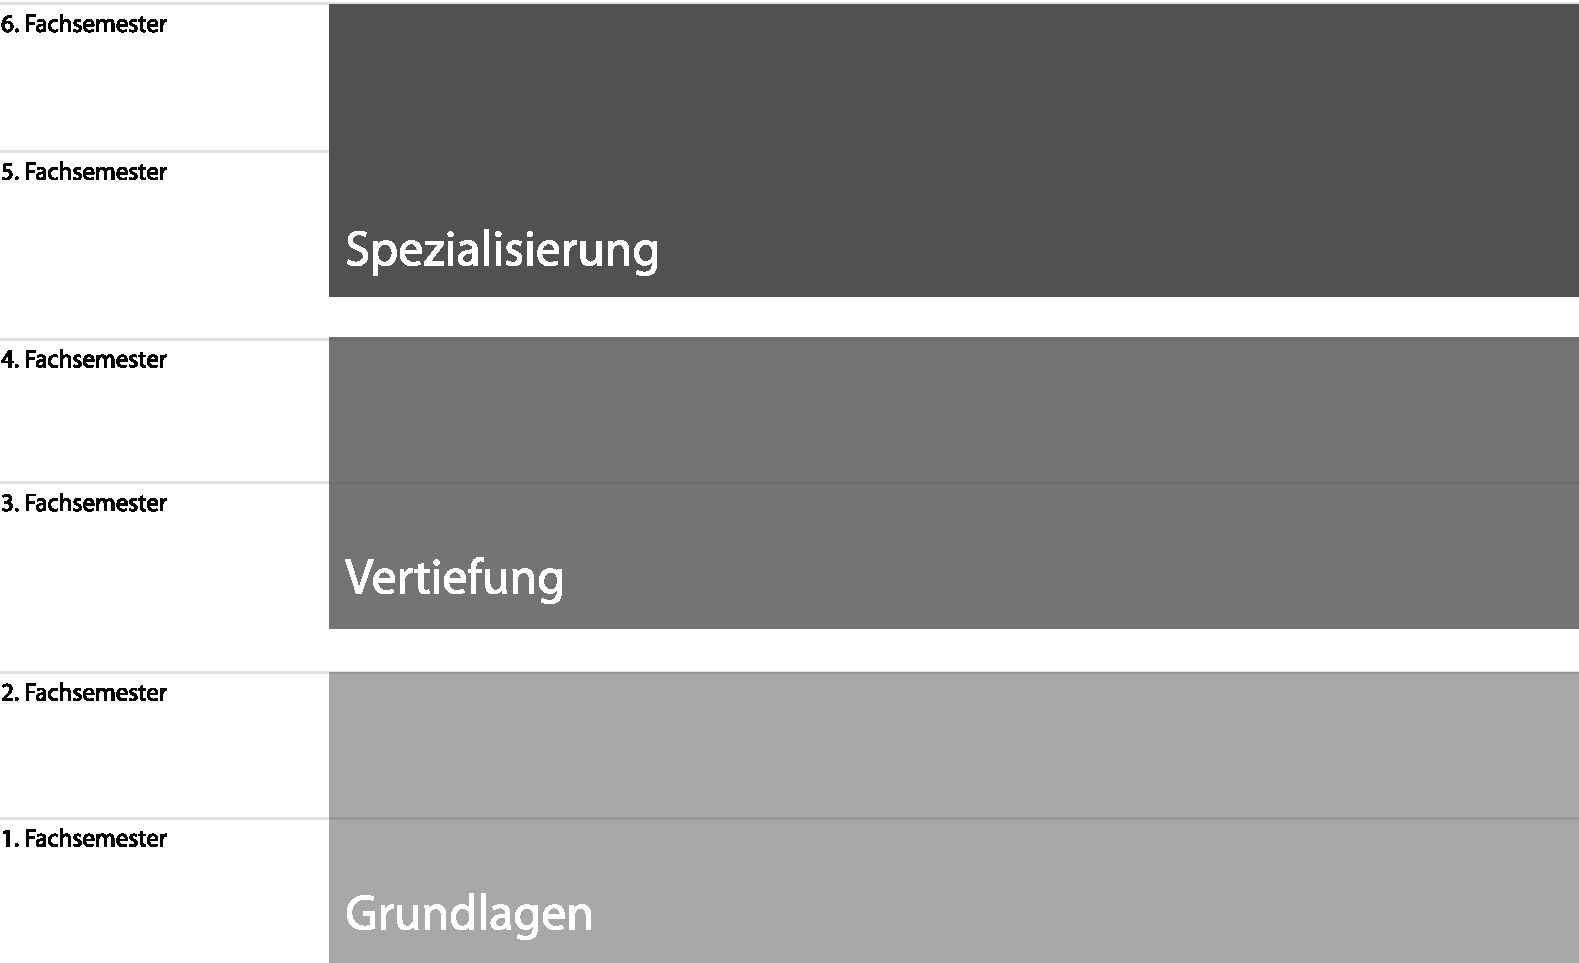
\includegraphics[width=\columnwidth]{../anhaenge/bilder/ba-studienphasen.pdf}
\caption{Abbildung: Studienphasen des Bachelorstudiengangs
Medieninformatik}
\end{figure}

Die organisatorischen und inhaltliche Klammer bilden die drei,
aufeinander aufbauenden, Studienphasen: Grundlagen, Vertiefung und
Spezialisierung. Die Module innerhalb der Phasen, gliedern sich in zwei
Säulen: Informatik Kernmodule und Medieninformatik-spezifische Module.
Die Informatik Kernmodule auch von anderen Informatik Studiengängen der
Fakultät 10 genutzt. Dadurch werden Synergien erzeugt und alle
Informatik Studenten der Fakultät können auf die gleiche Wissensbasis
zurückgreifen. Durch die Durchmischung von Studierenden
unterschiedlicher Studiengänge können hier unter den Studierenden
bereits interdisziplinäre Kontakte geknüpft werden. Ein weiterer Vorteil
dieser Konstruktion ist eine gute Durchlässigkeit von Studierenden beim
Studiengangswechsel, sofern sie feststellen, dass ein anderer
Studiengang am Campus eher ihren Fähigkeiten und Neigungen entspricht.
Naturgemäß die Informatik Kernmodule, die zumeist Grundlagencharakter
haben, im Grundlagenteil des Studiums verankert.

Um den Studierenden jedoch mit den Herangehensweisen und Perspektiven
der Medieninformatik möglichst früh vertraut zu machen und sie bei der
Identifikation mit der Domäne zu unterstützen, wir im ersten Semester
das Modul ``Einführung in die Medieninformatik'' mit einem Gewicht von
10 Creditpoints angeboten. Im zweiten Semester übernimmt das Modul
``Mensch-Computer Interaktion'' mit einem Gewicht von 10 Creditpoints
diese Aufgabe. Das Gewicht der Medieninformatik-spezifischen Module
nimmt mit jedem Semester zu.

\subsection{Sinnvolle Staffelung der
Module}\label{sinnvolle-staffelung-der-module}

\begin{figure}[htbp]
\centering
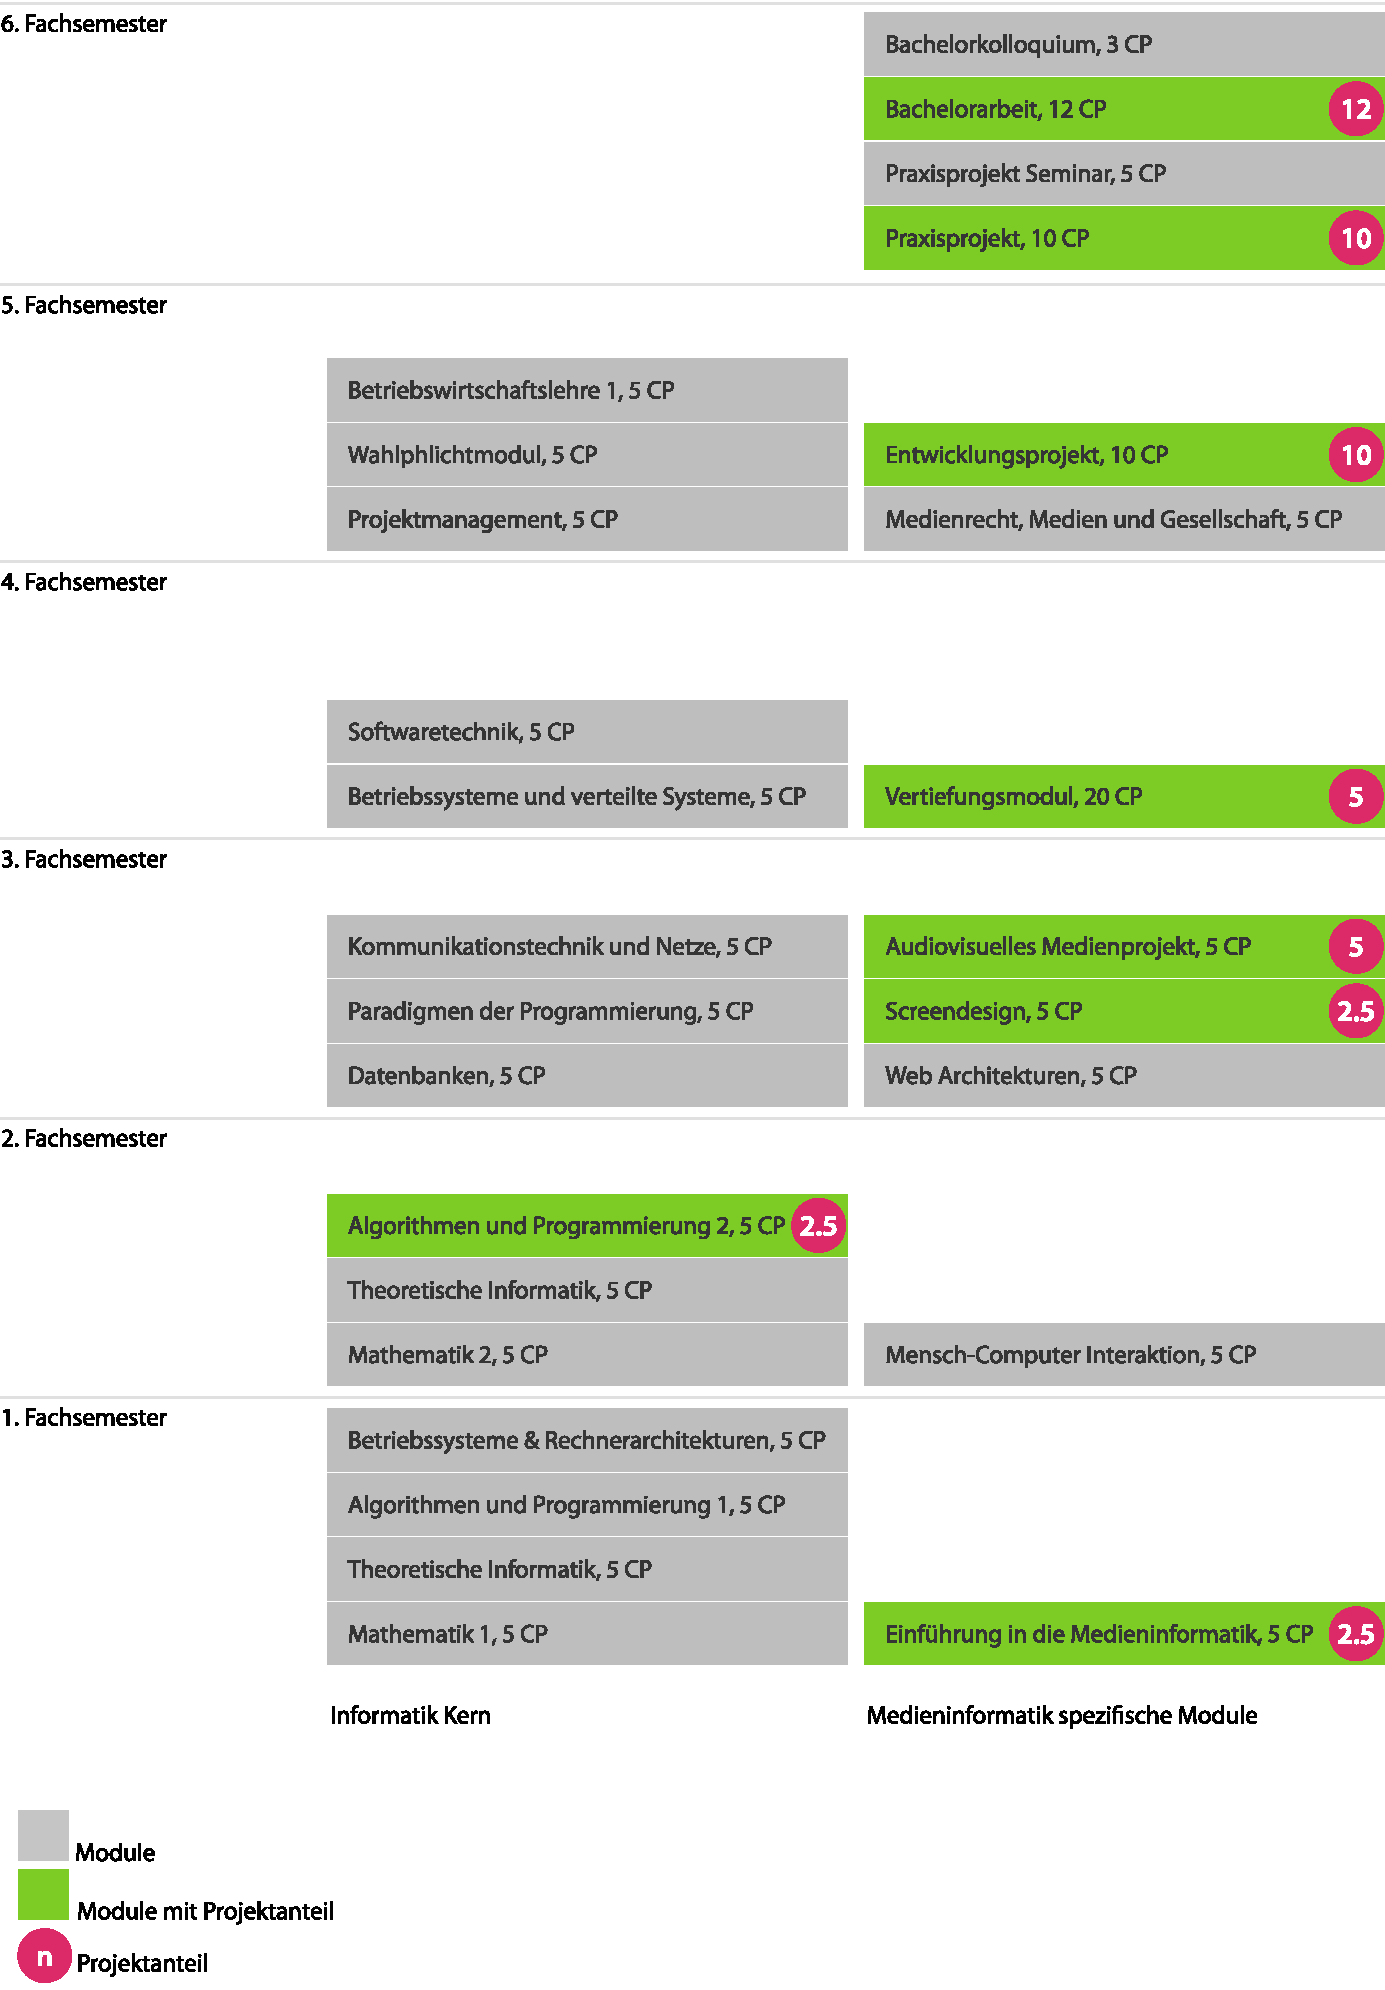
\includegraphics[width=\columnwidth]{../anhaenge/bilder/ba-verlaufsplan.pdf}
\caption{Abbildung: Studienverlaufsplan des Bachelorstudiengangs
Medieninformatik}
\end{figure}

Die ersten Modulen des Informatik Kerns bauen vor allem mathematische,
algorithmische und und grundlegende Kenntnisse und Fertigkeiten auf. Im
Kontrast dazu, werden im Modul ``Einführung in die Medieninformatik''
vielfältige Perspektiven, Konzepte und Arbeitstechniken der
Medieninformatik, quasi im Vorgriff auf der kommende Studium,
vorgestellt und in einem Projekt, mit forschendem Charakter, angewendet.
Hiermit wird den Studierenden ein Ausblick auf das weitere Studium und
die notwendigen Arbeitsweisen und -techniken gegeben.

Im weiteren Studienverlauf sind die Medieninformatik-spezifischen Module
an den groben Phasen der Produktentwicklung ausgerichtet: Konzeption,
Realisierung und Reflexion ausgerichtet. Die Module ``Mensch-Computer
Interaktion'', ``Screendesign'' und ``Web-Architekturen'' vermitteln
überwiegend Herangehensweisen, Techniken und Konzepte für die
Konzeptionsphase eines Projekts. Das Modul ``Audiovisuelles
Medienprojekt'' adressiert sowohl Themen rund um die Konzeption als auch
in Richtung Projektrealisierung und bildet den Übergang zum
Vertiefungsmodul im vierten Semester, in dem Realisierungsaspekte im
Vordergrund stehen.

Mit dem ``Entwicklungsprojekt'' im fünften Semester werden zunehmend
Fragestellung und Herangehensweisen zur Reflexion eines Projekts, z.B.
als Vorbereitung einer weiteren Projektiteration, fokussiert.

Um den Studierende fundierte Entwicklungskompetenz zu vermitteln, wird
ein Modulstrang aus dem Informatik Kern verwendet, der ausgehend den
Prinzipien der Objektorientierung und einfachen Algorithmen (Algorithmen
und Programmierung 1) über komplexere Prinzipien der
Algorithmenentwicklung (Algorithmen und Programmierung 2) hin zu
Anwendung unterschiedlicher Programmierkonzepte (Paradigmen der
Programmierung) und Prinzipien, Methoden und Techniken der
modellbasierten Softwareentwicklung (Softwareentwicklung) diese
Kompetenz sukzessive auf- und ausbaut.

\subsection{Individuelle
Vertiefungsmöglichkeiten}\label{individuelle-vertiefungsmuxf6glichkeiten}

Im vierten Semester wird zur Fachvertiefung entsprechen der persönlichen
Neigung ein Vertiefungsmodul mit einem Gewicht von 20 Creditpoints
angeboten. Hier stehen drei Vertiefungsrichtungen zur Auswahl: Visual
Computing, Social Computing und Web-Development. Die Studierenden haben
in diesem Modul die Möglichkeit, entsprechend der persönlichen Neigung,
ein Themenfeld tief zu durchdringen und damit eine
Spezialisierungsrichtung vorzubereiten. Durch das Zusammenfassen
mehrerer Module werden im Vertiefungsmodul konsistente Regularien, sowie
inhaltliche und organisatorische Zusammenhänge geschaffen.

Das Entwicklungsprojekt im fünften Semester bietet die Möglichkeit zur
weiteren Fachvertiefung entsprechend der persönlichen Neigungen. Im
gleichen Semester ist Wahlpflichtmodul verankert, bei dem ein Modul aus
dem Wahlkatalog der Informatik, oder ein Pflichtmodul eines anderen
Informatik Studiengangs der Fakultät gewählt werden kann.

Zusammen mit dem Praxisprojekt und der Bachelorarbeit stehen somit 60
Creditpoints, also ein Drittel der Studienleistungen, zur individuellen
Fachvertiefung zur Verfügung.

\subsection{Projektorientierung und Aufbau der
Projektgrößen}\label{projektorientierung-und-aufbau-der-projektgruxf6uxdfen}

Projektorientierung und forschendes Lernen sind seit der
Erstakkreditierung des Studiengangs elementare Bestandteile des
Studienkonzepts. Diese Ansätze haben in den letzten Jahren vermehrt
Einzug in verschiedene Module erhalten. Um hier die Studierenden
einerseits nicht zu überfordern, sie aber aber trotzdem an größere und
komplexere Projekte und Fragestellungen heranzuführen, werden die
Projektanteile und -gewichte im Studiengang behutsam aufgebaut. Das
Module ``Einführung in die Medieninformatik'' startet im ersten Semester
mit einem Projektanteil von 50\% (2,5 CP) um die Studierenden initial
mit dem Lehrformat ``Projekt'' im Hochschulkontext vertraut zu machen.
Das Gewicht der Projekte wird dann im dritten und vierten Semester auf 5
Creditpoints erhöht. Das Modul ``Entwicklungsprojekt'' im fünften
Semestern ist mit einem Gewicht von 10 Creditpoints ausgestattet und
leitet über zum Praxisprojekt (10 CP) und der Bachelorarbeit (12 CP).
Das Projektgewicht von 12 Creditpoints wird später, im konsekutiven
Masterstudiengang, weiter geführt.

\subsection{Wissenschaftliches
Arbeiten}\label{wissenschaftliches-arbeiten}

Wissenschaftliches Arbeiten wird beginnend im ersten Semester in der
Veranstaltung ``Einführung in die Medieninformatik'', in der THemen wie
Recherche, Umgang mit Quellen, adäquater Aufbau von Dokumenten und
Verwendung adäquater Sprache thematisiert und gefordert wird. Darauf
wird u.a. in allen Projektorientierten Veranstaltungen bei der
Erstellung von Projektdokumentationen, bei Vorträgen und bei Poster
Präsentationen zurück gegriffen. Im Rahmen des Praxisprojekt Seminars
wird das Thema im Hinblick auf die anschließende ERstellung der
Bachelorarbeit vertieft und eine eingehende individuelle
Auseinandersetzung mit dem Thema abgerufen.

\subsection{Weiterführende
Dokumente}\label{weiterfuxfchrende-dokumente-2}

\begin{itemize}
\tightlist
\item
  Themen der Abschlussarbeiten von 2010 bis 2014\footnote{Themen der
    Abschlussabeiten des Medieninformatik Bachelor 2010 bis 2014:
    \href{../anhaenge/abschlussarbeiten_2010-2014_.pdf}{abschlussarbeiten\_2010-2014\_.pdf}}
\item
  Studienverlaufsplan Medieninformatik Bachelor\footnote{Studienverlaufsplan
    Medieninformatik Bachelor fehlt}
\item
  Modulhandbuch Medieninformatik Bachelor\footnote{Modulhandbuch
    Medieninformatik Bachelor fehlt}
\item
  Ziele-Module-Matrix Medieninformatik Bachelor\footnote{Ziele-Module-Matrix
    Medieninformatik Bachelor:
    \href{../anhaenge/Ziele-Module-Matrix-Medieninformatik-Bachelor.pdf}{Ziele-Module-Matrix-Medieninformatik-Bachelor.pdf}
    (abgerufen am 13.02.2017)}
\end{itemize}

\section{Master}\label{master}

Der viersemestrige Masterstudiengang baut konsekutiv auf das
Bachelorprogramm auf. Im Gegensatz zum Bachelorstudium, sind hier
Einschreibungen im Sommer- und Wintersemester möglich. Dies führt zu
unterschiedlichen Studienverlaufplänen in Abhängigkeit des
Einschreibesemesters.

\subsection{Studienschwerpunkte}\label{studienschwerpunkte}

\begin{figure}[htbp]
\centering
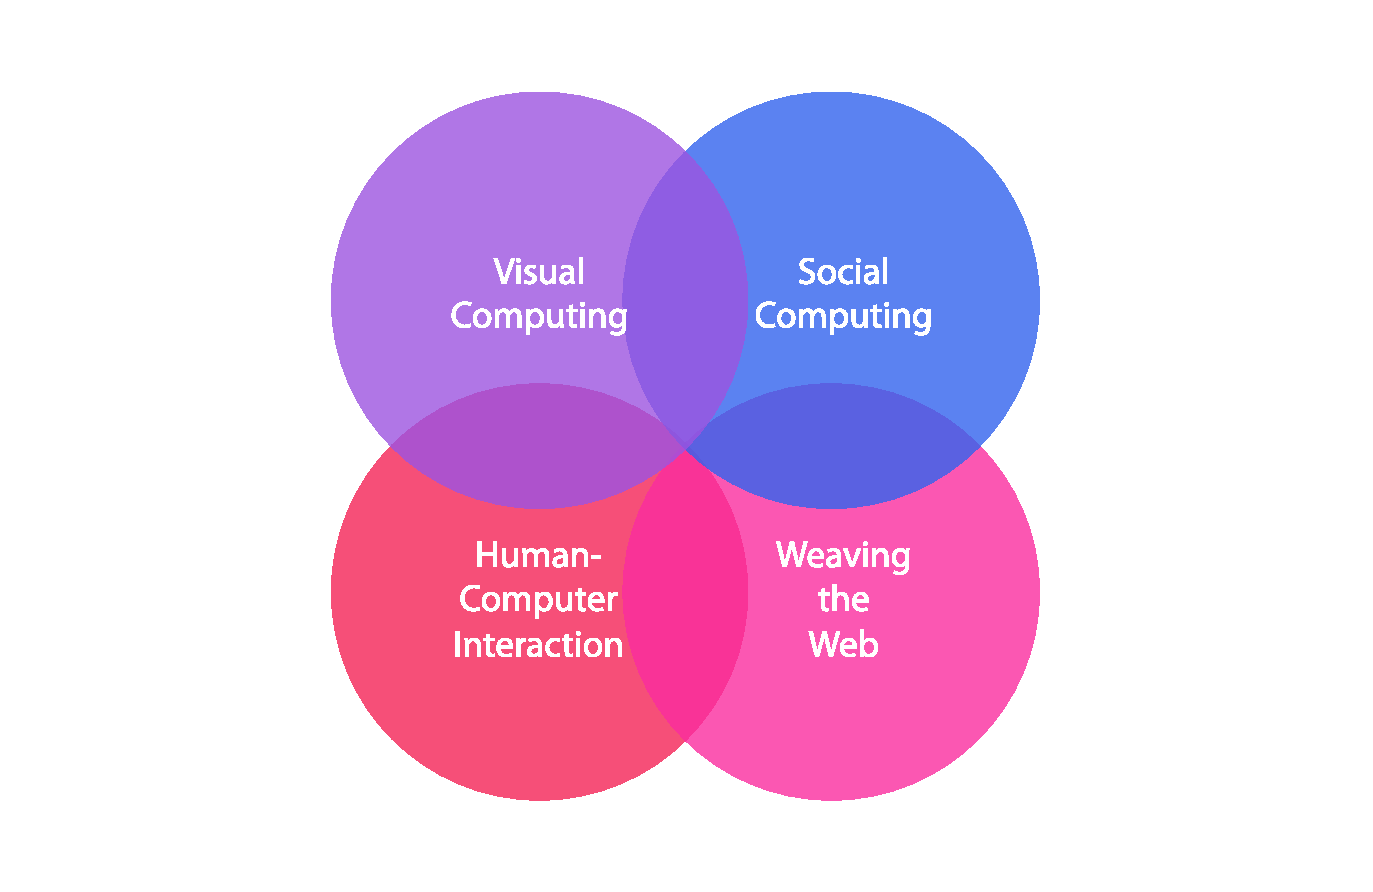
\includegraphics[width=\columnwidth]{../anhaenge/bilder/ma-schwerpunkte.pdf}
\caption{Abbildung: Schwerpunkte Medieninformatik Master}
\end{figure}

Zur individuellen Schwerpunktbildung bietet des Masterprogramm vier
Möglichkeiten, die alle auf den im Bachelor gelegten Themenbieten
aufbauen: Human-Computer Interaction, Social Computing, Visual Computing
und Weaving the Web. Für Studierende, die ein generalistisch geprägtes
Studium bevorzugen wird der Studienpfad ``Multiperspective Product
Development'' angeboten, der sich aus ausgewählten Modulen der anderen
Schwerpunkte und des Wahlplichtkatalogs speist. Dieser wird aus
organisatorischen Gründen auch als Schwerpunkt aufgeführt.

\subsection{Studienphasen und
-säulen}\label{studienphasen-und--suxe4ulen-1}

\begin{figure}[htbp]
\centering
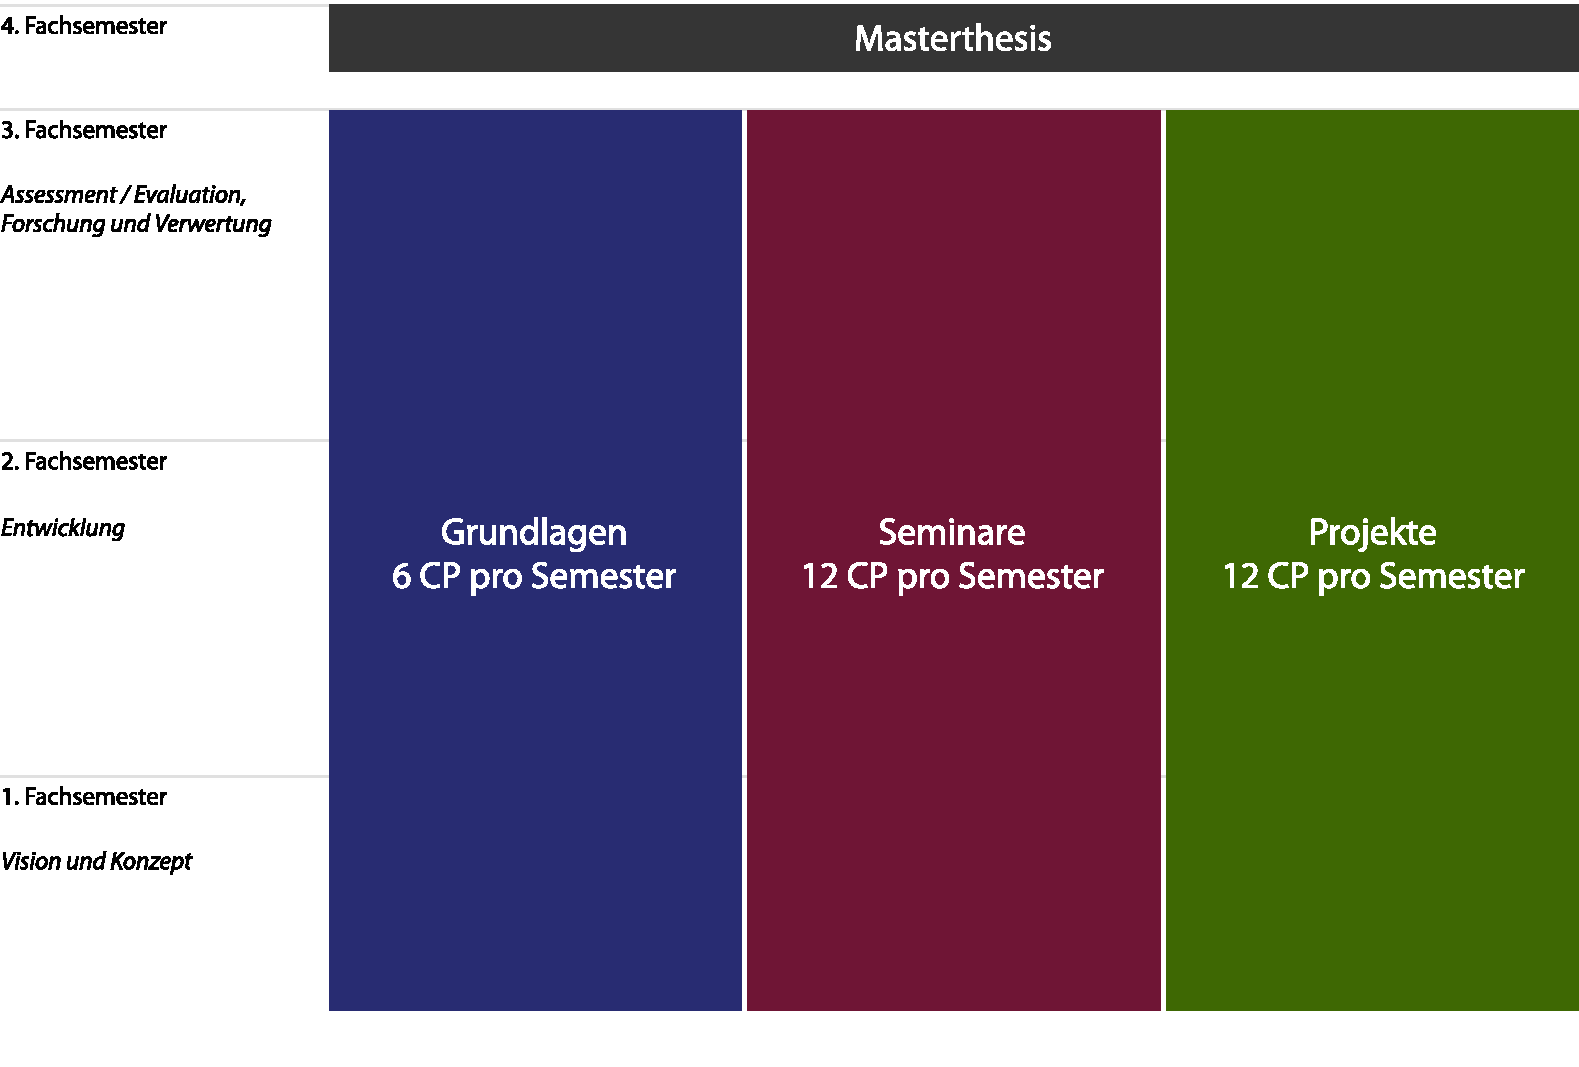
\includegraphics[width=\columnwidth]{../anhaenge/bilder/ma-saeulen.pdf}
\caption{Abbildung: Elemente des Masterprogramms bei Studienstart im
Wintersemester}
\end{figure}

Jedes der ersten drei Fachsemester steht unter einer übergreifenden
Leitfrage. Diese Fragen sind, ähnlich wie im Bachelorprogramm, am groben
Ablauf der Produktentwicklung ausgerichtet: ``Vision \& Konzept'',
``Entwicklung'' und ``Assessment/Evaluation, Forschung und Verwertung''.
Die Leitfragen sind vor allem für die Projekte relevant. Das vierte
Fachsemester wird komplett von der Masterthesis ausgefüllt.

Die ersten beiden Studiensemester setzen sich aus drei strukturierenden
Elementen zusammen: Kernmodule, Schwerpunktmodule und Projekt. Die
Kernmodule ``Spezielle Gebiete der Mathematik'', ``Computerethik'' und
``Research Methods'' sind für alle Studierende des Studienprogramms
verbindlich, wogegen die Schwerpunktmodule abhängig vom jeweiligen
Schwerpunkt sind.

Im dritten Semester können die Studierenden drei Module aus dem Katalog
aller Module der Informatik Masterstudiengänge der Fakultät wählen und
damit ihre Studieninhalte entsprechend ihres Schwerpunkts und der
persönlichen Neigung ausprägen.

\begin{figure}[htbp]
\centering
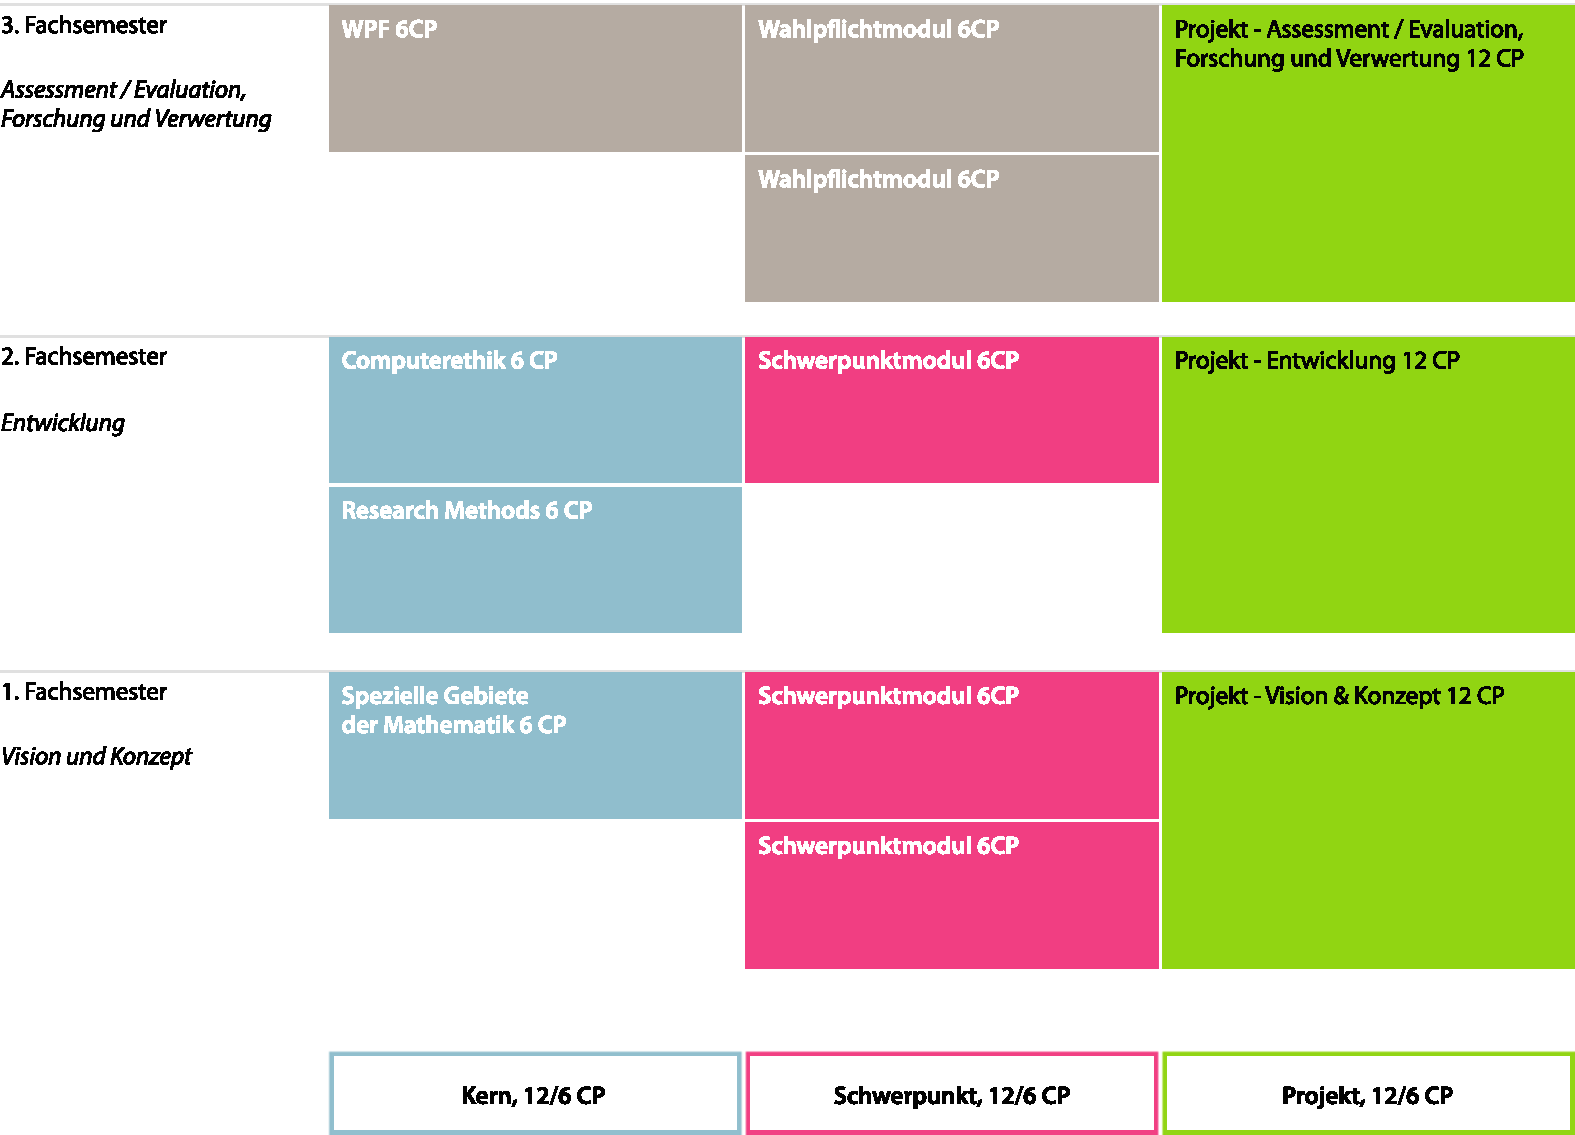
\includegraphics[width=\columnwidth]{../anhaenge/bilder/ma-struktur.pdf}
\caption{Abbildung: Struktur der ersten drei Studiensemester des
Masterprogramms bei Studienstart im Wintersemester}
\end{figure}

Jedes der ersten drei Fachsemester hat ein dezidiertes Projekt, das auf
die jeweilige Leitfrage ausgerichtet ist. An den Projekten können
Studierende aus den verschiedenen Schwerpunkten teilnehmen, um hier eine
Fragestellung gezielt aus verschiedenen Perspektiven zu beleuchten. Der
Grundgedanke ist, dass in jedem Semester nur die Phase der
entsprechenden Leitfrage durchlaufen und so abgeschlossen und
aufbereitet wird, das im nächsten Semester oder zu einem späteren
Zeitpunkt eine anderes Team auf den Ergebnissen aufsetzen kann. Diese
Herangehensweise hat folgende Vorteile: - Bearbeitung von komplexen
(Forschungs-) Fragestellungen - Erleben und Einüben von sequentiellen
arbeitsteiligen Prozessschritten - Sensibilisierung für professionelle
Ergebnissicherung - Skalierbarkeit von Projekten auf verschiedene Teams
in Abhängigkeit von der jeweiligen Projektphase

Die Projekte können mit zusätzlichen Lehrveranstaltungen, die auf die
jeweilige Leitfrage einzahlen, angereichert werden.

\subsection{Wissenschaftliches
Arbeiten}\label{wissenschaftliches-arbeiten-1}

Die Fortsetzung des Masterstudiengang durch ein Promotionsstudium ist
eine Möglichkeit, die von einer erheblichen Anzahl unserer Absolventen
wahrgenommen wird. Um dafür die erforderlichen Kompetenzen im
wissenschaftlichen Arbeiten zu erreichen aber auch um Interesse am
wissenschaftlichen Arbeiten zu wecken, wird dieses Thema im Master
konsequent verfolgt. Neben expliziten, auf Vermittlung von
Methodenwissen ausgelegten Modulen wie ``Research Methods'' und
``Computer Ethik'' wird vor allem in den Schwerpunktprojekten
wiisenschaftliches Arbeiten gefordert. Im Projektteil ``Vision und
Konzept'' wird im Rahmen der Veranstaltung ``Advanced Seminar'' wird
Aquisition, Bewertung und Erschließung des aktuellen Forschungsstandes
aus wissenschaftlicher Literatur thematisiert. Im Projektteil
``Umsetzug'' wird eine kritische Diskussion der eingesetzten Methoden
und Architekturen praktiziert. Im Projektteil ``Verwertung'' wird auch
die Publikation der Ergebnisse auf Konferenzen, Workshops, oder in
sozialen Medien wit github angestrebt.

\subsection{Internationalisierung}\label{internationalisierung}

Die inhaltliche Offenheit des dritten Fachsemesters mit drei
Wahlpflichtmodulen und einem Projekt ermöglicht den Studierenden ein
Auslandssemester, da hier die Anrechnung von Studienleistung problemlos
möglich ist.

\subsection{Weiterführende
Dokumente}\label{weiterfuxfchrende-dokumente-3}

\begin{itemize}
\tightlist
\item
  Studienverlaufsplan Medieninformatik Master\footnote{Studienverlaufsplan
    Medieninformatik Master fehlt}
\item
  Modulhandbuch Medieninformatik Master\footnote{Modulhandbuch
    Medieninformatik Master fehlt}
\item
  Prüfungsordnung Medieninformatik Master(entwurf)\footnote{Prüfungsordnung
    Medieninformatik Master(entwurf):
    \href{../anhaenge/MIMPO_Entwurf_ohne_Anm_Sz20170218.pdf}{MIMPO\_Entwurf\_ohne\_Anm\_Sz20170218.pdf}}
\item
  Ziele-Module-Matrix Medieninformatik Master\footnote{Ziele-Module-Matrix
    Medieninformatik Master fehlt}
\end{itemize}

\chapter{Studierbarkeit}\label{studierbarkeit}

\begin{quote}
Die Studierbarkeit des Studiengangs wird gewährleistet durch:

\begin{itemize}
\tightlist
\item
  die Berücksichtigung der erwarteten Eingangsqualifikationen,
\item
  eine geeignete Studienplangestaltung
\item
  die auf Plausibilität hin überprüfte (bzw. im Falle der
  Erstakkreditierung nach Erfahrungswerten geschätzte) Angabe der
  studentischen Arbeitsbelastung,
\item
  eine adäquate und belastungsangemessene Prüfungsdichte und
  -organisation,
\item
  entsprechende Betreuungsangebote sowie
\item
  eine fachliche und überfachliche Studienberatung.
\end{itemize}

Die Belange von Studierenden mit Behinderung werden berücksichtigt.

\textbf{Leitfragen}

\begin{itemize}
\item
  Woran erkennen die Verantwortlichen, dass die (formalen und
  fachlich-inhaltlichen) Zugangskriterien das Erreichen des angestrebten
  Kompetenzprofils unterstützen?
\item
  Ggf.: Wie wurde reagiert, wenn die Zugangsregelungen diesen Zweck aus
  Sicht der für den Studiengang Verantwortlichen nicht erfüllt haben?
\item
  Wie schätzen die für den Studiengang Verantwortlichen und daran
  Beteiligten -- einschließlich der Studierenden -- die studentische
  Arbeitsbelastung ein? Welche Probleme treten auf? Was wird zu deren
  Lösung unternommen?
\item
  Sind hinsichtlich des Studienabschlusses in der vorgesehenen Zeit in
  den vergangenen Jahren Probleme aufgetreten? Wenn ja, welche? Wie
  wurden sie behandelt?
\item
  Inwieweit sind individuelle Mobilitätsfenster für Studierende im
  Studienverlauf realisierbar? Welche Probleme gibt es? Wie wurde darauf
  reagiert?
\item
  Welche Auswirkungen auf die Studierbarkeit haben die vorhandenen
  (prüfungsrelevanten) Regelungen zu Wiederholungsmöglichkeiten,
  Nachteilsausgleich bei Behinderung, Nichterscheinen im Krankheitsfall
  etc.?
\item
  Gab es Fälle, in denen sich die konkrete Prüfungsorganisation (z.~B.
  Terminierung der Prüfungen, Korrekturzeiten) nachteilig auf den
  Studienverlauf ausgewirkt haben? Wenn ja, welche Konsequenzen wurden
  gezogen?
\item
  Welche der vorhandenen Betreuungs- und Beratungsangebote für
  Studierende halten die für den Studiengang Verantwortlichen und
  Beteiligten -- einschließlich der Studierenden -- für besonders
  effektiv im Hinblick auf den Studienerfolg?
\item
  Welche Betreuungs- und Beratungsangebote für Studierende vermissen die
  für den Studiengang Verantwortlichen und Beteiligten -- einschließlich
  der Studierenden? Warum werden sie nicht realisiert?
\item
  Inwieweit werden Belange von Studierenden mit Behinderung
  berücksichtigt?
\end{itemize}

\textbf{Mögliche Evidenzen}

\begin{itemize}
\item
  Ggf. Zugangssatzung sowie Informationen über die
  Studiengangsvoraussetzungen auf Webseiten, in Studienführern etc.
\item
  Einschlägige Ergebnisse interner Erhebungen und Evaluationen -- ggf.
  Daten zur studentischen Arbeitslast
\item
  Studienverlaufsplan, aus der/dem Semesterlage, Umfang und studentische
  Arbeitslast der Module pro Semester hervorgehen (ggf. mit
  Veröffentlichungsort wie z.~B. Homepage, Studienführer, Studien- bzw.
  Prüfungsordnungen) bzw. Dokumente, in denen Studienverläufe und deren
  Organisation geregelt sind
\item
  Dokumente, aus denen die geltenden Regelungen zur
  (Auslands-)Mobilität, Praxisphasen und Anerkennung von an anderen
  Hochschulen / außerhalb der Hochschule erbrachten Leistungen erkennbar
  sind
\item
  Dokumente aus dem täglichen Gebrauch an der Hochschule, aus denen das
  vorhandene Beratungs- und Betreuungskonzept hervorgeht
\item
  (Statistische) Daten zu Studienverläufen
\item
  Ggf. Daten zur (Auslands-)Mobilität von Studierenden und zu
  Praxiseinsätzen von Studierenden
\item
  Ggf. weitere einschlägige Ergebnisse interner Befragungen und
  Evaluationen (auch Auffälligkeiten hinsichtlich der Wirkung von ggf.
  vorhandenen Maßnahmen zur Vermeidung von Ungleichbehandlungen in der
  Hochschule)
\end{itemize}
\end{quote}

\section{Bachelor
Medieninformatik}\label{bachelor-medieninformatik-1}

\subsection{Zugangsvoraussetzungen}\label{zugangsvoraussetzungen}

Als Voraussetzung für die Aufnahme eines Bachelorstudiums
Medieninformatik wird die Fachhochschulreife oder eine als gleichwertig
anerkannte Vorbildung gefordert. Für die nächste Einschreibephase wurde
darüber hinaus eine Zulassungsbeschränkung für alle Informatik
Bachelorstudiengänge vereinbart.

\begin{verbatim}
cn: wie wird das denn korrekt formuliert?
\end{verbatim}

\subsection{Allgemeine/fachgebundene Hochschulreife,
Fachhochschulreife, einschlägige
Berufserfahrung}\label{allgemeinefachgebundene-hochschulreife-fachhochschulreife-einschluxe4gige-berufserfahrung}

Voraussetzung für den Zugang zum Bachelorstudium ist die
Fachhochschulreife oder eine als gleichwertig anerkannte Vorbildung.

\subsection{Praktika/Berufserfahrung}\label{praktikaberufserfahrung}

keine

\subsection{Fremdsprachenkenntnisse,
Deutschkenntnisse}\label{fremdsprachenkenntnisse-deutschkenntnisse}

Fremdsprachenkenntnisse, die über das Maß der durch den schulischen
Abschluss gegebenen Fremdsprachenkenntnisse hinausgehen, sind nicht
gefordert. Die Deutschkenntnisse ausländischer Studierender werden
i.d.R. durch Ablegen der Deutschen Sprachprüfung für den Hochschulzugang
(DSH II) oder eine äquivalente Prüfung nachgewiesen; für nähere
Informationen sowie Einzelfallregelungen ist das International Office
der TH Köln zuständig\footnote{International Office fehlt}.

\subsection{Eignungsfeststellung}\label{eignungsfeststellung}

Keine

\section{Master Medieninformatik}\label{master-medieninformatik-1}

Als Voraussetzung für die Aufnahme des Studiums wird ein Bachelor oder
Diplom- Abschluss einer deutschen Fachhochschule oder Universität in
Informatik oder ein gleichwertiger Abschluss gefordert. Liegt ein
anderer Hochschulabschluss vor, so können die Voraussetzungen für das
Studium auch durch eine einschlägige Berufspraxis von in der Regel
mindestens zwei Jahren in einem für die Medieninformatik relevanten
Tätigkeitsfeld erbracht werden. Bei Vorliegen eines anderen
Hochschulabschlusses als oben festgelegt, müssen durch die Berufspraxis
Qualifikationen in Informatik erworben worden sein, die den
Qualifikationen eines Bachelorabsolventen in Informatik äquivalent sind.
Eine vom Prüfungsausschuss benannte Kommission, bestehend aus zwei
Professoren oder Professorinnen der Fakultät für Informatik und
Ingenieurwissenschaften, entscheidet, ob bei dem Bewerber oder der
Bewerberin die für die Aufnahme des Studiums notwendigen fachlichen
Qualifikationen vorliegen.

\section{Struktur}\label{struktur}

Im Anhang K sind die Studienverlaufspläne der einzelnen Studiengänge
enthalten, für die eine Akkreditierung beantragt wird. Das Studium
umfasst im Bachelor jeweils insgesamt 180 ECTS Punkte und 144
Semesterwochenstunden Semesterwochenstunden. Dies entspricht
durchschnittlich 24 SWS je Semester. Die Inhalte der Module sind in dem
entsprechenden Modulhandbuch dargestellt.

Das Masterstudium umfasst 120 ECTS Punkte bei 48 SWS Präsenzzeit, was
einer durchschnittlichen Präsenzzeit von 16 SWS pro Semester entspricht.

\section{Arbeitslast}\label{arbeitslast}

Die Bachelor- und Masterstudiengänge sind durchgängig mit 30
ECTS-Punkten im Semester durchkalkuliert, was einer Arbeitslast von 900
Stunden pro Semester entspricht. Wenn man ein Semester mit 24 Wochen
veranschlagt, wobei die Prüfungszeit und Prüfungsvorbereitung
mitgerechnet ist, ergibt sich eine Wochenarbeitszeit von 900 h / 24 =
37,5 Stunden. Eine Veranstaltung mit 5 Creditpoints und 4 SWS, 2 SWS
Vorlesung + 2 SWS übung hat in der Regel einen Arbeitsaufwand von 5 x 30
= 150 Stunden. Bei durchschnittlich 18 Semesterwochen entspricht dies
einem Anteil von 2 h x 18 = 36 Stunden Vorlesung, 2 h x 18 = 36 Stunden
Übung, also 72 Stunden Präsenzanteil und 78 Stunden Selbststudium
inklusive Klausurvorbereitung und Nachbereitung der Präsenzanteile. Dies
entspricht in etwa einer Aufteilung der Gesamtzeit in 50\% für
Präsenzstudium und in 50 \% für Selbststudium.

Die Lehrveranstaltungen des Masterstudiengangs sind mit 6 Creditpoints
ausgestattet, was bei einem Modul mit 4 SWS einem Verhältnis von 40\%
für Präsenzstudium und 60 \% für Selbststudium entspricht.

\section{Leistungspunktesystem}\label{leistungspunktesystem}

Die Module der beantragten Studiengänge werden mit ECTS-Punkten
bewertet, um europaweite Vergleichbarkeit gemäß den Bologna-Richtlinien
zu ermöglichen.

\section{Prüfungen}\label{pruxfcfungen}

Viele Fachprüfungen der Bachelorstudiengänge, vor allem der
Grundlagenfächer, werden in Form einer Klausur angeboten. Bei vielen
Pflichtmodulen, den meisten Wahlpflichtfächer und natürlich im
Kolloquium zur Bachelorarbeit sind mündliche Prüfungen vorgesehen, die
oft durch Referate und Präsentationen unterstützt werden. Die Anzahlen
der Modulprüfungen liegen bei den Bachelorstudiengängen zwischen 28 und
30 und sind so über die sechs Semester verteilt, dass es zu keinen
Häufungen mit mehr als sechs Prüfungen in einem Semester kommt.

Im Masterstudium ist der Schwerpunkt der Prüfungsformen in Richtung
mündlicher Prüfungen, Präsentationen und wissenschaftlicher
Ausarbeitungen gelegt. Bei einer Gesamtzahl von 15 Modulprüfungen fallen
maximal fünf Prüfungen pro Semester an.

\section{Studien/Prüfungsordnungen}\label{studienpruxfcfungsordnungen}

Die Studien- und Prüfungsordnungen\footnote{Link zur online
  Prüfungsordnung fehlt} der laufenden Studiengänge sind dem Anhang
dieses Berichts beigefügt. Sie sind außerdem über die Website der
Hochschule abrufbar. Der Studienverlaufsplan entspricht der
Studienordnung. Nach Zustimmung der Gutachter zu den in den erläuterten
Änderungen im Rahmen der Reakkreditierung werden die überarbeiteten
Prüfungsordnungen, bzw. Studienverlaufspläne zeitnah vorgelegt.

\section{Diploma Supplement}\label{diploma-supplement}

Das Diploma Supplement der zur Reakkrediterung beantragten Studiengänge
ist im Anhang des Dokuments zu finden.

\section{Maßnahmen zur Beratung von Studieninteressierten und
Studierenden}\label{mauxdfnahmen-zur-beratung-von-studieninteressierten-und-studierenden}

Die Medieninformatik beteiligt sich an folgenden Veranstaltungen zur
Beratung von Studieninteressierten:

Regelmäßig wird im Mai ein „Schnupperstudium`` durchgeführt, an dem rund
150 Schüler, teilweise mit ihren Lehrern teilnehmen, um die
Fachhochschule kennen zu lernen.

Das Medieninformatik beteiligt sich regelmäßig mit eigenen
Veranstaltungen an dem bundesweit jährlich stattfindenden Girls-Day, an
dem rund 50 Schülerinnen speziell für ein Informatik-Studium oder ein
ingenieurwissenschaftliches Studium in Gummersbach begeistert werden
sollen.

Dazu kommen Laborführungen für Schülergruppen verschiedener Schulen
sowie die Präsentation des Campus Gummersbach außerhalb der Hochschule:
- auf der „Overather Ausbildungsbörse``, - der „Ausbildungsbörse
Bergneustadt'', - der „Mädchenmesse" des Oberbergischen Kreises, - dem
„Tag der Offenen Tür" des Berufskollegs Dieringhausen (Gummersbach),der
„Weiterbildungsmesse Oberberg``, - sowie die Teilnahme an anderen,
unregelmäßig durchgeführten Veranstaltungen zur Studien- und Berufswahl.

Das Institut für Informatik beteiligt sich jährlich am „Tag der offenen
Tür`` der TH-Köln im September und an Informationsveranstaltungen der
umliegenden Gymnasien und anderer weiterführender Schulen, die
potenzielle Studienanfängerinnen und Studienanfänger an die
Qualifizierung für ein Hochschulstudium heranführen. Alle diese Angebote
werden sehr gut aufgenommen und sind stark frequentiert.

Darüber hinaus bietet die Medieninformatik einige Veranstaltungen (siehe
außercurriculare Maßnahmen) wie den jährlichen Showcase an, um hier auch
eine Plattform für Studieninteressierte zu schaffen. Diese Angebote
werden gut angenommen.

\chapter{Prüfungssystem}\label{pruxfcfungssystem}

\begin{quote}
Die Prüfungen dienen der Feststellung, ob die formulierten
Qualifikationsziele erreicht wurden. Sie sind modulbezogen sowie
wissens- und kompetenzorientiert. Jedes Modul schließt in der Regel mit
einer das gesamte Modul umfassenden Prüfung ab. Der Nachteilsausgleich
für behinderte Studierende hinsichtlich zeitlicher und formaler Vorgaben
im Studium sowie bei allen abschließenden oder studienbegleitenden
Leistungsnachweisen ist sichergestellt. Die Prüfungsordnung wurde einer
Rechtsprüfung unterzogen.

\textbf{Leitfragen}

\begin{itemize}
\item
  Welche der eingesetzten Prüfungsformen stufen die Lehrenden und die
  für den Studiengang Verantwortlichen als besonders geeignet zur
  Erfassung erreichter Lernergebnisse ein? Welche Lernergebnisse lassen
  sich aus Sicht der Lehrenden und der für den Studiengang
  Verantwortlichen nur schwer überprüfen?
\item
  Wie werden die Bewertungskriterien für Studierende und Lehrende
  transparent gemacht?
\end{itemize}

\textbf{Mögliche Evidenzen}

\begin{itemize}
\item
  Prüfungsrelevante Regelungen
\item
  Einschlägige Ergebnisse aus internen Befragungen und Evaluationen mit
  Blick auf die Prüfungsorganisation und die Lernergebnisorientierung
  der Prüfungen
\item
  Beispielhafte Prüfungspläne (einschließlich Prüfungstermine)
\item
  Statistische Daten zum Studienverlauf, z.B. Durchschnittsnote,
  Durchfallquote, Anzahl der Wiederholungen
\end{itemize}
\end{quote}

\section{Studien/Prüfungsordnungen}\label{studienpruxfcfungsordnungen-1}

Die Studien- und Prüfungsordnungen der laufenden Studiengänge sind dem
Anhang G dieses Berichts beigefügt. Der Studienverlaufsplan entspricht
der Studienordnung. Nach Zustimmung der Gutachter zu den in den
Abschnitten 1 und 1 erläuterten Änderungen im Rahmen der
Reakkreditierung werden die überarbeiteten Prüfungsordnungen zeitnah
vorgelegt.

\begin{verbatim}
sm: hier stimmt noch was mit den Abschnitten nicht. Welche Abschnitte sind gemeint?
\end{verbatim}

\chapter{Studiengangsbezogene
Kooperationen}\label{studiengangsbezogene-kooperationen}

\begin{quote}
Beteiligt oder beauftragt die Hochschule andere Organisationen mit der
Durchführung von Teilen des Studiengangs, gewährleistet sie die
Umsetzung und die Qualität des Studiengangskonzeptes. Umfang und Art
bestehender Kooperationen mit anderen Hochschulen, Unternehmen und
sonstigen Einrichtungen sind beschrieben und die der Kooperation zu
Grunde liegenden Vereinbarungen dokumentiert.

\textbf{Leitfragen}

\begin{itemize}
\tightlist
\item
  Funktionieren die hochschulinternen und hochschulexternen
  Kooperationen aus Sicht der für den Studiengang Verantwortlichen?
\end{itemize}

\textbf{Mögliche Evidenzen}

\begin{itemize}
\tightlist
\item
  Kooperationsverträge, Regeln für interne/externe Kooperationen
\end{itemize}
\end{quote}

\section{Hochschulinterne
Zusammenarbeit}\label{hochschulinterne-zusammenarbeit}

\begin{verbatim}
me: Ist das folgende noch aktuell?
\end{verbatim}

\subsection{Fakultätsübergreifende
Zusammenarbeit}\label{fakultuxe4tsuxfcbergreifende-zusammenarbeit}

Innerhalb der Hochschule wird eine enge Kooperation mit einigen in Köln
angesiedelten Fakultäten gepflegt. Zu nennen sind hier vor allem die
Bereiche Design, Photoingenieurwesen, Wirtschaft,
Informationswissenschaften und Sozialwissenschaften. Mit der „Köln
International School of Design`` als interne Einrichtung der „Fakultät
für Kulturwissenschaften`` (Fakultät 02) und der „Fakultät für
angewandte Sozialwissenschaften`` (Fakultät 01) werden gemeinsame
Lehrveranstaltungen durchgeführt. Das Modul „Wissensmanagement`` des
Masterstudiengangs bspw. wird von der „Fakultät für
Wirtschaftswissenschaften`` der Fachhochschule Köln (Fakultät 04)
importiert. Das Institut für Informatik und das Institut für Automation
\& IT sind ferner im Forschungsschwerpunkt COSA (s Kap. 5.1.3.3)
synergetisch verbunden. Es besteht ein kontinuierlicher Austausch mit
dem Institut für Tropentechnologie der Fachhochschule Köln: Jährlich
wird von Herrn Prof.~Dr.~Jacksons Roehrig das Wahlpflichtfach „GIS
Geografische Informationssysteme`` angeboten.

\subsection{Fakultätsinterne
Zusammenarbeit}\label{fakultuxe4tsinterne-zusammenarbeit}

Innerhalb der Fakultät sind die Institute „Betriebswirtschaftliches
Institut Gummersbach (BIG)`` und das „Institut für Distance Learning \&
Further Education (IDF)`` mit verschiedenen Modulen in die Bachelor- und
Masterstudiengängen involviert.

Innerhalb der Fakultät 10 für Informatik und Ingenieurwissenschaften
besteht naturgemäß in der Lehre, Forschung und Entwicklung eine enge
Zusammenarbeit mit den in Gummersbach angesiedelten
ingenieurwissenschaftlichen Instituten. Dies drückt sich in einer
Vielzahl von gemeinsamen Projekten, betreuten Abschlussarbeiten sowie
einem fachübergreifenden Lehrexport und Import zwischen den beiden
Lehreinheiten aus.

\section{Externe Kooperation mit Hochschulen und
Firmen}\label{externe-kooperation-mit-hochschulen-und-firmen}

\subsection{Kooperationen mit internationalen
Hochschulen}\label{kooperationen-mit-internationalen-hochschulen}

Erste Kooperationsprojekte mit ausländischen Hochschulen datieren auf
den Beginn der 80-iger Jahre. Damals wurde eine Kooperation
(Erasmus-Kontrakt) mit der École Centrale de Lille abgeschlossen. Diese
Kooperation existiert noch heute und regelt den Austausch auf Sokrates-
und ERASMUS-Ebene von Professoren und insbesondere Studierenden.

Unter den gleichen formalen Bedingungen existiert seit vielen Jahren
eine Kooperation mit der Université Blaise Pascal in Clermont-Ferrand
und der École pour l'Informatique et les Techniques Avancées à Paris
(ÉPITA). Mit ÉPITA findet ein regelmäßiger Studierenden und
Dozentenaustausch statt; so war Herr Prof.~Hartmann (ehem. Plaßmann) im
Jahr 2006 im Rahmen einer Kurzzeitdozentur an der ÉPITA. Regelmässig
studieren ERASMUS-Studierenden von ÉPITA am Campus Gummersbach.

\begin{verbatim}
me: Zahlen müssen aktualisiert werden
\end{verbatim}

Seit 1994 existiert die Partnerschaft mit der staatlichen Universität
für das Verkehrswesen in Moskau (Moskowskij Gosudarstwennyi Universitet
Putej Soobschtschenija -- kurz MIIT). Bisher wurden über 20 russische
Studierende und Doktoranden i.d.R. in 1-jährigen Studien-, Praxis- und
Forschungsaufenthalte durch die Fakultät betreut. Umgekehrt sind bisher
ca. 10 deutsche Studierende und wissenschaftliche Mitarbeiter an die
russische Partnerhochschule zwecks Durchführung von Studien- und
Forschungsprojekten bzw. Kurzzeitdozenturen gegangen.

Als Partner der Fakultät für Wirtschaftswissenschaften (Fakultät 04) der
Fachhochschule Köln hat das Institut für Informatik entscheidend am
Aufbau eines Studiengangs für Wirtschaftsinformatik an der Staatlichen
Akademie für das Bauwesen in Nishnij Novgorod, Russland mitgewirkt.
Hieraus resultieren mehrere Austauschprojekte auf Studierenden- und
Hochschullehrerebene.

2003 wurde ein Partnerschaftsabkommen mit der Ho Tschi Minh Universität
in Saigon, Vietnam geschlossen. Ein regelmäßiger Austausch von
Professoren findet statt.

\begin{verbatim}
me: Gibt es die Kooperationen mit Maryland und Austin inzwischen?
\end{verbatim}

Seit Mitte der 90-iger Jahre existiert eine formelle Partnerschaft mit
der University of Clemson in South Carolina, USA. Hier werden regelmäßig
Studierende nach USA zwecks Anfertigung von Abschlussarbeiten entsandt.
Angestrebt werden ferner Kooperationen mit der University of Maryland
und der University of Austin, Texas.

In 2002 wurde ein Partnerschaftsabkommen mit der University of Western
Sydney, Australien auf den Informatik-Bereich ausgedehnt. Die
Universidad de Burgos (Spanien) ist seit Ende 2008 Partnerhochschule des
Instituts für Informatik der TH Köln. Ziel der Partnerschaft ist
einerseits ein regelmäßiger Studierenden und Dozentenaustausch; so fand
in der Zeit vom 6. Juli bis zum 19. Juli in Burgos eine ``Summer
School'' mit 42 deutschen und spanischen Studierenden zum Thema ``WEB \&
Information Management in a Modern World'' statt, der von der TH Köln
seitens Prof.~Dr.~Heide Faeskorn-Woyke, Prof.~Dr.~Stefan Karsch und
Prof.~Dr.~Hans Ludwig Stahl sowie von der Hochschule Burgos seitens
Prof.~Dr.~Ana Maria Lara Palma und Prof.~Dr.~Emilio Corchado organisiert
und geleitet wurde. Andererseits dient die Partnerschaft der
Durchführung kooperativer Promotionsvorhaben; Ende 2009 wurden die
Promotionsvorhaben zweier wissenschaftlicher Mitarbeiter des Instituts
für Informatik offiziell gestartet.

Mit der UEM (Universidad Europea de Madrid) wird das ERASMUS-Abkommen
genutzt, um Studierenden ein Studiensemester in Madrid und umgekehrt
auch in Gummersbach anzubieten. Neben einer studentischen Gruppe, die
2005 mit 12 Personen eine Woche die UEM besuchte, waren 2006 zwei
spanische Studenten in Gummersbach und ein Student ist zurzeit in
Madrid, eine andere war 2005 dort, jeweils für ein Semester. Weitere
Hochschulen, mit denen Erasmuskontrakte existieren bzw. Studierende in
beiden Richtungen ausgetauscht wurden, sind:

\begin{verbatim}
me: Gibt es da noch weitere? Ab Istanbul Universitesi entstammen die dem Reakkreditierungsbericht der AI/WI/TI, aber die sollten ja eigentlich für alle Informatikstudiengänge gelten
\end{verbatim}

\begin{itemize}
\tightlist
\item
  Oyonnax, Frankreich, Ecole Supérieure de Plasturgie - F OYONNAX
\item
  Gdansk, Polen, Politechnika Gdanska - PL GDANSK02
\item
  Krosno, Polen, Państwowa Wyższa Szkoła Zawodowa w Krośnie - PL
  KROSNO01
\item
  Luzern, Schweiz, Horw - Fachhochschule Zentralschweiz Hochschule für
  Technik und Architektur Luzern (HTA) - CH HORW02
\item
  Alcalá de Henares, Spanien - Universidad de Alcalá - E ALCAL-H01
\item
  Istanbul, Türkai, Istanbul Teknik Üniversitesi - TR ISTANBU04
\item
  Istanbul, Türkei - Istanbul Universitesi - TR ISTANBU03
\item
  Tampere, Finnland, Tampereen Yliopisto - SF TAMPERE01
\item
  Graz, Österreich, CAMPUS 02 Fachhochschule der Wirtschaft - A GRAZ10
\item
  Wels, Österreich, Fachhochschule Oberösterreich - A WELS01
\item
  Wien, Österreich, Fachhochschule Technikum Wien - A WIEN20
\item
  Iași, Rumänien, Universitatea `Alexandru Ioan Cuza' - RO IASI02
\item
  Cluj-Napoca, Rumänien, Universitatea `Babes-Bolyai' din Cluj-Napoca -
  RO CLUJNAP01
\item
  Delémont, Schweiz, HES-SO Haute École Spécialisée de Suisse
  Occidentale - CH DELEMON02
\item
  Luzern, Schweiz, Hochschule Luzern - CH LUZERN14
\item
  Tessin, Schweiz, Scuola universitaria professionale della Svizzera
  italiana (SUPSI) - CH LUGANO02
\item
  Burgos, Spanien, Universidad de Burgos - E BURGOS01
\item
  Madrid, Spanien, Universidad Europea de Madrid - E MADRID18
\item
  Huelva, Spanien, Universidad de Huelva - E HUELVA01
\item
  Valencia, Spanien, Universidad de Valencia - E VALENCI01
\end{itemize}

Weitere Hochschulen mit denen Kooperationen bestehen sind: - Kobe,
Japan, Kobe Institut - Leiden, Niederlande, Universiteit Leiden - Amman,
Jordanien, GJU (German Jordanian University) - Monterey, Mexiko, Tec de
Monterrey

\begin{verbatim}
me: Wo bekommen wir aktuelle Zahlen her?
\end{verbatim}

Insgesamt absolvieren durchschnittlich 10 Studenten Praktika
(Praxissemester) im Ausland, durch Erasmus--Programme werden ca. 20
Studenten jährlich unterstützt, die entweder nach Gummersbach kommen
oder ein Semester im Ausland verbringen. Mit den oben angegebenen
Hochschulen bestehen Erasmus-Kontakte und andere Partnerschaftsabkommen,
um dem Austausch einen formalen Rahmen zu geben.

\subsection{Firmen Kooperationen}\label{firmen-kooperationen}

Das ``IT-Forum Oberberg e.V.'' ist eine Initiative und ein
Zusammenschluss interessierter - vorwiegend Oberbergischer- Unternehmen
und Gewerbetreibender der IT-Branche (IT-Anbieter und -Nachfrager), der
Industrie- und Handelskammer zu Köln - Zweigstelle Oberberg, sowie
Bildungsträgern wie der Technischen Hochschule Köln - Campus Gummersbach
und dem Berufskolleg des Oberbergischen Kreises. Es hat mittlerweile 56
Mitglieder und veranstaltet regelmäßig Leistungsschauen, an denen sich
das Institut für Informatik beteiligt.

Seit 2002 besteht ein Kooperationsvertrag mit dem Kreiskrankenhaus
Gummersbach, der vom Rektor Prof.~Dr.~Metzner und dem Geschäftsführer
des Kreiskrankenhauses, Hr. Finklenburg, im Beisein der lokalen Presse
unterzeichnet wurde. Gegenstand dieser Zusammenarbeit sind sowohl Themen
der Medizininformatik als auch der Wirtschaftsinformatik. Als Beispiele
seien genannt: Prozessmodellierung und -optimierung, Entwicklung eines
Patiententracking-Systems, Entwicklung eines Portals, Unterstützung bei
der Einführung eines Arzt-Informationssystems und die Entwicklung von
PDA-Anwendungen für den medizinischen Bereich. Das Ergebnis dieser
Arbeiten ist in (Bärwolff, Victor, Hüsken ``IT-Systeme in der Medizin'',
Vieweg Verlag, Wiesbaden, 2006, 1. Auflage) dokumentiert.

Zu anderen Hochschulen oder Institutionen bestehen im Bereich der
Informatik Verbindungen. Für die Medieninformatik von besonderer
Bedeutung sind die Verbindungen zur Kunsthochschule für Medien in Köln,
zum Frauenhofer Institut in Schloss Birlinghofen, und zu einigen Firmen
aus dem RTL Firmenverbund sowie zum WDR. Seit 2005 lobt RTL jährlich
drei RTL-Preise aus, mit denen drei Abschlussarbeiten aus den
Studiengängen der Medieninformatik prämiert werden.

\begin{verbatim}
me: Hat hier noch wer weitere Firmen?
\end{verbatim}

Die Bachelorarbeiten und Master-Thesen werden auf praktische
Themenstellungen mit Forschungsbezug aus Unternehmen oder auf
Aufgabenstellungen aus den Forschungsaktivitäten am Institut für
Informatik ausgerichtet. Hier kann auch eine langjährige Zusammenarbeit
mit rheinischen Unternehmen wie der Telekom, Vodavone, der Deutschen
Post, Bayer Leverkusen und Kölner Unternehmen wie RTL, dem WDR, dem LMR,
der Nuro-Media GmbH oder Metafusion verwiesen werden, bei denen eine
Vielzahl von Abschlussarbeiten aus dem Bachelor und Masterstudiengang
Medieninformatik stattgefunden haben. Zudem wurde eine Vielzahl von
Projekt- und Abschlussarbeiten bei dem Broadcast Center Europe (BCE) in
Luxemburg, einem Mitglied der RTL-Gruppe, durchgeführt.

\begin{verbatim}
me: Haben wir ein Personalhandbuch, welches als Anhang mitgeliefert wird? Momentan sehe ich noch keines
\end{verbatim}

Darüber hinaus findet sich im Personalhandbuch eine Vielzahl von
Hinweisen einzelner Kolleginnen und Kollegen darüber, mit welchen Firmen
sie kooperieren. Im Rahmen von Abschlussarbeiten und Projektarbeiten
finden sich so ein Vielzahl regionaler Firmen bei den Abschlussarbeiten
und Projektarbeiten bereits in erfolgreicher Kooperation durchgeführt
wurden, so beispielsweise die Cologne Broadcasting Company (CBC), Inovex
GmbH, CLAAS, Telexiom AG oder Miltenyi Biotec GmbH. Seitens der
»Nachwuchsförderung« kooperiert die Fakultät 10 mit zahlreichen
Gymnasien und Berufskollegs in der Region.

\chapter{Ausstattung}\label{ausstattung}

\begin{quote}
Die adäquate Durchführung des Studiengangs ist hinsichtlich der
qualitativen und quantitativen personellen, sächlichen und räumlichen
Ausstattung gesichert. Dabei werden Verflechtungen mit anderen
Studiengängen berücksichtigt. Maßnahmen zur Personalentwicklung und
-qualifizierung sind vorhanden.

\textbf{Leitfragen}

\begin{itemize}
\item
  Auf welche Weise stellen die für den Studiengang Verantwortlichen
  fest, dass Umfang und fachliche Qualifikation des Lehrpersonals für
  Lehre und Betreuung ausreichen?
\item
  Wie zufrieden sind die am Studiengang Beteiligten mit den Ressourcen
  für Lehre, Betreuung und Administration?
\item
  Wie reagieren die für den Studiengang Verantwortlichen auf auftretende
  Probleme und Engpässe?
\item
  Woran wird die Qualität von ggf. eingesetzten Lehrbeauftragten fest
  gemacht?
\item
  Inwieweit sind Forschungs- und Entwicklungstätigkeiten der Lehrenden
  der Studiengangsentwicklung förderlich?
\item
  Wer ist für die fachliche und didaktische Weiterentwicklung der
  Lehrenden verantwortlich?
\item
  Woran erkennen die Verantwortlichen, dass Weiterbildungsmaßnahmen
  erwünscht oder erforderlich sind?
\item
  Wie zufrieden sind die am Studiengang Beteiligten mit der sächlichen
  Ausstattung?
\item
  Wie reagieren die für den Studiengang Verantwortlichen auf Engpässe in
  der Ausstattung?
\end{itemize}

\textbf{Mögliche Evidenzen}

\begin{itemize}
\item
  Beschreibung des Personals
\item
  Dokument aus dem täglichen Gebrauch der Hochschule, aus dem die
  ausreichende Lehrkapazität hervorgeht
\item
  Anzahl der Studierenden
\item
  Darstellung des didaktischen Weiterbildungsangebotes (ggf. Verweis auf
  Webseite) und von Maßnahmen zur Unterstützung der Lehrenden bei dessen
  Inanspruchnahme
\item
  Daten zu wahrgenommenen Weiterbildungsaktivitäten, z.~B.
  Forschungssemester, Gastprofessuren, Seminare, Tagungen, Workshops
\item
  (Kurz-)Darstellung der studiengangsbezogenen Forschungsaktivitäten
\item
  Dokumente aus dem täglichen Gebrauch der Hochschule, in denen die
  Ausstattung dargestellt wird, z.B. Laborhandbücher, Inventarlisten,
  Finanzpläne
\end{itemize}
\end{quote}

\section{Verleih}\label{verleih}

\begin{itemize}
\tightlist
\item
  12 x Audiovisuelle Produktionssets, bestehend aus jeweils
\item
  P2 Panasonic HD Kamera
\item
  Sachtler Kamerastativ
\item
  Sennheiser Richtmikrofon und mobilen Audiomischer
\item
  4 x kompakte Panasonic HD Kameras
\item
  1 x Canon EOS 5D Mark III mit verschiedenen Wechselobjektiven:
\item
  1 x GoPro Hero 3 Black Edition
\item
  1 x DJI Ozmo Gimbal Kamera
\item
  9 x Lichtset im Koffer, mit jeweils 3 x 750 W ARRI Scheinwerfer
\item
  Diverses Zubehör für Licht, Ton und Video wie Lichtstative,
  Fieldmonitore, Speichermedien
\item
  Verschiedene Smartphones und Tablets: Nexus 5, Nexus 9 und iPad Pro
  13''
\end{itemize}

\section{Nachbearbeitung}\label{nachbearbeitung}

\begin{itemize}
\tightlist
\item
  5 x Mac Pro stationär, mit Adobe Production Suite CS 6
\item
  12 x iMac mobil, mit Adobe Production Suite CS 6
\item
  1 x Tonkabine mit Neumann Großmembranmikrofon, Mac Pro mit Logic X und
  Mackie 1402 Tonmischpult
\end{itemize}

\section{Studio}\label{studio}

\begin{itemize}
\tightlist
\item
  Greenbox mit festmontierter und variabler Beleuchtung
\item
  Bildmischer Panasonic AV-HS400A und Audiomischer Behringer
  AB1222FX-Pro
\item
  Mac Pro mit Adobe Production Suite CS 6 zur Digitalisierung und
  Nachbearbeitung der Studioproduktionen
\end{itemize}

\section{MI-Projektraum}\label{mi-projektraum}

\begin{itemize}
\tightlist
\item
  Eyetracking System (SMI-Vision, 120 Hz) mit Laptop und
  Auswertungssoftware
\item
  Eye-Tracking Brille (Tobii) für mobile Nutzungskontexte
\end{itemize}

\section{Lehrende in der
Medieninformatik}\label{lehrende-in-der-medieninformatik}

\textbf{Prof.~Dr.~Thomas Bartz-Beielstein} - Angewandte Mathematik
Simulation und Optimierung - Computational Intelligence Evolutionäre
Algorithmen

\begin{longtable}[]{@{}lll@{}}
\toprule
\begin{minipage}[b]{0.30\columnwidth}\raggedright\strut
Name / Web\strut
\end{minipage} & \begin{minipage}[b]{0.30\columnwidth}\raggedright\strut
Forschungsgebiete\strut
\end{minipage} & \begin{minipage}[b]{0.30\columnwidth}\raggedright\strut
Lehrgebiete\strut
\end{minipage}\tabularnewline
\midrule
\endhead
\begin{minipage}[t]{0.30\columnwidth}\raggedright\strut
Prof.~Dr.~Thomas
Bartz-Beielsteinhttps://www.th-koeln.de/personen/thomas.bartz-beielstein\strut
\end{minipage} & \begin{minipage}[t]{0.30\columnwidth}\raggedright\strut
• CIplus\strut
\end{minipage} & \begin{minipage}[t]{0.30\columnwidth}\raggedright\strut
• Angewandte Mathematik Simulation und Optimierung• Computational
Intelligence Evolutionäre Algorithmen\strut
\end{minipage}\tabularnewline
\begin{minipage}[t]{0.30\columnwidth}\raggedright\strut
Prof.~Dr.~Bente,
Stefanhttps://www.th-koeln.de/personen/stefan.bente\strut
\end{minipage} & \begin{minipage}[t]{0.30\columnwidth}\raggedright\strut
• Softwarearchitektur• Enterprise-Architektur-Management (EAM)\strut
\end{minipage} & \begin{minipage}[t]{0.30\columnwidth}\raggedright\strut
• Softwaretechnik Softwarearchitektur• Anforderungsmanagement\strut
\end{minipage}\tabularnewline
\begin{minipage}[t]{0.30\columnwidth}\raggedright\strut
Prof.~Dr.~Bertelsmeier, Birgit
https://www.th-koeln.de/personen/birgit.bertelsmeier\strut
\end{minipage} & \begin{minipage}[t]{0.30\columnwidth}\raggedright\strut
• Big Data von Datenbanksystemen über Auswertungstools bis hin zu
ethischen Gesichtspunkten• NoSQL von den Modellen bis hin zu den
DB-Systemen und Analysetools • Tuning von DBSen (RDBMS bis NoSQL) und
deren (SQL-)Anfragen • Datenschutz rechtliche wie auch
(programm-)technische und ethische Aspekte\strut
\end{minipage} & \begin{minipage}[t]{0.30\columnwidth}\raggedright\strut
• Datenbank- und Informationssysteme RDBMS bis NoSQL\strut
\end{minipage}\tabularnewline
\begin{minipage}[t]{0.30\columnwidth}\raggedright\strut
Prof.~Dr.~Böhmer, Matthias
https://www.th-koeln.de/personen/matthias.boehmer\strut
\end{minipage} & \begin{minipage}[t]{0.30\columnwidth}\raggedright\strut
• Ubiquitous Computing • Context-aware Applications• Distributed
Interactive Systems• Internet of Things• Mobile Applications and
Smartphone Usage\strut
\end{minipage} & \begin{minipage}[t]{0.30\columnwidth}\raggedright\strut
• Mobile und Verteilte Architekturen\strut
\end{minipage}\tabularnewline
\begin{minipage}[t]{0.30\columnwidth}\raggedright\strut
Prof.~Dr.~Eisemann, Martin
https://www.th-koeln.de/personen/martin.eisemann\strut
\end{minipage} & \begin{minipage}[t]{0.30\columnwidth}\raggedright\strut
• Photorealistische Computergrafik • Bildbasierte Verfahren •
Visualisierung und Visual Analytics • Bild- und Videoverarbeitung\strut
\end{minipage} & \begin{minipage}[t]{0.30\columnwidth}\raggedright\strut
• Computergrafik Realistische und Interaktive Bildsynthese, Bildbasierte
Computergraphik, Visual Analytics, Gaming Technologies • Theoretische
Informatik Grundlagenvorlesungen im Bachelor\strut
\end{minipage}\tabularnewline
\begin{minipage}[t]{0.30\columnwidth}\raggedright\strut
Prof.~Dr.~Faeskorn-Woyke, Heide
https://www.th-koeln.de/personen/heide.faeskorn-woyke\strut
\end{minipage} & \begin{minipage}[t]{0.30\columnwidth}\raggedright\strut
• Data Mining und Datenbankanwendungen im Big Data Umfeld\strut
\end{minipage} & \begin{minipage}[t]{0.30\columnwidth}\raggedright\strut
• Datenbanken und Informationssysteme\strut
\end{minipage}\tabularnewline
\begin{minipage}[t]{0.30\columnwidth}\raggedright\strut
Prof.~Dr.~Prof.~Dr.~Fischer,
Kristianhttps://www.th-koeln.de/personen/kristian.fischer\strut
\end{minipage} & \begin{minipage}[t]{0.30\columnwidth}\raggedright\strut
• Dienst orientierte Architekturen • Semantische Modellierung digitaler
Medien\strut
\end{minipage} & \begin{minipage}[t]{0.30\columnwidth}\raggedright\strut
• Web-basierte Anwendungen und verteilte Systeme•
Kooperationssysteme\strut
\end{minipage}\tabularnewline
\begin{minipage}[t]{0.30\columnwidth}\raggedright\strut
Prof.~Dr.~Giannakopoulos, Fotios
https://www.th-koeln.de/personen/fotios.giannakopoulos\strut
\end{minipage} & \begin{minipage}[t]{0.30\columnwidth}\raggedright\strut
~\strut
\end{minipage} & \begin{minipage}[t]{0.30\columnwidth}\raggedright\strut
• Theoretische Informatik\strut
\end{minipage}\tabularnewline
\begin{minipage}[t]{0.30\columnwidth}\raggedright\strut
Prof.~Dr.~Günther, Holger
https://www.th-koeln.de/personen/holger.guenther\strut
\end{minipage} & \begin{minipage}[t]{0.30\columnwidth}\raggedright\strut
~\strut
\end{minipage} & \begin{minipage}[t]{0.30\columnwidth}\raggedright\strut
• Projektmanagement\strut
\end{minipage}\tabularnewline
\begin{minipage}[t]{0.30\columnwidth}\raggedright\strut
Prof.~Dr.~Hartmann, Gerhard
https://www.th-koeln.de/personen/gerhard.hartmann\strut
\end{minipage} & \begin{minipage}[t]{0.30\columnwidth}\raggedright\strut
• Sustainable Interaction Design• Sustainability as System-Requirements•
Designing Worth, Value-related Design\strut
\end{minipage} & \begin{minipage}[t]{0.30\columnwidth}\raggedright\strut
• Mensch-Computer Interaktion• Entwicklungsprojekt interaktive Systeme•
Interaction Design• Naturwissenschaftliche• Grundlagen Digitaler Medien•
Research Methods in Human-Computer Interaction• Design
Methodologies\strut
\end{minipage}\tabularnewline
\begin{minipage}[t]{0.30\columnwidth}\raggedright\strut
Prof.~Dr.~Jochum, Friedbert
https://www.th-koeln.de/personen/friedbert.jochum\strut
\end{minipage} & \begin{minipage}[t]{0.30\columnwidth}\raggedright\strut
• Software-Architektur / Systemgestaltung• Konstruktive Methoden•
Konzeptuelle Modellierung• Informatik und Semiotik\strut
\end{minipage} & \begin{minipage}[t]{0.30\columnwidth}\raggedright\strut
• Fachspezifischer Architekturentwurf• Software-Architektur und Agile
Methoden\strut
\end{minipage}\tabularnewline
\begin{minipage}[t]{0.30\columnwidth}\raggedright\strut
Prof.~Dr.~Karsch, Stefan
https://www.th-koeln.de/personen/stefan.karsch\strut
\end{minipage} & \begin{minipage}[t]{0.30\columnwidth}\raggedright\strut
~\strut
\end{minipage} & \begin{minipage}[t]{0.30\columnwidth}\raggedright\strut
• Einführung in Betriebssysteme und Rechnerarchitektur• IT
Sicherheit\strut
\end{minipage}\tabularnewline
\begin{minipage}[t]{0.30\columnwidth}\raggedright\strut
Prof.~Dr.~Klocke, Heinrich
https://www.th-koeln.de/personen/heinrich.klocke\strut
\end{minipage} & \begin{minipage}[t]{0.30\columnwidth}\raggedright\strut
• Mensch-Computer-Interakton im Bereich SmartHome\strut
\end{minipage} & \begin{minipage}[t]{0.30\columnwidth}\raggedright\strut
• Mensch-Computer Interaktion• Usability Engineering und kognitive
Psychologie• Algorithmik• Künstliche Intelligenz Logische Agenten\strut
\end{minipage}\tabularnewline
\begin{minipage}[t]{0.30\columnwidth}\raggedright\strut
Prof.~Dr.~Knittel, Friedrich
https://www.th-koeln.de/personen/friedrich.knittel\strut
\end{minipage} & \begin{minipage}[t]{0.30\columnwidth}\raggedright\strut
~\strut
\end{minipage} & \begin{minipage}[t]{0.30\columnwidth}\raggedright\strut
\strut
\end{minipage}\tabularnewline
\begin{minipage}[t]{0.30\columnwidth}\raggedright\strut
Prof.~Dr.~Koch, Heribert
https://www.th-koeln.de/personen/heribert.koch\strut
\end{minipage} & \begin{minipage}[t]{0.30\columnwidth}\raggedright\strut
~\strut
\end{minipage} & \begin{minipage}[t]{0.30\columnwidth}\raggedright\strut
\strut
\end{minipage}\tabularnewline
\begin{minipage}[t]{0.30\columnwidth}\raggedright\strut
Prof.~Dr.~Köhler, Lutz
https://www.th-koeln.de/personen/lutz.koehler\strut
\end{minipage} & \begin{minipage}[t]{0.30\columnwidth}\raggedright\strut
~\strut
\end{minipage} & \begin{minipage}[t]{0.30\columnwidth}\raggedright\strut
\strut
\end{minipage}\tabularnewline
\begin{minipage}[t]{0.30\columnwidth}\raggedright\strut
Prof.~Dr.~Kohls, Christian
https://www.th-koeln.de/personen/christian.kohls\strut
\end{minipage} & \begin{minipage}[t]{0.30\columnwidth}\raggedright\strut
~\strut
\end{minipage} & \begin{minipage}[t]{0.30\columnwidth}\raggedright\strut
Algorithmen und Programmierung\strut
\end{minipage}\tabularnewline
\begin{minipage}[t]{0.30\columnwidth}\raggedright\strut
Prof.~Dr.~Konen, Wolfgang
https://www.th-koeln.de/personen/wolfgang.konen\strut
\end{minipage} & \begin{minipage}[t]{0.30\columnwidth}\raggedright\strut
• Computational Intelligence \& Data Mining• Bild- und
Signalverarbeitung• Optimierung, Simulation, Spieltheorie\strut
\end{minipage} & \begin{minipage}[t]{0.30\columnwidth}\raggedright\strut
• Mathematik• Data Mining\strut
\end{minipage}\tabularnewline
\begin{minipage}[t]{0.30\columnwidth}\raggedright\strut
Prof.~Kornacher, Hans Hermann
https://www.th-koeln.de/personen/hans.kornacher\strut
\end{minipage} & \begin{minipage}[t]{0.30\columnwidth}\raggedright\strut
• Digitale Bildbearbeitung in der Film- und Fernsehproduktion•
Storytelling und Narrative Strukturen• Persona- und
Charakterentwicklung\strut
\end{minipage} & \begin{minipage}[t]{0.30\columnwidth}\raggedright\strut
• Medientechnik und -produktion • Storytelling und Narrative Strukturen•
Digitale Animation und Visual Effects in der Film- und
Fernsehproduktion\strut
\end{minipage}\tabularnewline
\begin{minipage}[t]{0.30\columnwidth}\raggedright\strut
Prof.~Dr.~Naujoks, Boris
https://www.th-koeln.de/personen/boris.naujoks\strut
\end{minipage} & \begin{minipage}[t]{0.30\columnwidth}\raggedright\strut
• Computational Intelligence• Evolutionäre Algorithmen• Mehrkriterielle
Optimierung\strut
\end{minipage} & \begin{minipage}[t]{0.30\columnwidth}\raggedright\strut
• Angewandte Mathematik\strut
\end{minipage}\tabularnewline
\begin{minipage}[t]{0.30\columnwidth}\raggedright\strut
Prof.~Noss, Christian
https://www.th-koeln.de/personen/christian.noss\strut
\end{minipage} & \begin{minipage}[t]{0.30\columnwidth}\raggedright\strut
~\strut
\end{minipage} & \begin{minipage}[t]{0.30\columnwidth}\raggedright\strut
• Kommunikationsdesign• Web-basierte Anwendungen\strut
\end{minipage}\tabularnewline
\begin{minipage}[t]{0.30\columnwidth}\raggedright\strut
Prof.~Dr.~Stahl, Hans
Ludwighttps://www.th-koeln.de/personen/hans.stahl\strut
\end{minipage} & \begin{minipage}[t]{0.30\columnwidth}\raggedright\strut
• Netze: Technik, Konzeption, Betrieb, Management, Sicherheit •
Outsourcing, ASP, CRM: Konzeption, Betrieb, SLAs, Management,
Konzernstrategien• Service Level Monitoring und ITIL-konforme
IT-Prozesse bzw. Unterstützung von eTOM• Open Systems: Betrieb,
Management, Konsolidierung, Konzernstrategien• Mobile IT /
Mobilkommunikation: Technik, Management, Sicherheit, Anwendungen• IT
Security Management• IT Risk Management• IT- und
Web-Trust-Management\strut
\end{minipage} & \begin{minipage}[t]{0.30\columnwidth}\raggedright\strut
• Theoretische Informatik und Technische Informatik•
Kommunikationstechnik und Netze• Mobile IT Security• IT Compliance and
Risk Management Informatik\strut
\end{minipage}\tabularnewline
\begin{minipage}[t]{0.30\columnwidth}\raggedright\strut
Prof.~Dr.~Victor, Frank
https://www.th-koeln.de/personen/frank.victor\strut
\end{minipage} & \begin{minipage}[t]{0.30\columnwidth}\raggedright\strut
~\strut
\end{minipage} & \begin{minipage}[t]{0.30\columnwidth}\raggedright\strut
• Algorithmen und Programmierung• Enterprise Architecture Management•
Betriebliche Anwendungssysteme• IT Consulting und Management\strut
\end{minipage}\tabularnewline
\begin{minipage}[t]{0.30\columnwidth}\raggedright\strut
Prof.~Dr.~Westenberger, Hartmut
https://www.th-koeln.de/personen/hartmut.westenberger\strut
\end{minipage} & \begin{minipage}[t]{0.30\columnwidth}\raggedright\strut
• Industrialisierung von Data Warehousing und Business Intelligence
Framework und Wissenskomponenten für die Beratung und Entwicklung von
DWH/BI\strut
\end{minipage} & \begin{minipage}[t]{0.30\columnwidth}\raggedright\strut
• Informatik Betriebliche Anwendungssysteme\strut
\end{minipage}\tabularnewline
\begin{minipage}[t]{0.30\columnwidth}\raggedright\strut
Prof.~Dr.~Winter, Mario
https://www.th-koeln.de/personen/mario.winter\strut
\end{minipage} & \begin{minipage}[t]{0.30\columnwidth}\raggedright\strut
• Modellbasierte Entwicklungsmethoden und Qualitätssicherung •
Softwaretest • Projektorientiertes und Forschendes Lehren und
Lernen\strut
\end{minipage} & \begin{minipage}[t]{0.30\columnwidth}\raggedright\strut
• Softwareentwicklung und Projektmanagement in Medienprojekten •
Informatik und Gesellschaft • Softwaretechnik • Modellierung von
Anwendungssystemen\strut
\end{minipage}\tabularnewline
\bottomrule
\end{longtable}

\section{Wissenschaftliche
Beschäftigte}\label{wissenschaftliche-beschuxe4ftigte}

\begin{itemize}
\tightlist
\item
  Breiderhoff, Beate
\item
  Breuer, Stefan
\item
  Buderus, Dennis
\item
  Bungart, Johannes-Josef
\item
  Butz, Raphaela
\item
  Chandrasekaran, Sowmya
\item
  Dang, Ngoc-Anh
\item
  Dimitriou, Konstantinos
\item
  Dobrynin, Alexander
\item
  Ferreira Pereira, Jorge Henrique
\item
  Fischbach, Andreas
\item
  Friese, Martina
\item
  Gabriel, Robert
\item
  Gawenda, Damian
\item
  Gellert, Edgar
\item
  Grünloh, Christiane
\item
  Hein, Irina
\item
  Heßland, Marco Paolo
\item
  Hofmeister, Anne
\item
  Holste, Andreas
\item
  Jaeger, Dennis
\item
  Jaspers, Franz-Leonard
\item
  Jung, Christian
\item
  Kasper, Andre
\item
  Krampe, Fabian Reinhard Dietrich
\item
  Krischer, Manuel
\item
  Krumnow, Benjamin
\item
  Kullack, Sven
\item
  Linke, Mario
\item
  Moritz, Steffen
\item
  Müller, Sebastian
\item
  Münster, Beate Anna
\item
  Münster, Guido
\item
  Müsse, Uwe
\item
  Neagu, Adrian
\item
  Odenwald, Patrick
\item
  Petersen, David Ferdinand
\item
  Petrisor, Teodora Roxana
\item
  Pham, Quoc Cuong
\item
  Poborski, Uwe
\item
  Rebolledo Coy, Margarita Alejandra
\item
  Reitano, Marco
\item
  Reschke, Daniela
\item
  Riemer, Petra
\item
  Sassmannshausen, Sheree May
\item
  Schäfer, Frank
\item
  Schaefer, Volker
\item
  Scherban, Helmut
\item
  Schewe, Sascha
\item
  Schönthier, Pascal
\item
  Schwede, Marc
\item
  Stork, Jörg
\item
  Stratmann, Marcel
\item
  Strohschein, Jan
\item
  Thill, Markus
\item
  Wagner, Peter
\item
  Zaefferer, Martin
\item
  Zakrevski, Svetlana
\end{itemize}

\chapter{Transparenz und
Dokumentation}\label{transparenz-und-dokumentation}

\begin{quote}
Studiengang, Studienverlauf, Prüfungsanforderungen und
Zugangsvoraussetzungen ein-schließlich der Nachteilsausgleichsregelungen
für Studierende mit Behinderung sind dokumentiert und veröffentlicht.

\textbf{Leitfragen}

\begin{itemize}
\item
  Wie wird sichergestellt, dass inländische und ausländische Studierende
  ihre Rechte und Pflichten kennen?
\item
  Wer hat die Entscheidungsbefugnis über welche Dokumente?
\end{itemize}

\textbf{Mögliche Evidenzen}

\begin{itemize}
\item
  Vorlage aller relevanten Regelungen zu Studienverlauf, Zugang,
  Studienabschluss, Prüfungen, Qualitätssicherung etc., mit Angabe zum
  Status der Verbindlichkeit
\item
  Verweis auf die Stelle, an der diese veröffentlicht sind, z.B.
  Webseiten
\end{itemize}
\end{quote}

\chapter{Qualitätssicherung und
Weiterentwicklung}\label{qualituxe4tssicherung-und-weiterentwicklung}

\begin{quote}
Ergebnisse des hochschulinternen Qualitätsmanagements werden bei den
Weiterentwicklungen des Studienganges berücksichtigt. Dabei
berücksichtigt die Hochschule Evaluationsergebnisse, Untersuchungen der
studentischen Arbeitsbelastung, des Studienerfolgs und des
Absolventenverbleibs.

\textbf{Leitfragen}

\begin{itemize}
\item
  Welche Maßnahmen zur Qualitätsverbesserung in und von Studiengängen
  sind in den zurückliegenden Jahren ergriffen worden?
\item
  Welche Elemente der internen Qualitätskontrolle erweisen sich als
  besonders nützlich für kontinuierliche Verbesserungen in einem
  Studiengang?
\item
  Inwieweit findet der Aspekt „Lernergebnisorientierung`` bei der
  Konzeption und in der Praxis der Qualitätssicherungsinstrumente für
  einen Studiengang Berücksichtigung?
\item
  Wie bewerten Studierende die interne Qualitätskontrolle und
  -entwicklung ihrer Studiengänge hinsichtlich
\item
  ihrer Beteiligung?
\item
  der Auswirkungen auf ihr Studium?
\item
  Wie bewerten Lehrende und die Leitungsebenen die interne
  Qualitätskontrolle und -entwicklung ihrer Studiengänge hinsichtlich
\item
  ihrer Beteiligung?
\item
  der Unterstützung bei der Lösung von Problemen und Verbesserungen in
  der Lehre?
\end{itemize}

\textbf{Mögliche Evidenzen}

\begin{itemize}
\item
  Interne Regelwerke zum Qualitätsmanagement (Evaluationsordnungen u.ä.)
\item
  Exemplarisches Informationsmaterial über das Qualitätsmanagement und
  seine Ergebnisse, das die Hochschule regelmäßig für die Kommunikation
  nach innen und außen nutzt (z.~B. Link zu spezifischen Webseiten,
  Berichte, Flyer)
\item
  Quantitative und qualitative Daten aus Befragungen, Statistiken zum
  Studienverlauf, Absolventenzahlen und -verbleib u.ä.
\end{itemize}
\end{quote}

\section{Beschreibung des Qualitätssicherungssystems der
Studiengänge}\label{beschreibung-des-qualituxe4tssicherungssystems-der-studienguxe4nge}

Der Senat der TH Köln hat am 12. Dezember 2013 die Ordnung für die
Evaluation von Studium und Lehre in ihrer dritten Fassung verabschiedet,
die den Verfahrensablauf und die Verfahrensschritte von
Evaluationsverfahren an der TH Köln regelt. Die TH Köln verfügt mit dem
Hochschulreferat 4 Qualitätsmanagement über eine zentrale
Organisationseinheit für die Entwicklung und Durchführung von
Evaluationsverfahren. Zudem hat der Fachausschuss des Studiengangs einen
Qualitätsbeauftragten benannt, der als interner Ansprechpartner für die
zentral organisierten Evaluationen und Studierendenbefragungen fungiert
und neben dem Vorsitzenden des Fachausschusses direkter Ansprechpartner
für die Umsetzung von Qualitätsverbesserungsmaßnahmen ist.

Die Evaluationsordnung beinhaltet auch Befragungen zur Qualität des
Studiums, wie sie nach § 7 HZG in Nordrhein-Westfalen vorgeschrieben
sind.

Das Qualitätsmanagement der Programme beinhaltet eine semesterweise
Evaluation der Module sowie deren Unterbestandteile, Projekte und Kurse.
Die Lehrveranstaltungsbewertungen des Studiengangs werden kontinuierlich
evaluiert. Die Evaluationsergebnisse werden zentral durch das
Hochschulreferat 4 ausgewertet und aufbereitet. Die Ergebnisse von
Lehrveranstaltungsbewertungen werden den Studierenden zurück gemeldet,
um einen Dialog über die Qualität der Lehre zu initiieren und im Rahmen
der quantitativen Ergebnisanalyse sichtbar gewordene Kritikpunkte
inhaltlich-qualitativ weiter aufarbeiten zu können.

Die individuellen Ergebnisse der Lehrveranstaltungsbewertungen werden
darüber hinaus auch vom Qualitätsbeauftragten gesichtet, um bei
signifikanten Qualitätsproblemen einzelner Lehrender oder in einzelnen
Lehrbereichen über Gespräche mit den betroffenen Kolleginnen und
Kollegen Lösungsmöglichkeiten für die sichtbar gewordenen Probleme zu
entwickeln.

\section{Organisatorische Prozesse}\label{organisatorische-prozesse}

Der Campus Gummersbach der TH Köln ist der erste Campus einer
öffentlichen Hochschule in Nordrhein-Westfalen und einer von ganz
wenigen in Deutschland, der ein ganzheitliches
Qualitäts-Management-System nach ISO 9001:2008 umgesetzt hat.

Auf Basis des Fakultätsentwicklungsplans 2010-2015 wurde ein
Qualitäts-Management-System mit fünf wesentlichen Handlungsfeldern
definiert: - Qualität der Lehre - Strategische Studienprogramme -
Internationalisierung - Forschung und Wissenstransfer -
Standortentwicklung und Infrastruktur

Die vereinbarten Qualitätsziele wurden an quantifizierbaren Kenngrößen
oder beschlossenen Maßnahmen orientiert. Die Verbesserungsmaßnahmen und
-programme werden jährlich in einer Management-Review evaluiert. Als
zentrales Dokument des Qualitäts-Management-Systems wurde das
QM-Handbuch für unsere Mitarbeiter und Mitarbeiterinnen, Studierenden
und Forschungspartner angefertigt. Dafür verlieh der TÜV Rheinland nach
umfangreicher Prüfung (Audit) das Zertifikat mit der Klassifizierung
``Premium'' für ein besonders hochwertiges System.

\chapter{Geschlechtergerechtigkeit und
Chancengleichheit}\label{geschlechtergerechtigkeit-und-chancengleichheit}

\begin{quote}
Auf der Ebene des Studiengangs werden die Konzepte der Hochschule zur
Geschlechtergerechtigkeit und zur Förderung der Chancengleichheit von
Studierenden in besonderen Lebenslagen wie beispielsweise Studierende
mit gesundheitlichen Beeinträchtigungen, Studierende mit Kindern,
ausländische Studierende, Studierende mit Migrationshintergrund und/oder
aus sogenannten bildungsfernen Schichten umgesetzt.

\textbf{Leitfragen}

\begin{itemize}
\tightlist
\item
  Liegen Konzepte der Hochschule zur Geschlechtergerechtigkeit und zur
  Förderung der Chancengleichheit von Studierenden in besonderen
  Lebenslagen vor? Wenn ja welche?
\end{itemize}

\textbf{Mögliche Evidenzen}

\begin{itemize}
\tightlist
\item
  Einschlägige Dokumente aus dem alltäglichen Gebrauch der Hochschule,
  die die ggf. vorhandenen Konzepte und Maßnahmen zeigen
\end{itemize}
\end{quote}

Die TH Köln betrachtet Gleichstellung und Chancengleichheit der
Geschlechter als Querschnittsaufgaben. Dabei wird Gleichstellung als
integrierter Bestandteil von Lehre und Forschung verstanden, auf die
Vereinbarkeit von Studium und Familie beziehungsweise Beruf und Familie
geachtet sowie für eine ausgewogene Beteiligung von Männern und Frauen
an den Entscheidungsstrukturen in Lehre, Forschung und Verwaltung
gesorgt. Darüber hinaus wird der Anteil der Frauen bei den Professuren,
Mitarbeiterstellen und den Studierenden in denjenigen Fächern, in denen
sie unterrepräsentiert sind, kontinuierlich erhöht.

Es wird die Aufstellung und Einhaltung der Frauenförderpläne
kontrolliert. Des Weiteren werden bei einem ``Girl's Day'' spezielle
Veranstaltungen für interessierte Frauen bezüglich der
Informatikstudiengänge angeboten. Alle Konzepte und Maßnahmen für
Geschlechtergerechtigkeit und Chancengleichheit finden auf die zu
akkreditierenden Studiengänge Anwendung.

Fernerhin hat die TH Köln das Audit familiengerechte
Hochschule\footnote{ Profilseite zu Family Matters auf der Website der
  TH Köln (abgerufen am 23.02.2017)} der ``berufundfamilie
gemeinnützigen GmbH'' erfolgreich durchgeführt. Im Rahmen der
Auditierung wurden der Bestand familienorientierter Maßnahmen
begutachtet und weiterführende Zielvorgaben zur Verwirklichung
familiengerechter Studienbedingungen sowie einer familienbewussten
Personalpolitik definiert. Die Hochschule ist in 2015 erfolgreich
re-auditiert worden.

\section{Konzepte zur Förderung der
Chancengleichheit}\label{konzepte-zur-fuxf6rderung-der-chancengleichheit}

Die Konzepte zur Förderung der Chancengleichheit gelten insbesondere für
Studierende in besonderen Lebenslagen (z.B. Studierende mit Kind), für
Studierende mit Beeinträchtigung oder für Studierende mit spezifischem
sozialem Hintergrund.

Die TH Köln versteht sich als familiengerechte Hochschule und bietet
verschiedene Beratungsangebote und Serviceleistungen für studierende
Eltern an, um die Vereinbarkeit von Studium/Beruf und Familie besser zu
ermöglichen. Im Herbst 2009 wurde das Programm ``Educational Diversity''
der TH Köln aufgesetzt. Die Grundidee von Educational Diversity ist die
Umsetzung einer gelebten, die Unterschiedlichkeit der Studierenden als
kreatives Potenzial begreifenden Lehr- und Lerncommunity. Alle Akteure
stehen im direkten Kontakt miteinander und werden durch eine webbasierte
Lehr- und Lerncommunity unterstützt.

Das Programm „Educational Diversity``\footnote{Programm Educational
  Diversity der Technischen Hochschule Köln (abgerufen am 23.02.2017)}
der TH Köln hat zum Ziel, die Verschiedenartigkeit der Studierenden zu
erkennen und durch hochschuldidaktische Differenzierung das Potenzial
jedes/jeder einzelnen Studierenden optimal zu fördern. Auch die Dozent
und Dozentinnen der Informatikstudiengänge beteiligen sich an diesen
Programmen.

\section{Konzept der Hochschule für Chancengleichheit und Studierende
in besonderen
Lebenslagen}\label{konzept-der-hochschule-fuxfcr-chancengleichheit-und-studierende-in-besonderen-lebenslagen}

Für die Umsetzung der Chancengleichheit von Männern und Frauen hat die
Hochschule in ihrem Entwicklungsplan vier Ziele benannt: 1. Die
Ermöglichung einer geschlechtsunabhängigen Studienfachwahl für
Schülerinnen und Schüler. 2. Die Erhöhung des Frauenanteils bei den
wissenschaftlichen Beschäftigten der TH Köln, insbesondere bei den
Professorinnen, wissenschaftlichen Mitarbeiterinnen und
Lehrbeauftragten. 3. Die Verbesserung der Vereinbarkeit von Studium bzw.
Beruf und Familie. 4. Die Umsetzung bzw. Unterstützung genderbezogener
Projekte in Lehre und Forschung.

Die Umsetzung dieser Ziele und die Einbettung in die bestehenden
Handlungsfelder der Hochschule werden in der amtlichen
Mitteilung\footnote{Gleichstellungskonzept der Technischen Hochschule
  Köln (abgerufen am 23.02.2017)} näher erläutert. Der TH Köln ist es
ein besonderes Anliegen, mit den umgesetzten Maßnahmen die
Selbstverständlichkeit von Beruf und Familie bzw. Studium und Familie zu
unterstreichen und damit eine Kulturveränderung innerhalb der Hochschule
zu bewirken, denn damit werden indirekt Karrierehemmnisse von Frauen
abgebaut.

\chapter{Backlog}\label{backlog}

Folgende Themen sollten noch adressiert werden:

\begin{itemize}
\tightlist
\item
  Entwicklung der Medieninformatik insgesamt
\item
  Toolchain
\item
  Abgleich mit Fakultätsentwicklungsplan?
\end{itemize}

\chapter{Inhalte aus dem Antrag, die übrig geblieben
sind}\label{inhalte-aus-dem-antrag-die-uxfcbrig-geblieben-sind}

\begin{enumerate}
\def\labelenumi{\arabic{enumi}.}
\tightlist
\item
  Es kommt zu einer besseren Berücksichtigung der Lernaufwände der
  Studierenden in den einzelnen Modulen. Nach einer Überprüfung der
  Aufwände wurden in vielen Modulen bereits Anpassungen der Lehrformate,
  des Projektanteils und der Prüfungsformen vorgenommen. Die Anzahl der
  Veranstaltungen wird reduziert und die Fächer mit höherem Lernaufwand
  und höherem Schwierigkeitsgrad werden im Studienverlaufsplan neu
  angeordnet, um den Aufwand gleichmäßiger über das Studium zu
  verteilen.
\item
  Eine Neusortierung und Zuordnung der Module zu den Semestern sorgt für
  eine gleichmäßigere Verteilung der Lernaufwände auf die Semester. Die
  Prüfungsanteile wurden hierbei entsprechend berücksichtigt. So wurden
  beispielsweise vergleichsweise ``schwerere und aufwändige'' Module aus
  dem bisher überlasteten 3. Semester auf andere Semester verteilt.
\end{enumerate}

Die Praxisorientierung wird durch Projekte innerhalb der Module und
expliziten Projektmodulen erreicht. Der Umfang der Projektanteile wird
über die Semester langsam erhöht, so dass im Studienverlauf komplexere
Projekte mit verschiedenen fachlichen Perspektiven bearbeitet werden
können.

\begin{enumerate}
\def\labelenumi{\arabic{enumi}.}
\setcounter{enumi}{2}
\tightlist
\item
  Das im fünften Semester sehr stark projektbasierte Studium eröffnet
  zudem die Möglichkeit, ein Semester im Ausland zu verbringen, dort zu
  arbeiten oder an einer ausländischen Hochschule Projekte zu
  bearbeiten. Insofern wird dem zunehmenden Anspruch an eine größere
  internationale Ausrichtung des Studiengangs auf flexible Art und Weise
  entsprochen.
\end{enumerate}

Die Studierenden haben die Möglichkeit das Studium, ihren Neigungen
entsprechend, zu vertiefen. Das Curriculum sieht dafür, neben den
bereits erwähnten Vertiefungsmodulen im vierten Semester, ein großes
Projekt im fünften Semester, sowie das Praxisprojekt und die
Bachelorarbeit im Abschlusssemester vor.

\begin{enumerate}
\def\labelenumi{\arabic{enumi}.}
\setcounter{enumi}{3}
\tightlist
\item
  Einige inhaltliche Veränderungen am Zuschnitt der Module dienen der
  stärkeren Orientierung auf das Berufsfeld der Absolventen.
  Insbesondere interkulturelle Teamkompetenz, Projektmanagement, soziale
  Kompetenz und auch die Vorbereitung auf Führungsaufgaben wird
  verstärkt. Dies soll vor allem durch Integration der entsprechenden
  Wissensmodule in die fachlichen Module erreicht werden.
\end{enumerate}

Als Kernfächer der Medieninformatik werden die Module ``Einführung in
die Medieninformatik'', ``Mensch-Computer-Interaktion'',
``Screendesign'', ``Web Fundamentals'', ``Audiovisuelles Medienprojekt''
und ``Medienrecht, Medien \& Gesellschaft'' angeboten. Im vierten
Semester kann eine von drei Fachvertiefungen gewählt werden. Hier stehen
die Module ``Visual Computing'', ``Social Computing'' und ``Web
Development'' zur Wahl.

Geplant ist eine bessere Berücksichtigung der Lernaufwände in den
einzelnen Modulen. Nach einer Überprüfung der Aufwände wurden in vielen
Modulen bereits Anpassungen der Lehrformate, des Projektanteils und der
Prüfungsformen vorgenommen. Veranstaltungen aus einem Themenbereich
werden zukünftig möglichst in einem Semester zusammengefasst um damit
häufige Perspektiv- und Themenwechsel zu vermeiden und Praxisanteile
zusammenfassen zu können. Damit wird auch eine sinnvollere Staffelung
der projektbasierten Praxisanteile möglich, so dass die Studierenden
besser auf das 10-CP Projekt im fünften Semester vorbereitet sind.
Dieses Projekt kann zukünftig thematisch stärker durch die Studierenden
bestimmt werden. Hiermit ist zum einen eine bessere Möglichkeit zur
Vertiefung gegeben und zum anderen kann dadurch schon der Weg ins
Abschlusssemester thematisch vorbereitet werden. über neue
Wahlmöglichkeiten, können die Studierenden, entsprechend ihrer Neigung,
zukünftig besser eigene Qualifizierungsvertiefungen setzen.

Das im fünften Semester fast ausschließlich projektbasierte Studium
eröffnet zudem die Möglichkeit, ein Semester im Ausland zu verbringen,
dort zu arbeiten oder an einer ausländischen Hochschule Projekte zu
bearbeiten. Insofern wird dem zunehmenden Anspruch an eine größere
internationale Ausrichtung des Studiengangs auf flexible Art und Weise
entsprochen.

Einige inhaltliche Veränderungen am Zuschnitt der Module dienen der
stärkeren Orientierung auf das Berufsfeld der Absolventen.

\section{Geplante Änderungen des
Master-Studiengangs}\label{geplante-uxe4nderungen-des-master-studiengangs}

Gerade in dem sich immer noch in der Entwicklung befindlichen Gebiet der
Medieninformatik war und ist insbesondere beim Masterstudiengang zu
erwarten, dass sich auch im aktuellen Akkreditierungszeitraum Änderungen
hinsichtlich der Erkenntnisse aus Wissenschaft und Berufspraxis sowie
der im Lehrbetrieb seit der Reakkreditierung 2011 gesammelten
Erfahrungen und Evaluierungsergebnisse ergeben. Hier sind beispielhaft
die den beruflichen und privaten Alltag gleichermaßen immer weiter
durchdringende Nutzung von Netz- und besonders Web-basierten Diensten
sowie die fortschreitende Medienkonvergenz zu nennen. Hinzu kommen
mögliche curriculare und personale Synergien mit dem vom Institut für
Informatik der Fakultät 10 der FH Köln seit 2008 eingeführten und 2012
reakkreditierten Masterstudiengang Informatik mit den beiden
Schwerpunkten Wirtschaftsinformatik/Information Systems und Software
Engineering. Die vorgenommenen bzw. im Rahmen der Reakkreditierung noch
vorzunehmenden Änderungen von Modulen und Lehrveranstaltungen (LV)
behalten die im Selbstbericht zur Reakkreditierung vom 16. September
2009 beschriebenen Studiengangsziele und curricularen Inhalte im
Wesentlichen bei. Bei der Ausgestaltung wurde jedoch Wert auf eine
größere Profilschärfung und damit verbundene Möglichkeiten zu
individuellen fachlichen Vertiefungen gelegt.

Die im Folgenden dargestellten geplanten Veränderungen des
Masterstudienprogramms dienen zur Beseitigung erkannter Schwächen -
Fehlende Profilschärfung und Praxisbezug - Geringer Anteil an
projektbasierter Lehre - Geringe internationale Ausrichtung und zur
Maßnahmenbildung im Rahmen der Ziele der Hochschul- und
Fakultätsentwicklungspläne wie sie bereits oben beim
Bachelorstudienprogramm dargestellt wurden.

\begin{enumerate}
\def\labelenumi{\arabic{enumi}.}
\tightlist
\item
  Der Studiengang erhält Studienschwerpunkte. Dadurch, dass Wahlkataloge
  im Umfang von 30 ECTS CP angeboten werden, kann je nach Neigung durch
  entsprechende Auswahl von Modulen ein spezieller Teilbereich der
  Medieninformatik studiert werden. Zugleich ergeben sich weitere
  Synergieeffekte mit dem auch vom Institut für Informatik angebotenen
  Master ``Informatik'' mit den beiden Studienrichtungen ``Software
  Engineering'' und ``Information Systems''. Diese Maßnahme wirkt auch
  langfristig hinsichtlich des zu erwartenden Anstiegs der
  Bewerbernachfrage für dieses Studienangebot. Zugleich werden die
  Studierenden besser auf die Aufgaben in der Praxis vorbereitet.
\item
  Der Projektanteil wird von 10 CP auf 36 CP erhöht und auf die ersten
  drei Studiensemester konzentriert, so dass der Übergang ins
  Berufsleben und die Kooperation mit Unternehmen verbessert werden
  können. Zu der praktischen Projektarbeit gesellen sich jeweils
  fachlicher Anteile. z.B. in Form von seminaristischen- oder
  Vorlesungsanteilen. Die Mitarbeit der Studierenden in Projekten trägt
  überdies zum Ausbau der Forschungsaktivitäten der Fakultät bei.
  Außerdem bietet sich das dritte Studiensemester mit seiner fast
  ausschließlichen Projektorientierung für einen Forschungsaufenthalt im
  Ausland an.
\item
  Der Anteil der Grundlagen-Pflicht-Lehrveranstaltungen sinkt von 75 CP
  auf 18 CP und wird - ebenso wie die Module der Studienschwerpunkte -
  auf das erste und zweite Semester konzentriert. Das Verhältnis von
  Präsenzanteil zu Arbeitsaufwand wird reduziert, sodass für die
  Studierenden mehr Zeit für Ausarbeitungen, Referate und
  Literaturstudium bleibt und einer Verschulung des Masterstudiums
  entgegengewirkt wird. Zu diesem Zweck werden alle Module mit 6 CPs
  statt bisher mit 5 CPs ausgestattet.
\item
  Einige inhaltliche Veränderungen am Zuschnitt der Module dienen der
  stärkeren Orientierung auf das Berufsfeld der Masterabsolventen.
  Insbesondere die Vorbereitung auf wissenschaftliches Arbeiten und
  Führungsaufgaben wird verstärkt.
\end{enumerate}

Die geplanten Veränderungen stehen in völliger Übereinstimmung mit den
Plänen der Hochschule und der Fakultät und sind geeignet, die Erreichung
der entsprechenden Ziele nachhaltig zu unterstützen.

\section{Kompetenzziele Bachelor}\label{kompetenzziele-bachelor}

\begin{itemize}
\item
  haben im Rahmen des Studiums fachliches und fachübergreifendes Wissen
  der Informatik und der Medieninformatik erlangt und ihre Fähigkeit zur
  Abstraktion und Modellierung sowie zum Operieren in formalen Welten
  mit methodischen und analytischen Ansätzen erlernt. Sie haben ein
  Verständnis für anwendbare Techniken und Methoden in der
  Wertschöpfungskette aus Medienkonzeption, -produktion, -bearbeitung,
  -distribution und -nutzung und für deren Grenzen entwickelt.
\item
  sind dazu befähigt, im Team Problemstellungen aus neuen und in der
  Entwicklung begriffenen Bereichen der Medieninformatik
  grundlagenbasiert, systemanalytisch und multiperspektivisch zu
  analysieren, zu formulieren, zu formalisieren und zu lösen, sowie
  solche Lösungen kritisch zu evaluieren. Sie haben dafür ein kritisches
  Bewusstsein über die neueren Erkenntnisse und Entwicklungen in der
  Informatik und insbesondere der Medieninformatik entwickelt und kennen
  nicht-technische Auswirkungen ihrer praktischen Tätigkeit auf und
  innerhalb von sozio-technischen Systemen. Dazu gehört auch die
  Fähigkeit zur Einarbeitung in informatikfremde Sachverhalte und
  technologische Problemlösungsmethoden.
\item
  erarbeiteten sich Medienkompetenzen in wichtigen Kernfächern und
  können Konzeptionen und Informationen bezüglich ihrer Struktur,
  Nutzung und ihres Managements modellieren, unter Berücksichtigung
  fachlicher, organisatorischer, sozialer und kultureller Kontexte sowie
  Vorgaben und Regeln, angemessene Gestaltungsziele formulieren, sowie
  Konzeptionen im Kontext etablierter fachlicher Theorien und Konzepte
  einordnen, analysieren, diskutieren und bewerten.
\item
  haben anhand praxisnaher Projekte und Fallstudien die Kompetenz
  erworben, eigenverantwortlich und professionell Projekte im Umfeld der
  Medieninformatik durchführen zu können und sowie die Fähigkeit zur
  effektiven und effizienten Kommunikation und zur Teamarbeit erlangt.
  Sie erwerben Wissen bezüglich der Rahmenbedingungen von
  Software-gestützen Systemen und Prozessen. Sie haben dabei ihre
  Fähigkeit zum methodischen und systematischen Vorgehen, der Auswahl
  und der Durchführung von Arbeits- und Dokumentationstechniken erlangt
  und sind fähig Methoden, Konzepte und Techniken bei der Problemlösung
  auszuwählen, anzuwenden und deren Anwendung zu begründen.
\item
  wurden an Probleme und Fragestellungen der Medieninformatik
  herangeführt und können auch Problemstellungen, Technologien und
  wissenschaftliche Erkenntnisse im Umfeld der Medieninformatik erkennen
  und in ihrem Arbeitsumfeld einbeziehen sowie selbst wissenschaftlich
  arbeiten und Beiträge zur Weiterentwicklung der Medieninformatik als
  Disziplin leisten.
\item
  haben ihre Fähigkeit zum lebenslangen Lernen aufgebaut und können sich
  selbständig in neue, für die Medieninformatik relevante Theorien,
  Methoden und Techniken, sowohl aus theoretischer als auch aus
  technischer Sichtweise, einarbeiten und ihre eigene Rolle im
  professionellen Kontext hinterfragen und weiterentwickeln.
\end{itemize}
